\documentclass[11pt,a4paper]{jitagent_zh}

\usepackage{multirow}
\usepackage{fontawesome5}
\usepackage[nameinlink,noabbrev]{cleveref}
\renewcommand{\figurename}{图}
\renewcommand{\tablename}{表}
\renewcommand{\refname}{参考文献}
\crefname{figure}{图}{图}
\Crefname{figure}{图}{图}
\crefname{table}{表}{表}
\Crefname{table}{表}{表}
\crefname{equation}{式}{式}
\Crefname{equation}{式}{式}


\newcommand{\ourmethod}{JIT-Agent\xspace}
\definecolor{toponecell}{RGB}{211,234,214}
\definecolor{toptwocell}{RGB}{232,241,204}
\definecolor{topthreecell}{RGB}{248,241,203}
\newcommand{\topone}[1]{\cellcolor{toponecell}\textbf{#1}}
\newcommand{\toptwo}[1]{\cellcolor{toptwocell}#1}
\newcommand{\topthree}[1]{\cellcolor{topthreecell}#1}
\newcommand{\projectlink}{\url{https://bingreeky.github.io/JIT-site}}
\newcommand{\ghlink}{\url{https://github.com/bingreeky/JIT}}
\newcommand{\hflink}{\url{https://huggingface.co/JIT-Agent}}
\newcommand{\projecticon}{\makebox[1em][c]{\color{tealblue}\faGlobe}}
\newcommand{\githubicon}{\raisebox{-1.2pt}{
\includegraphics[height=1em]{figures/logo/github-logo.pdf}}}
\newcommand{\hficon}{\raisebox{-1.2pt}{
\includegraphics[height=1em]{figures/logo/hf-logo.pdf}}}
\newcommand{\nusaffiliationicon}{\raisebox{-0.3em}{
\includegraphics[height=1.35em]{figures/logo/nus-affiliation.png}}}
\newtcolorbox{insightbox}[1]{
  enhanced jigsaw,
  breakable,
  colback=tealblue!4!white,
  colframe=tealblue!82!black,
  boxrule=0.8pt,
  arc=4pt,
  left=7pt,
  right=7pt,
  top=6pt,
  bottom=4pt,
  before skip=9pt,
  after skip=9pt,
  fontupper=\small,
  title={#1},
  colbacktitle=tealblue,
  coltitle=white,
  fonttitle=\scriptsize\bfseries,
  attach boxed title to top left={xshift=12pt,yshift=-2.6mm},
  boxed title style={
    colback=tealblue,
    colframe=tealblue,
    boxrule=0pt,
    arc=2pt,
    left=6pt,
    right=6pt,
    top=2pt,
    bottom=2pt
  }
}
\newcommand{\projectlinks}{\par\vspace{0.65em}\begingroup
  \raggedright
  \fontsize{9.2pt}{11.5pt}\selectfont
  \renewcommand{\arraystretch}{1.08}\setlength{\tabcolsep}{0pt}\begin{tabular}{@{}l@{\hspace{0.55em}}>{\bfseries\color{tealblue}}l@{\hspace{1.6em}}l@{}}
  \projecticon & 项目主页 & \projectlink \\
  \githubicon & GitHub & \ghlink \\
  \hficon & Hugging Face & \hflink
  \end{tabular}
  \par\endgroup
}



\newcommand{\PlaceFirstPageLogo}{\AddToShipoutPictureFG*{\put(\LenToUnit{\dimexpr1in+\oddsidemargin\relax},\LenToUnit{\dimexpr\paperheight-1.2cm\relax}){\makebox(0,0)[lt]{
\includegraphics[width=5.8cm]{figures/logo.png}}}\put(\LenToUnit{\dimexpr1in+\oddsidemargin+\textwidth\relax},\LenToUnit{\dimexpr\paperheight-2.2cm\relax}){\makebox(0,0)[rt]{\small 2026}}\put(\LenToUnit{\dimexpr1in+\oddsidemargin\relax},\LenToUnit{\dimexpr\paperheight-2.5cm\relax}){\makebox(0,0)[lt]{\rule{\textwidth}{0.4pt}}}}}


\setlength{\droptitle}{0.1cm}
\title{\vspace*{-0.5cm}
\includegraphics[width=0.34\textwidth]{figures/title.png}\\[0.35em]\fontsize{15pt}{18pt}\selectfont\textbf{通过\textit{即时}智能体支架演化扩展支架智能}}
\author{\nusaffiliationicon~{LV-NUS Lab}
}
\date{}
\vspace{-2em}
\begin{document}

\renewenvironment{abstract}
  {\par\vspace{0.3em}
   \begin{tcolorbox}[
     enhanced,width=0.96\textwidth,center,
     colback=tealblueLight,colframe=tealblueLight,
     boxrule=0pt,arc=2pt,left=10pt,right=10pt,
     top=6pt,bottom=7pt,before skip=0pt,after skip=0pt]
   {\centering\fontsize{10.5pt}{12.2pt}\selectfont\bfseries\color{tealblue}摘要\par}
   \vspace{0.1em}
   \jitabstractfont\setlength{\parindent}{0pt}\setlength{\parskip}{3pt}\ignorespaces}
  {\end{tcolorbox}\par\vspace{0.1em}}

\PlaceFirstPageLogo
\maketitle
\vspace{-1.2em}
\begin{abstract}
智能体能力并非仅由模型决定。智能体支架涵盖记忆管理、规划策略、动作协议以及工具/技能编排，其作用可能压过底层基础模型本身的贡献。然而，支架设计仍依赖人工、针对特定任务，因而从根本上难以扩展。我们提出 \ourmethod：一种支架智能模型，经过训练后可为任意现成的智能体大语言模型即时合成适应任务的智能体支架。我们将智能体支架形式化为一种可组合、可由机器生成，并受固定四模块协议约束的工件；随后训练 \ourmethod 针对手头任务\textit{定制支架}，为稳定可靠的执行\textit{修复支架}，并从不断扩充的既往支架配置档案中提炼性能信号以实现\textit{自我演化}。在 \ourmethod 作为支架助手的情况下，DeepSeek-V4-Flash 在 DeepSearchQA 和 OdysseyBench 上分别超过 GPT-5.6 $9.1$ 和 $4.3$ 分，而本已强大的 GLM-5.2 最多还能提升 $20.2$ 分。在受控评测中，\ourmethod 生成的支架在性能上可与 OpenCode、Claude Code 等成熟智能体运行时竞争，并能持续改善 DeepSeek V4、Mimo-V2.5 和 Qwen3.6 各种规模的模型。就我们所知，\ourmethod 是首个专为即时支架生成而构建的模型；它确立了支架智能这一与模型扩展正交、可训练、可迁移且能持续积累的智能体能力维度。
\projectlinks
\end{abstract}



\begin{figure}[!h]
    \centering
    \vspace{0.1em}
    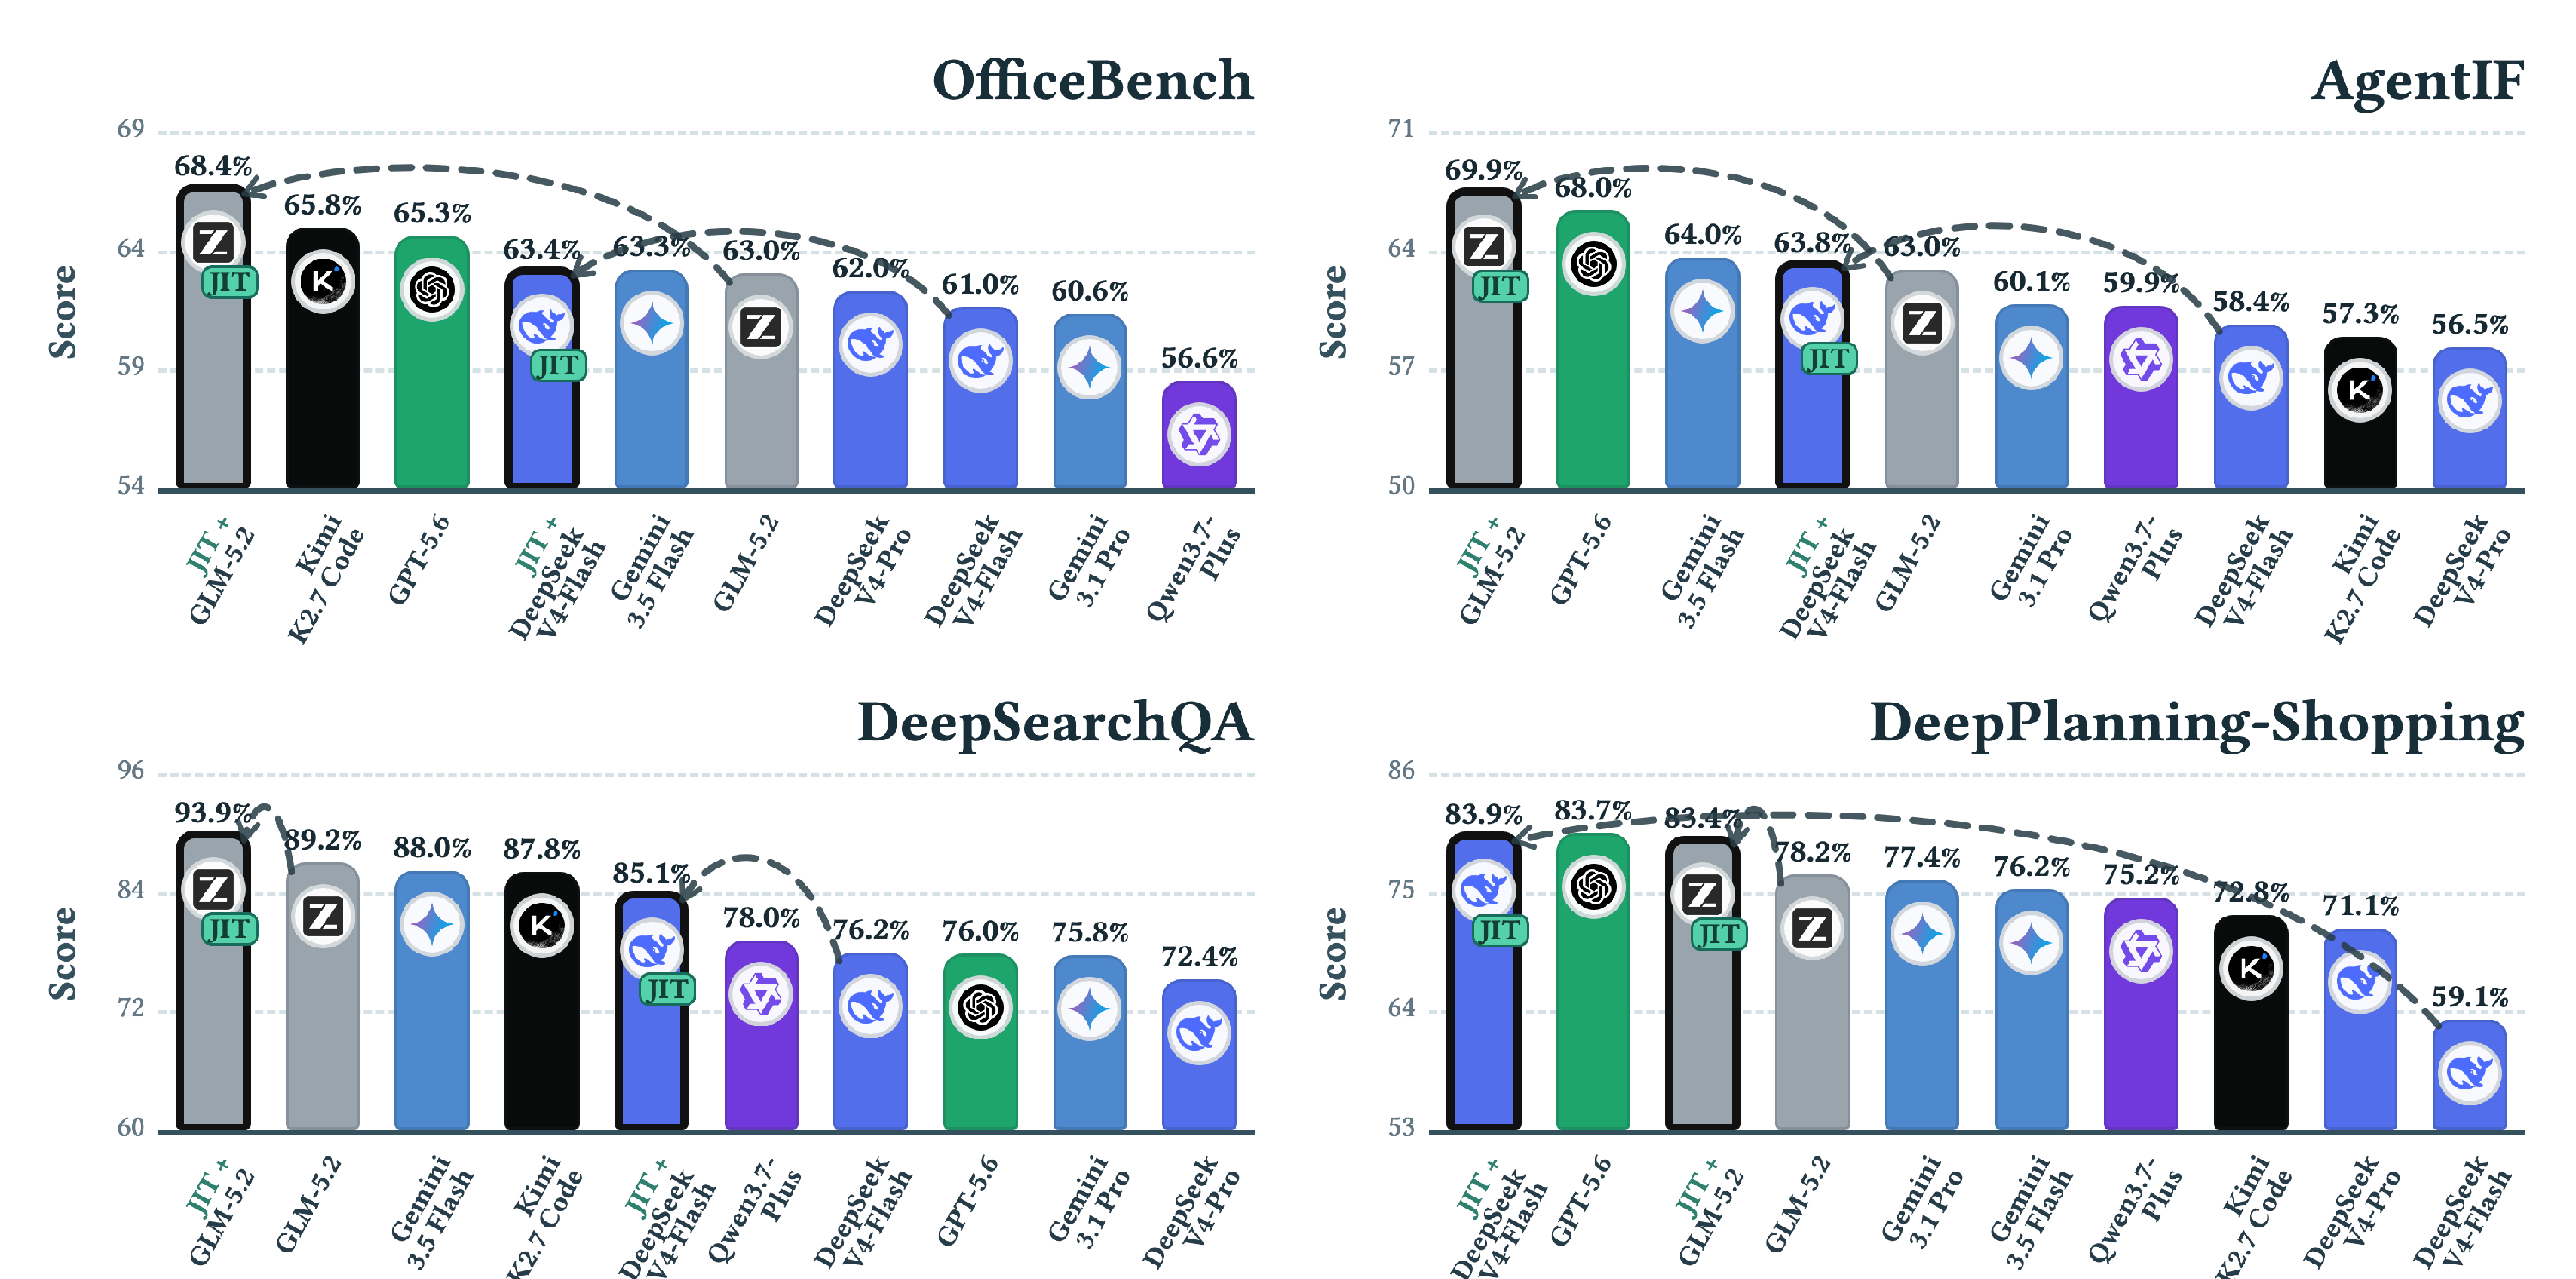
\includegraphics[width=\textwidth]{figures/four_benchmark_leaderboard.pdf}
    \vspace{-1.4em}\caption{\textbf{四个代表性智能体基准上的排行榜。}
    \ourmethod 生成的支架在深度研究、日常工作、规划和工作区任务上持续提升底层骨干智能体，表明即时支架合成带来的收益超出了单纯扩展模型的效果。}
    \label{fig:leaderboard_4benchmarks}
\end{figure}



\section{引言}

\label{sec:introduction}
{智能体支架至关重要。}
大语言模型智能体的能力由两个紧密耦合的因素共同决定：产生推理与动作的\textit{基础模型}，以及将该模型置于闭环执行环境中的\textit{智能体支架}~\citep{meng2026agent,zhou2026externalizationllmagentsunified,ning2026code}。
支架决定保留哪些历史、如何形成局部意图、暴露哪些工具或技能、如何执行动作，以及何时触发验证或恢复~\citep{meng2026agent,zhou2026externalizationllmagentsunified}。
强模型若置于错误的记忆、规划器或动作协议之后也可能失败；反过来，强支架也只有在模型能够理解并遵循它时才能释放能力~\citep{lee2026metaharnessendtoendoptimizationmodel,lin2026agenticharnessengineeringobservabilitydriven}。
因此，智能体的智能并非模型权重独有的属性，而是模型--支架组合的属性~\citep{lee2026metaharnessendtoendoptimizationmodel,zhou2026externalizationllmagentsunified}。
由此，支架设计不是实现细节，而是决定智能体性能的一阶因素~\citep{meng2026agent,lin2026agenticharnessengineeringobservabilitydriven}。

\paragraph{预先（AOT）支架。} 上述观察催生了越来越多关于测试时支架优化的研究~\citep{lee2026metaharnessendtoendoptimizationmodel,lin2026agenticharnessengineeringobservabilitydriven}。
近期系统从轨迹和反馈中优化支架代码、提示、工具、记忆、技能或控制策略，在编码、终端使用、Web 交互和通用智能体领域取得了显著改进~\citep{lee2026metaharnessendtoendoptimizationmodel,lin2026agenticharnessengineeringobservabilitydriven}。
尽管这些方法彼此不同，许多方法都共享一个\textit{预先}（Ahead-of-Time, AOT）假设：将支架视为在经验流上持续优化的耐久工件，并期望所得工件能够泛化至未来的任务、领域或模型版本~\citep{lee2026metaharnessendtoendoptimizationmodel,lin2026agenticharnessengineeringobservabilitydriven}。
当部署分布稳定且同质时，这是一个强大的范式~\citep{lin2026agenticharnessengineeringobservabilitydriven,zhang2025memevolve}。
然而，它仍要求优化环在看到每个未来问题的确切结构之前，预先编译出一个普遍有用的支架~\citep{lee2026metaharnessendtoendoptimizationmodel}。




\paragraph{即时（JIT）支架。} 我们转而采用一种\textbf{\textit{即时}（Just-in-Time, JIT）的支架构建观}。
不同任务显然需要不同的支架先验。
广域搜索任务可能受益于并行证据探索~\citep{qin2025flashsearcherfasteffectiveweb}；终端任务通常更适合精简、串行的 ReAct 环~\citep{yao2023reactsynergizingreasoningacting,merrill2026terminalbenchbenchmarkingagentshard}；深度研究任务需要围绕检索证据维护工作记忆~\citep{hu2025memoryageaiagentssurvey}；而 NL2Repo 风格的编码任务则天然由文件系统居中协调，文件系统存放补丁、测试、轨迹和仓库状态~\citep{yang2024sweagentagentcomputerinterfacesenable,ning2026code}。
简言之，合适的支架不仅取决于领域，还取决于具体实例~\citep{meng2026agent,zhou2026externalizationllmagentsunified}。
面对这些异质需求，优化单个 AOT 支架十分繁琐：系统必须搜索庞大的设计空间、积累足够多的轨迹，然后期待所得脚手架恰好适配下一项任务~\citep{lee2026metaharnessendtoendoptimizationmodel,lin2026agenticharnessengineeringobservabilitydriven}。
我们由此追问另一种可能性是否可行：\textbf{模型即支架（Model-as-a-Harness）}，即由训练过的元智能体现场生成任务专用支架，再由任意智能体大语言模型在该支架下执行。



\begin{figure}[!t]
    \centering
    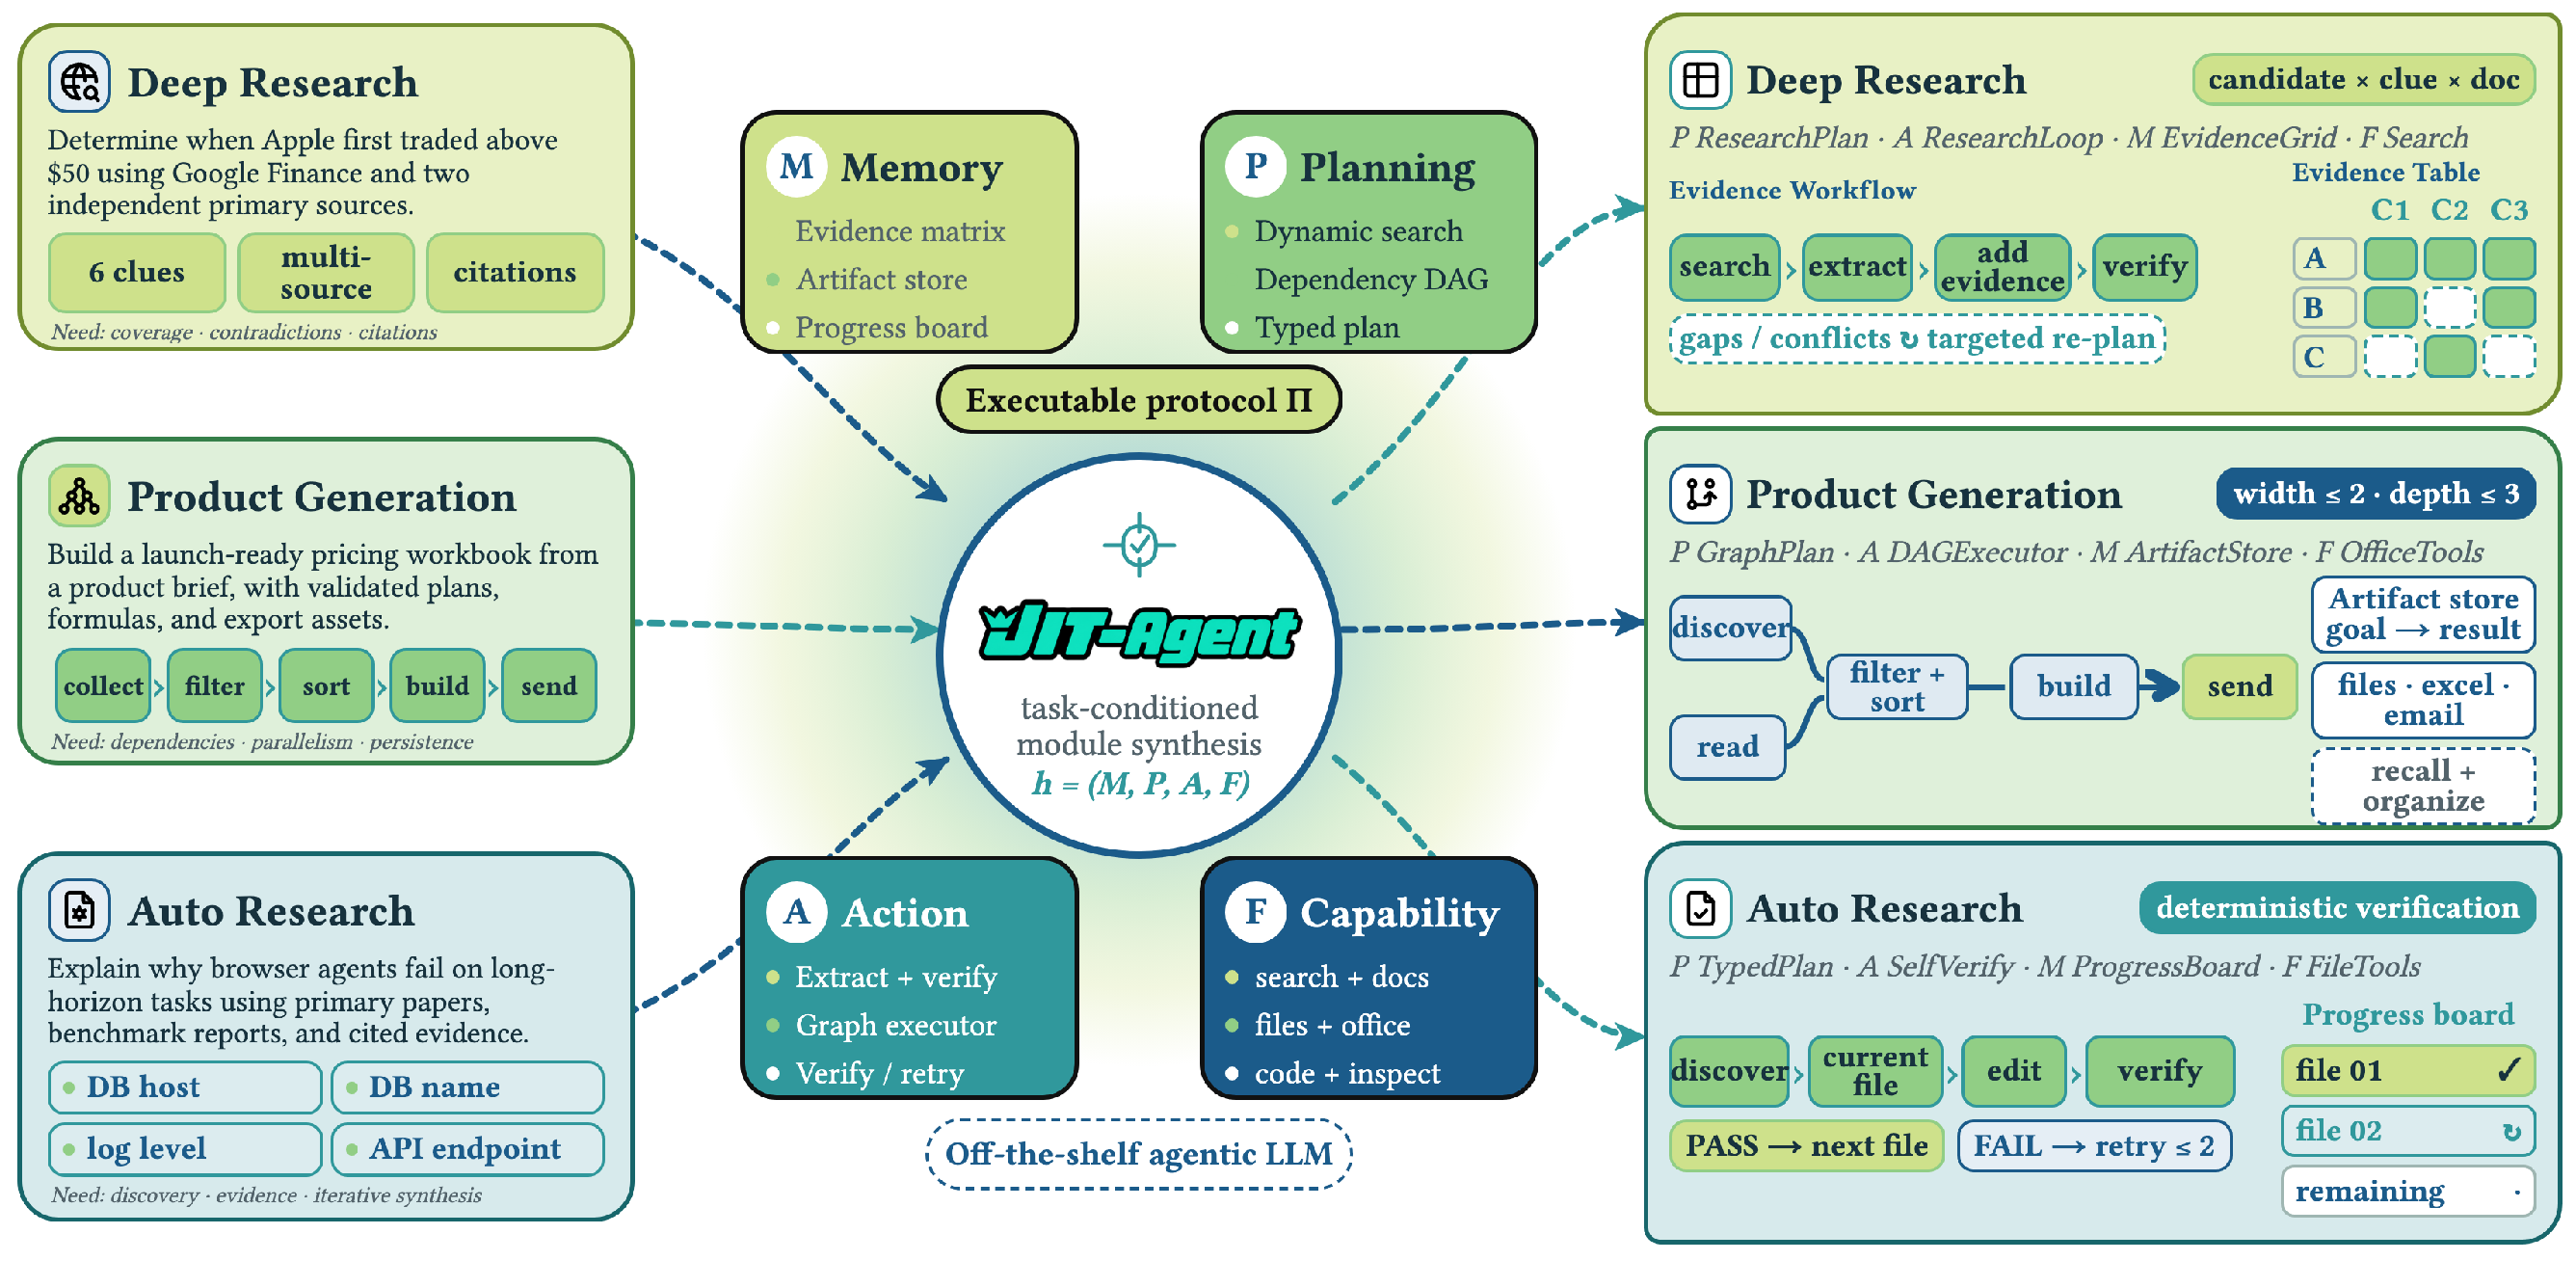
\includegraphics[width=\textwidth]{figures/jit_method_overview_final.pdf}
    \caption{\textbf{JIT-Agent 概览。}
给定一项任务，JIT-Agent 通过实例化（而非简单拼接）记忆、规划、动作和能力四个模块，构造面向该问题的智能体支架。因此，不同的任务结构会诱导出不同的可执行协议与状态组织方式；图中分别展示了面向深度研究、产品生成和自主研究的专用支架。}
    \label{fig:overview}
\end{figure}

\paragraph{JIT-Agent。} 我们提出 \ourmethod，一种用于即时支架生成与演化的紧凑元智能体。\footnote{\ourmethod 延续了我们推动智能体系统递归自设计与自演化的整体工作。在将支架作为整体处理之前，我们已研究单个支架组件层面的模块化设计与演化：\textsc{MemEvolve} 中的记忆~\citep{zhang2025memevolve} 和 \textsc{TodoEvolve} 中的规划~\citep{liu2026todoevolve}。\ourmethod 是这条研究路线的统一延伸，将组件级自设计拓展到完整的运行支架。}
在推理时，\ourmethod{} 接收任务规范、协议、可执行工具/技能注册表，以及检索得到的一小段既往支架上下文，并输出为手头任务量身定制的可执行支架。
所得支架包装一个现成的智能体大语言模型并负责执行。随着反馈与轨迹不断积累，\ourmethod{} 可修订支架并更新支架档案，从而在生成器本身保持固定的情况下实现测试时支架演化。
训练这样的系统面临三项挑战：
\ding{182} \textbf{适应性}，即如何让生成的支架匹配任务；
\ding{183} \textbf{可靠性}，即如何保证行为可执行，并在合成失败时恢复~\citep{pan2026natural,ning2026code}；以及
\ding{184} \textbf{可演化性}，即如何将执行反馈转化为未来更强的支架~\citep{lee2026metaharnessendtoendoptimizationmodel,lin2026agenticharnessengineeringobservabilitydriven}。
这三项要求共同定义了我们所说的\textbf{支架智能}：

\begin{insightbox}{支架智能}
支架智能是构建并完善模型赖以行动的运行脚手架的能力。它有三个决定性属性：\textbf{适应性}，使支架匹配任务与骨干模型；\textbf{可靠性}，产生可执行行为，并在合成失败时恢复；\textbf{可演化性}，将执行反馈转化为未来更强的支架。固定支架内的能力抵达边界之处，正是支架智能开始之处。
\end{insightbox}

\ourmethod 在协议诱导的支架空间上采用三阶段训练方案来实现支架智能~\citep{meng2026agent,zhou2026externalizationllmagentsunified}。
首先，我们将智能体支架分解为由\textit{记忆}、\textit{规划}、\textit{动作}和\textit{能力编排}模块组成的四元组，并构建 \textsc{HarnessFactory}：在这一公共接口下汇集代表性脚手架的统一代码库~\citep{hu2025memoryageaiagentssurvey,erdogan2025plan,yao2023reactsynergizingreasoningacting,xu2026agentskillslargelanguage}。
遵循“\textit{代码承载支架}”的观点~\citep{ning2026code,pan2026natural}，这一表示使支架生成成为可能：\ourmethod{} 生成结构化的可执行模块，而不是不受约束的智能体程序。
随后，\textbf{\ding{182} 阶段 I} 从教师生成的协议合规样例中学习任务条件化定制，使生成器在共享设计空间中具备适应性。
其次，\textbf{\ding{183} 阶段 II} 将失败的生成结果转化为有界修复轨迹，把编译器错误、接口不匹配和运行时故障变成可靠恢复的监督信号。
第三，\textbf{\ding{184} 阶段 III} 引入\textit{演化式组解耦策略优化}（Evolutionary Group-Decoupled Policy Optimization, Evo-GDPO），分别归一化奖励、延迟和成本，同时优化 \ourmethod{}，使其提出能够超越当前档案前沿的支架。
这一步把测试时支架改进从外部搜索启发式转变为训练所得能力，从而提供可演化性。
通过这条流水线，我们训练得到 \textbf{JIT-Agent-27B}，一种能够定制、修复和演化任务专用支架的\textbf{支架智能模型}，将支架工程从 AOT 工件转向原生 JIT 合成。

\paragraph{实验发现。}
结果表明，支架智能既能提升高效骨干模型，也能进一步拓展本已强大的模型。配备 \ourmethod 的 {DeepSeek-V4-Flash} 在 DeepSearchQA、PinchBench 和 OdysseyBench 上分别超过 GPT-5.6 $9.1$、$8.7$ 和 $4.3$ 分。对于本已强大的 {GLM-5.2}，\ourmethod 进一步抬高上限，在 xBench-DS 和 AgentIF 上分别取得 $+12.0$ 和 $+6.9$ 的显著绝对增益。除这些醒目的结果外，\ourmethod 生成的支架在性能上可与 OpenCode、Claude Code 等成熟智能体运行时竞争，并能在 DeepSeek V4、Mimo-V2.5 和 Qwen3.6 不同规模的变体上持续带来收益。

\paragraph{贡献。} 我们的贡献概括如下：
\vspace{-0.4em}
\begin{itemize}[itemsep=-0.1em]
    \item[\ding{227}] \textbf{支架智能。}
    我们将\textit{模型即支架}形式化为一种新的智能体改进范式，并把\textit{支架智能}定义为通过学习获得的、构建、修复和演化智能体运行脚手架的能力。

    \item[\ding{227}] \textbf{实用方案。}
    我们提出 \ourmethod{} 及其三阶段训练流水线，结合四模块可执行支架协议、\textsc{HarnessFactory}、定制学习、反馈驱动修复，以及用于测试时支架演化的 Evo-GDPO。

    \item[\ding{227}] \textbf{实验验证。}
    我们在异质智能体基准和模型骨干上验证 \ourmethod{}，结果表明 JIT 生成的支架能够改善原生智能体、与强大的固定支架竞争，并推动骨干--支架组合迈向更优的成本--性能前沿。
\end{itemize}




\section{相关工作}


\paragraph{支架工程与模块化。} 支架工程仍呈现出显著的多样性，覆盖 Claude Code、Codex、Hermes 和 OpenClaw 等编码与通用运行时~\citep{githubGitHubAnthropicsclaudecode,openaiCodexCoding,nous2026hermes,openclaw2026}、具身系统~\citep{zhang2026harnessvla,lee2026physicalaiharness}、搜索智能体~\citep{apodex2026,qin2025flashsearcherfasteffectiveweb}，以及 Mem0、EverMemOS 和 MemEvolve 等以记忆为中心的支架~\citep{chhikara2025mem0,hu2026evermemos,zhang2025memevolve}。在这些差异之下，支架是决定智能体观察、记忆、规划、调用、验证和执行内容的运行层，因此能力是模型--支架组合而非模型权重本身的属性~\citep{meng2026agent,zhou2026externalizationllmagentsunified,pan2026natural,lee2026metaharnessendtoendoptimizationmodel}。反复出现的设计选择包括：\textbf{(i) 记忆}，用于整理工作上下文并保存跨会话经验~\citep{hu2026memoryageaiagents,hu2024hiagenthierarchicalworkingmemory,yan2025generalagenticmemorydeep,zhang2025memoryactionautonomouscontext}；\textbf{(ii) 规划}，形成并修订子目标，以更新智能体的行动方向~\citep{cao2025largelanguagemodelsplanning,erdogan2025planandactimprovingplanningagents,jin2025hirahierarchicalreasoningframework,qin2025flashsearcherfasteffectiveweb}；\textbf{(iii) 控制环与目标管理}，执行目标、监控进度、反思结果并从失败中恢复~\citep{yao2023reactsynergizingreasoningacting,reflexion,madaan2023selfrefine,sun2023adaplanner}；\textbf{(iv) 工具分配}，从大型 API 空间中选择可调用资源并确定其顺序~\citep{qin2023toolllm,yang2026efficientagentsmemorytool,qian2025toolrl,wang2025otc}；以及\textbf{(v) 技能编排}，从不断增长的技能库中发现、检索、组合和委派可复用过程~\citep{xu2026agentskillslargelanguage,zheng2025skillweaver,li2026agentskillos,zhou2026externalizationllmagentsunified}。因此，模块化已成为该领域共同的设计语言：表示方式可以不同，但显式接口使支架组件能够独立替换与优化~\citep{chen2026harnessx,ning2026code,pan2026natural,lin2026agenticharnessengineeringobservabilitydriven,lee2026metaharnessendtoendoptimizationmodel}。例如，HarnessX 将运行时分解为提示、工具、记忆和控制流，而 Code-as-Agent-Harness 则将其组织为接口、机制和多智能体扩展层~\citep{chen2026harnessx,ning2026code}。因此，我们采用紧凑分解 $\mathbf{h}=(\mathbf{M},\mathbf{P},\mathbf{A},\mathbf{F})$，四个模块分别构建记忆视图、形成下一条指令、推进动作环并编排工具与技能；它提供最小可执行契约，同时保留每个模块内部的可扩展性~\citep{hu2026memoryageaiagents,cao2025largelanguagemodelsplanning,yao2023reactsynergizingreasoningacting,xu2026agentskillslargelanguage}。

\paragraph{支架优化。} 完成模块化后，支架构建便从固定的工程选择转变为针对可执行工件的优化问题~\citep{khattab2023dspy,yuksekgonul2024textgradautomaticdifferentiationtext,hu2024adas,shang2024agentsquare}。优化范围已从提示与声明式语言模型流水线扩展至工作流图、角色分配和完整支架代码，使反馈既能修改局部指令，也能修改全局控制结构~\citep{khattab2023dspy,zhang_aflow_2024,hu2024adas,shang2024agentsquare,lee2026metaharnessendtoendoptimizationmodel}。\textbf{闭环演化。} 在支架层面，近期方法大多实现“诊断--提议--验证”循环：执行轨迹暴露行为弱点，候选编辑修改提示、记忆、工具、中间件或控制流，而验证或偏好信号决定哪些更改得以保留~\citep{lee2026metaharnessendtoendoptimizationmodel,lin2026agenticharnessengineeringobservabilitydriven,zhang2026selfharness,pan2026retrospectiveharness,chen2026harnessx}。近期工作进一步将这一循环扩展到递归式、层次式和协作式自我改进，同时约束逐组件演化以改善迁移~\citep{lee2026recursiveharness,zhou2026hierarchicalselfimprovement,nie2026evolvenet,zhang2026harnesscompass}。其监督形式从文本梯度和以轨迹为依据的可观测性，到回归测试、回溯式自偏好和有类型原语替换不等，但共同产物都是持续改进的可执行脚手架~\citep{yuksekgonul2024textgradautomaticdifferentiationtext,lin2026agenticharnessengineeringobservabilitydriven,zhang2026selfharness,pan2026retrospectiveharness,chen2026harnessx}。\textbf{AOT 与 JIT。} 尽管这些支架可能具备迁移性，这些方法主要仍依据累积的经验分布优化一个耐久工件；相对于新实例的确切结构而言，它们属于预先方法~\citep{zhang_aflow_2024,zhang2025maas,yuan2024evoagent,chen2023evoprompting}。我们则将支架搜索摊销到 \ourmethod 中：生成器在推理时合成任务条件化支架，并可依据执行反馈进一步修订它，使优化从重复的工件搜索转向学习得到的即时构建~\citep{meng2026agent,zhou2026externalizationllmagentsunified,ning2026code,pan2026natural,xu2026agentskillslargelanguage}。\Cref{tab:harness_optimization_comparison} 明确展示了这一区别。

\begin{table}[!t]
\centering
\caption{\small \textbf{支架优化范式。}\emph{构建方式}区分预先搜索得到的支架、随后由测试时反馈编辑的预先支架，以及为每项任务即时生成的支架。\emph{实例合成}、\emph{支架模型}、\emph{学习式修复}和\emph{在线演化}分别表示一种方法是否直接合成实例专用支架、训练生成器、从失败执行轨迹中学习修复，以及在部署后持续改进。}
\label{tab:harness_optimization_comparison}
\footnotesize
\setlength{\tabcolsep}{3pt}
\renewcommand{\arraystretch}{0.9}
\begin{tabular}{@{}>{\RaggedRight\arraybackslash}p{0.30\textwidth} >{\centering\arraybackslash}p{0.20\textwidth} *{4}{c}@{}}
\toprule
方法 & 构建方式 & \shortstack{实例\\合成} & \shortstack{支架\\模型} & \shortstack{学习式\\修复} & \shortstack{在线\\演化} \\
\midrule
AutoHarness~\citep{lou2026autoharness} & AOT（搜索） & \xmark & \xmark & \xmark & \xmark \\
Meta-Harness~\citep{lee2026metaharnessendtoendoptimizationmodel} & AOT（搜索） & \xmark & \xmark & \xmark & \xmark \\
AHE~\citep{lin2026agenticharnessengineeringobservabilitydriven} & AOT（搜索） & \xmark & \xmark & \xmark & \xmark \\
Adaptive AH~\citep{liu2026adaptiveautoharness} & AOT（测试时编辑） & \xmark & \xmark & \xmark & \cmark \\
TTHE~\citep{nie2026tthe} & AOT（测试时编辑） & \xmark & \xmark & \xmark & \cmark \\
RHI~\citep{lee2026recursiveharness} & AOT（测试时编辑） & \xmark & \xmark & \xmark & \cmark \\
Harness-R1~\citep{shao2026harnessr1} & AOT（测试时编辑） & \xmark & \cmark & \cmark & \cmark \\
\midrule
\textbf{\ourmethod（本文）} & \textbf{JIT} & \cmark & \cmark & \cmark & \cmark \\
\bottomrule
\end{tabular}
\end{table}




\section{统一支架代码库}
\label{sec:harness_codebase}

\subsection{模块化支架设计空间}
智能体支架是将基础模型转化为闭环智能体的运行层~\citep{202604.0428,zhou2026externalizationllmagentsunified}：它决定保留既往交互中的哪些内容~\citep{hu2026memoryageaiagents}、如何形成中间指令~\citep{cao2025largelanguagemodelsplanning}、每个阶段暴露哪些外部能力~\citep{xu2026agentskillslargelanguage,yang2026efficientagentsmemorytool}，以及如何推进控制。因此，支架生成定义在程序而非不受约束的文本之上。我们区分原始生成空间 $\mathcal{G}$、语法有效的支架 $\mathcal{H}^{\mathrm{syn}}$、符合协议的支架 $\mathcal{H}_{\boldsymbol{\Pi}}$ 及其中的可执行子集 $\mathcal{H}^{\mathrm{exec}}_{\boldsymbol{\Pi}}$，它们满足 $\mathcal{G}\supseteq\mathcal{H}^{\mathrm{syn}}\supseteq\mathcal{H}_{\boldsymbol{\Pi}}\supseteq\mathcal{H}^{\mathrm{exec}}_{\boldsymbol{\Pi}}$。固定协议 $\boldsymbol{\Pi}$ 规定模块模式与接口、模块生命周期、验证规则和共享执行语义。它消除了语言和运行时中的偶然差异，同时保留区分现有支架的主要运行选择~\citep{autogen,githubGitHubAg2aiag2,githubGitHubLangchainailanggraph,luo2025largelanguagemodelagent}。

\begin{insightbox}{支架可组合性}
可组合性已成为现代支架设计中的一等关切。例如，DeepSeek Harness 采用“万物皆插件”（Everything is a Plugin）的架构，将运行时表示为通过显式依赖关系连接的模块~\citep{shi2026spatiotemporalcomposability}。可组合性对于 JIT 生成同样关键：它把支架构建从不受约束的程序合成转化为在有类型、可重组设计空间中的装配。
\end{insightbox}

\ourmethod 通过四个可互操作模块显式表达这些选择：\textit{如何压缩历史}、\textit{如何形成局部意图}、\textit{如何编排工具与技能}，以及\textit{如何推进控制}。令 $\boldsymbol{\tau}$ 为一项任务，$\pi_{\psi}$ 为冻结的骨干执行器，$\mathcal{C}_{\tau}$ 为该任务可用的能力注册表（\textit{例如}工具、API 和技能）。使用 $\pi_{\psi}$ 运行支架 $\mathbf{h}$ 会产生闭环轨迹
\begin{equation}
\label{eq:trajectory}
    \boldsymbol{\xi}
    \sim \operatorname{Rollout}(\boldsymbol{\tau},\pi_{\psi},\mathbf{h},\mathcal{C}_{\tau};\boldsymbol{\Pi})
    = \bigl(\mathbf{s}_1,e_1,\mathbf{o}_1,\ldots,\mathbf{s}_T,e_T,\mathbf{o}_T\bigr),
\end{equation}
其中，$\mathbf{s}_t\in\mathcal{S}$ 是所维护的控制器状态，$e_t$ 是发出的工具调用或终止输出，$\mathbf{o}_t\in\mathcal{O}$ 是所得观察，而 $T$ 是由协议或预算限制的停止时刻。我们的关键假设是，每个 $\mathbf{h}\in\mathcal{H}_{\boldsymbol{\Pi}}$ 都允许如下模块化分解：
\begin{equation}
\label{eq:harness_decomp}
    \mathbf{h} \,=\, \bigl(\mathbf{M},\, \mathbf{P},\, \mathbf{A},\, \mathbf{F}\bigr)
    \in
    \mathfrak{M} \times \mathfrak{P} \times \mathfrak{A} \times \mathfrak{F},
\end{equation}
其中，$\mathbf{M}$、$\mathbf{P}$、$\mathbf{A}$ 和 $\mathbf{F}$ 分别表示记忆、规划、动作和能力编排模块，而 $\mathfrak{M}$、$\mathfrak{P}$、$\mathfrak{A}$ 和 $\mathfrak{F}$ 是各自与协议兼容的实现空间。该元组遵循上述概念分解；在运行时，其依赖顺序为 $\mathbf{M}\!\rightarrow\!\mathbf{P}\!\rightarrow\!\mathbf{F}\!\rightarrow\!\mathbf{A}$。所有模块都面向同一个冻结的 $\pi_{\psi}$ 运行，下文省略这种共同的运行时依赖。



\begin{insightbox}{定位}
Codex、Claude Code 和 DeepSeek Harness 等生产级支架所暴露的机制远比我们的四模块实例丰富~\citep{shi2026spatiotemporalcomposability,githubGitHubAnthropicsclaudecode,openaiCodexCoding}。这一差距是有意为之。本工作并非要求模型复现完整的生产运行时，而是要确立一个更基础的结果：即便支架十分紧凑，只要即时生成，也能带来显著收益。此外，我们认为 JIT 范式与生产支架工程互为补充。随着模型越来越多地参与自身运行时的设计与修订，支架智能的训练方案在更大规模上也会同样重要。我们将当前设计空间视为一个起点。
\end{insightbox}

该协议同时维护不可变事件历史 $\boldsymbol{\xi}_{<t}$ 和可变控制器状态 $\mathbf{s}_t$，二者按如下方式交互：
\begin{align}
    \mathbf{v}_t &= \mathbf{M}(\boldsymbol{\xi}_{<t},\mathbf{s}_t) \in \mathcal{V},
    && \text{历史 $\to$ 视图，} \label{eq:memory} \\
    \mathbf{d}_t &= \mathbf{P}(\boldsymbol{\tau},\mathbf{s}_t,\mathbf{v}_t) \in \mathcal{D}_{\mathrm{dir}},
    && \text{视图 $\to$ 局部指令，} \label{eq:planning} \\
    \mathcal{C}_t &= \mathbf{F}(\mathcal{C}_{\tau},\mathbf{s}_t,\mathbf{v}_t,\mathbf{d}_t) \subseteq \mathcal{C}_{\tau},
    && \text{以指令为条件的能力编排，} \label{eq:toolpolicy} \\
    (\mathbf{s}_{t+1},e_t) &= \mathbf{A}(\mathbf{s}_t,\boldsymbol{\tau},\mathbf{v}_t,\mathbf{d}_t,\mathcal{C}_t) \in \mathcal{S}\times\mathcal{A},
    && \text{控制更新与动作发出，} \label{eq:action}
\end{align}
其中，$\mathcal{V}$ 和 $\mathcal{D}_{\mathrm{dir}}$ 分别是视图空间和指令空间，$\mathcal{A}=\mathcal{U}\sqcup\mathcal{Y}$ 是可执行调用与终止输出的不交并。注册表 $\mathcal{C}_{\tau}$ 包含可调用工具（\textit{例如} bash 工具、API 和 MCP~\citep{sarkar2025surveyllmagentcommunication}）以及更高层的智能体技能~\citep{xu2026agentskillslargelanguage,claudeAgentSkills}。没有显式规划器的支架仍可通过空指令 $\mathbf{d}_{\emptyset}\in\mathcal{D}_{\mathrm{dir}}$ 保持类型一致；$\mathbf{P}_{\emptyset}$ 会在每一步返回该空指令。
换言之，记忆从已实现历史中构建视图，规划将该视图转化为局部指令，能力编排激活相关外部工具或智能体技能，而动作模块使用组装后的上下文，同时更新控制器状态并发出下一动作。内核随后按如下方式解释发出的动作：
\begin{equation}
\label{eq:kernel}
    \mathbf{o}_t
    \,=\,
    \begin{cases}
        \operatorname{Exec}(e_t;\mathcal{C}_t), & e_t \in \mathcal{U}, \\
        \bot, & e_t \in \mathcal{Y},
    \end{cases}
    \qquad
    \boldsymbol{\xi}_{\le t} \,=\, \boldsymbol{\xi}_{<t} \oplus (\mathbf{s}_t,e_t,\mathbf{o}_t),
\end{equation}
其中，$\operatorname{Exec}:\mathcal{U}\times2^{\mathcal{C}_{\tau}}\rightarrow\mathcal{O}$ 是共享执行内核，$\bot\in\mathcal{O}$ 是终止空观察，$\oplus$ 表示向轨迹追加一个事件。执行从 $\boldsymbol{\xi}_{<1}=\emptyset$ 和协议定义的 $\mathbf{s}_1\in\mathcal{S}$ 开始，在 $e_t\in\mathcal{Y}$ 时终止，并产生 $y=e_T\in\mathcal{Y}$。这一分解把原本异质的程序转化为 $\mathfrak{M}\times\mathfrak{P}\times\mathfrak{A}\times\mathfrak{F}$ 中可比较的坐标：
\begin{itemize}[itemsep=0.15em, topsep=0.3em]
    \item \textbf{标准 ReAct} 可写作 $\mathbf{h}_{\mathrm{ReAct}} = (\mathbf{M}_{\mathrm{full}}, \, \mathbf{P}_{\emptyset}, \, \mathbf{A}_{\mathrm{react}}, \, \mathbf{F}_{\mathrm{all}})$，其中 $\mathbf{A}_{\mathrm{react}}$ 是标准 ReAct 环，$\mathbf{P}_{\emptyset}$ 表示没有显式规划器，$\mathbf{M}_{\mathrm{full}}$ 不做上下文管理而保留运行历史，$\mathbf{F}_{\mathrm{all}}$ 则暴露完整的工具/技能注册表。
    \item Codex~\citep{openaiCodexCoding} 和 OpenCode~\citep{githubGitHubOpencodeaiopencode} 等\textbf{工程化 ReAct 变体}仍符合相同的脚手架：$(\mathbf{M}_{\mathrm{compact}}, \, \mathbf{P}_{\mathrm{todo}}, \, \mathbf{A}_{\mathrm{react}}, \, \mathbf{F}_{\mathrm{all}})$。其中动作内核仍为 ReAct 风格，但 $\mathbf{M}_{\mathrm{compact}}$ 会在接近上下文上限时压缩历史，而 $\mathbf{P}_{\mathrm{todo}}$ 维护显式的任务待办列表。
    \item \textbf{递归智能体。} ROMA~\citep{alzubi2026romarecursiveopenmetaagent}、AOrchestra~\citep{ruan2026aorchestraautomatingsubagentcreation} 和递归语言模型（RLM）~\citep{zhang2026recursivelanguagemodels} 等递归架构同样可以由 $\mathbf{h}_{\mathrm{rec}} = (\mathbf{M}_{\mathrm{subproblem}}, \, \mathbf{P}_{\mathrm{decomp}}, \, \mathbf{A}_{\mathrm{rec}}, \, \mathbf{F}_{\mathrm{route}})$ 之类的选择刻画。在此类系统中，主编排器可通过 $\mathbf{A}_{\mathrm{rec}}$ 生成子智能体，在 $\mathbf{P}_{\mathrm{decomp}}$ 中维护待办式分解，在 $\mathbf{M}_{\mathrm{subproblem}}$ 中隔离智能体上下文，并通过 $\mathbf{F}_{\mathrm{route}}$ 向每个子智能体分配工具或技能。
\end{itemize}


\begin{table}[!t]
\setcitestyle{numbers,square}
\centering
\caption{种子库 $\mathcal{B}_0$：13 个手工编写的支架，均实例化四模块协议 $\boldsymbol{\Pi}$。每一行都是一个完整支架；各列依次对应记忆、规划、动作和能力编排。}
\label{tab:seed_harnesses}
\setlength{\tabcolsep}{5pt}
\renewcommand{\arraystretch}{0.9}
\resizebox{\textwidth}{!}{\begin{tabular}{lllll}
\toprule
\rowcolor{headerbg}
    & \textcolor{tealblue}{\ding{168}}~\textbf{记忆}
    & \textcolor{tealblue}{\ding{169}}~\textbf{规划}
    & \textcolor{tealblue}{\ding{170}}~\textbf{动作}
    & \textcolor{tealblue}{\ding{171}}~\textbf{能力编排} \\
\rowcolor{headerbg} \multirow{-2}{*}{\textbf{支架}}
    & \scriptsize $\mathbf{M}\in\mathfrak{M}$
    & \scriptsize $\mathbf{P}\in\mathfrak{P}$
    & \scriptsize $\mathbf{A}\in\mathfrak{A}$
    & \scriptsize $\mathbf{F}\in\mathfrak{F}$ \\
\midrule
\textsc{ReAct}~\citep{yao2023react}
    & 完整历史
    & 无显式规划器
    & ReAct
    & 完整注册表
\\
\textsc{Plan-and-Execute}~\citep{erdogan2025planandactimprovingplanningagents}
    & 完整历史
    & 线性路线图
    & ReAct
    & 完整注册表
\\
\textsc{ReSum}~\citep{wu2026resumunlockinglonghorizonsearch}
    & ReSum 记忆
    & 无显式规划器
    & ReAct
    & 完整注册表
\\
\textsc{Flash-Searcher}~\citep{qin2025flashsearcherfasteffectiveweb}
    & 完整历史
    & DAG 规划
    & ReAct
    & 完整注册表
\\
\textsc{GAM}~\citep{yan2025generalagenticmemorydeep}
    & GAM 检索
    & DAG
    & ReAct
    & 完整注册表
\\
\textsc{MemoBrain}~\citep{qian2026memobrain}
    & 推理图
    & 无显式规划器
    & 标记引导执行
    & 完整注册表
\\
\textsc{AggAgent}~\citep{lee2026agenticaggregation}
    & 隔离的回滚历史
    & 无显式规划器
    & 多回滚聚合
    & 完整注册表
\\
\textsc{OAgent}~\citep{zhu2025oagentsempiricalstudybuilding}
    & 协调器历史
    & 无显式规划器
    & 集成投票
    & 完整注册表
\\
\textsc{AgentFold}~\citep{ye2025agentfoldlonghorizonwebagents}
    & AgentFold 记忆
    & DAG
    & ReActFold
    & 完整注册表
\\
\textsc{HiAgent}~\citep{hu2024hiagenthierarchicalworkingmemory}
    & 层次记忆
    & 无显式规划器
    & ReAct
    & 完整注册表
\\
\textsc{DeepAgent}~\citep{li2026deepagentgeneralreasoningagent}
    & 三层记忆
    & 无显式规划器
    & 标记引导执行
    & 工具搜索
\\
\textsc{ROMA}~\citep{alzubi2026romarecursiveopenmetaagent}
    & 上下文隔离
    & 原子化器 + DAG
    & 递归执行
    & 完整注册表
\\
\textsc{AOrchestra}~\citep{ruan2026aorchestraautomatingsubagentcreation}
    & 上下文隔离
    & 原子化器 + DAG
    & 递归执行
    & 智能体委派
\\
\bottomrule
\end{tabular}}
\end{table}



在这一模块化设计空间的基础上，接下来我们介绍 \textsc{HarnessFactory}。它用于检验 $\mathcal{H}_{\boldsymbol{\Pi}}$ 的表达能力，并为 \ourmethod 的元支架设计提供多样化素材。



\subsection{HarnessFactory}
在共享协议 $\boldsymbol{\Pi}$ 和公共内核下，\textsc{HarnessFactory} 重新实现了 13 个有代表性的当代智能体脚手架：\textsc{ReAct}~\citep{yao2023react}、\textsc{Plan-and-Execute}~\citep{erdogan2025planandactimprovingplanningagents}、\textsc{ReSum}~\citep{wu2026resumunlockinglonghorizonsearch}、\textsc{Flash-Searcher}~\citep{qin2025flashsearcherfasteffectiveweb}、\textsc{General Agentic Memory (GAM)}~\citep{yan2025generalagenticmemorydeep}、\textsc{MemoBrain}~\citep{qian2026memobrain}、\textsc{AggAgent}~\citep{lee2026agenticaggregation}、\textsc{OAgent}~\citep{zhu2025oagentsempiricalstudybuilding}、\textsc{AgentFold}~\citep{ye2025agentfoldlonghorizonwebagents}、\textsc{HiAgent}~\citep{hu2024hiagenthierarchicalworkingmemory}、\textsc{DeepAgent}~\citep{li2026deepagentgeneralreasoningagent}、\textsc{ROMA}~\citep{alzubi2026romarecursiveopenmetaagent} 和 \textsc{AOrchestra}~\citep{ruan2026aorchestraautomatingsubagentcreation}。它们提供异质的记忆、规划、动作与能力编排策略。因此，种子库 $\mathcal{B}_0$ 包含 $K_0=13$ 个与协议兼容的支架。
\Cref{tab:seed_harnesses} 给出了完整清单。

该库具有双重作用：从 $\mathcal{B}_0$ 采样的支架为阶段 I 合成提供锚点，而后续档案状态则提供用于评估新设计的先验种群。随着系统运行，$\mathcal{B}_0$ 增长为 $\mathcal{B}_n\supseteq\mathcal{B}_0$；其中每个条目都把保留的支架与其任务及观测到的奖励、延迟和成本关联起来。第~\ref{sec:harness_evolution}~节对这一演化过程给出形式化描述。



\begin{figure}[!t]
    \centering
    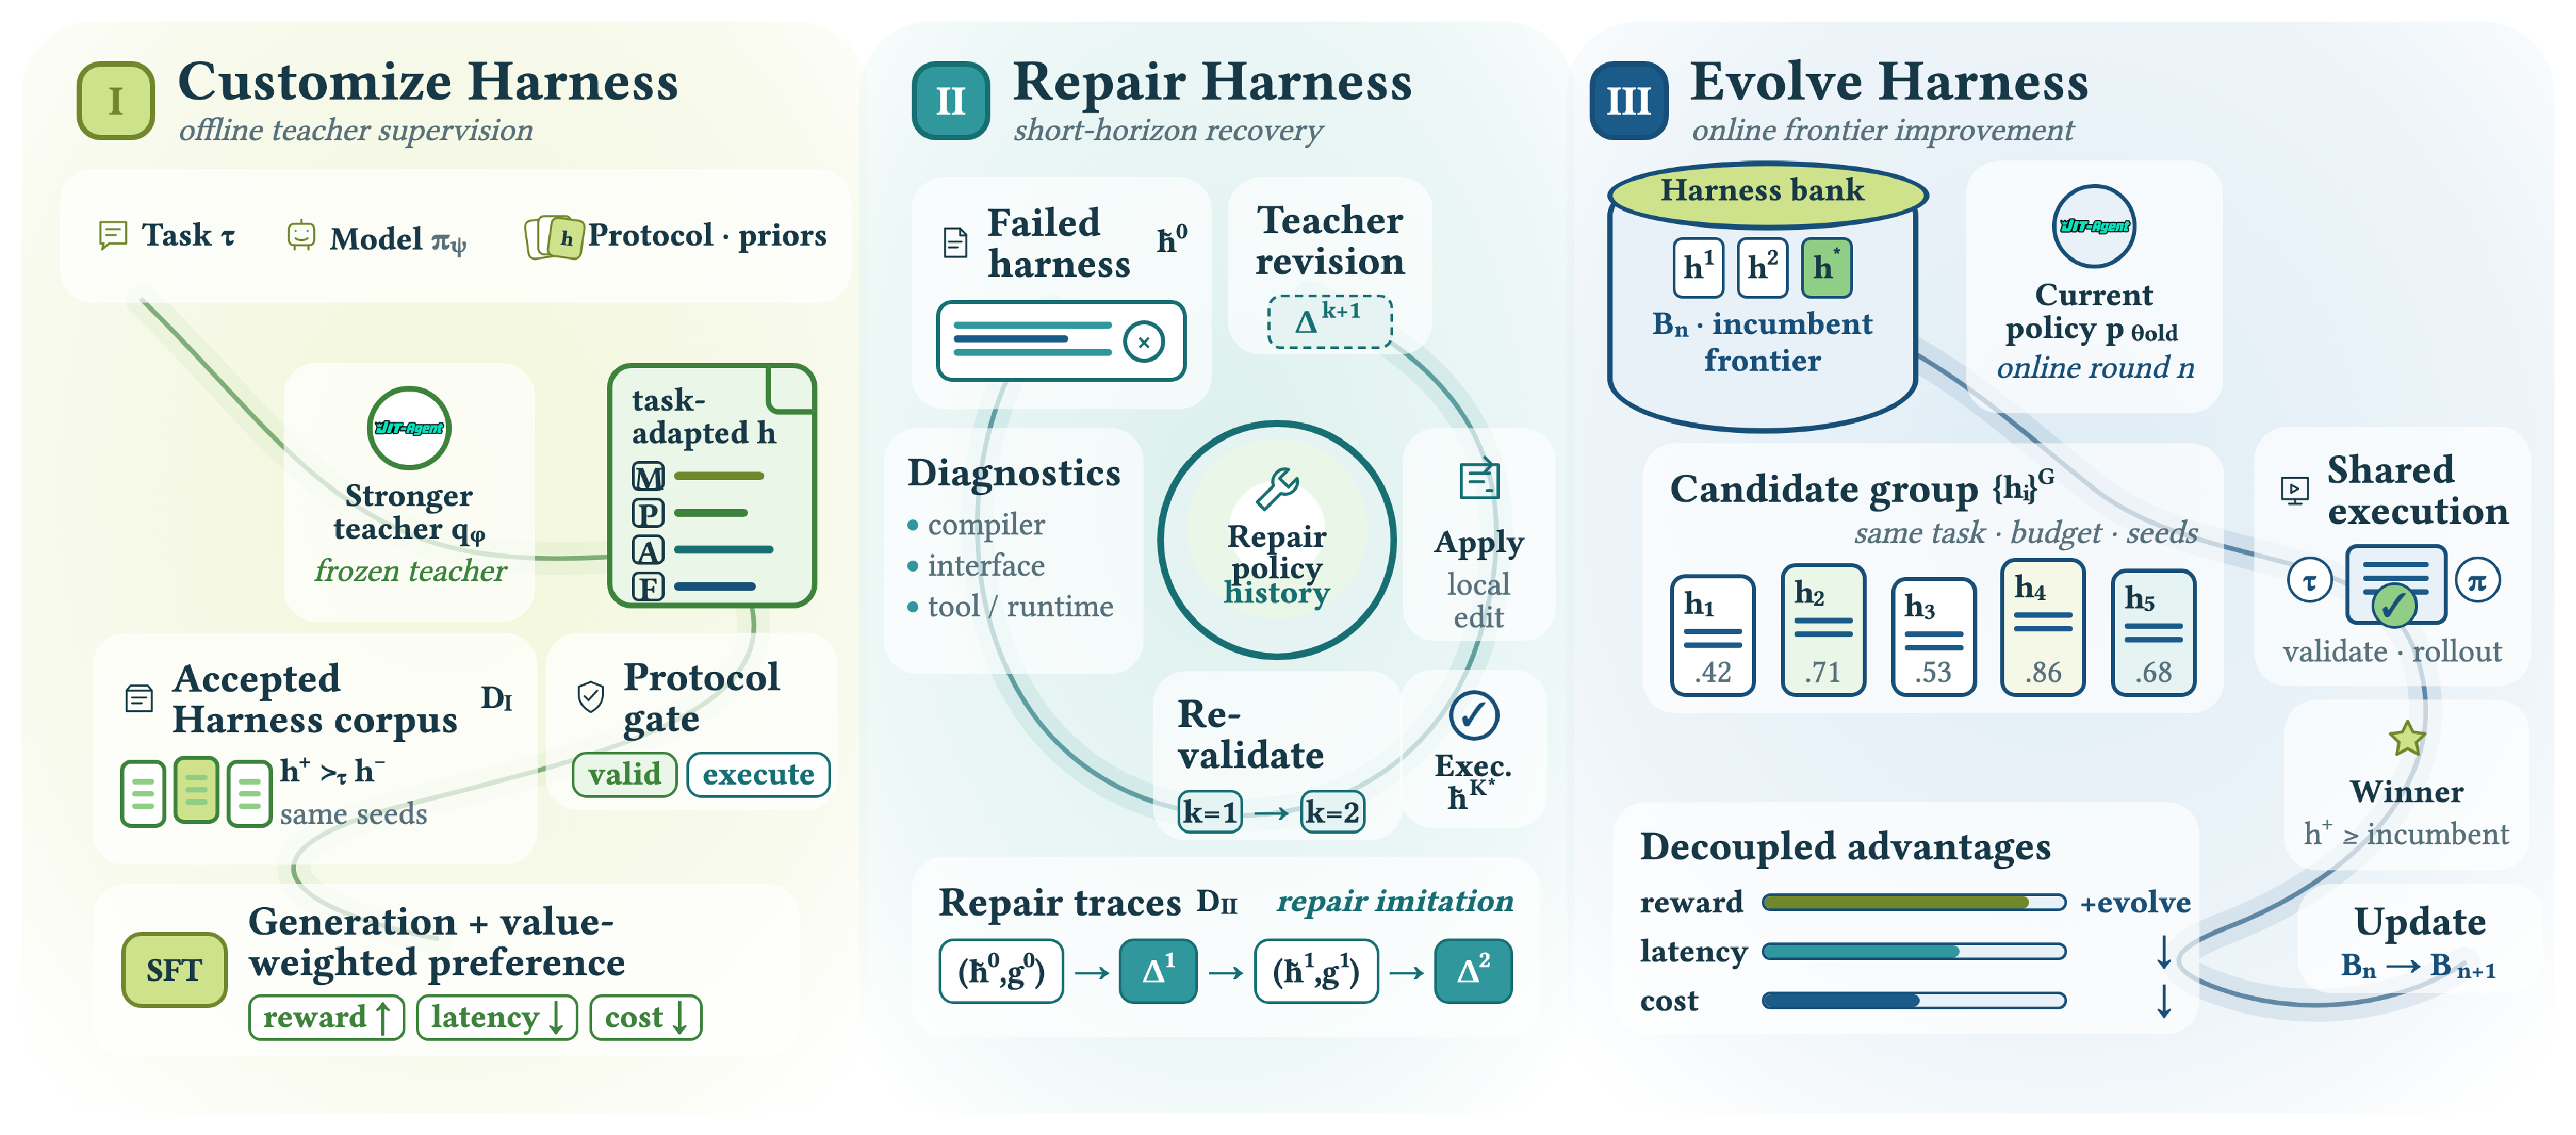
\includegraphics[width=\linewidth]{figures/jit_training_pipeline_frontier.pdf}
    \caption{\textbf{\ourmethod 的训练流水线。}阶段 I 学习任务条件化的支架定制。阶段 II 将失败支架和执行诊断转化为有界修复轨迹。阶段 III 将候选支架与当前库进行比较，优化解耦的奖励、延迟和成本优势，并保留改善前沿的设计，从而执行在线演化。}
    \label{fig:training}
\end{figure}



\section{训练流水线}\label{sec:training}

训练遵循 \ourmethod 在推理时的生命周期：首先合成任务条件化支架，然后恢复不稳定的生成结果，最后学习如何在线利用更强的档案状态继续改进。令 $\boldsymbol{\tau}\sim\mathcal{D}_{\mathrm{task}}$ 表示从训练分布中抽取的任务，$\mathcal{C}_{\tau}$ 表示其能力注册表，$\mathcal{E}_{\tau}$ 表示来自支架库的一小段参考上下文。我们将生成上下文定义为 $\mathbf{c}_{\tau}=(\boldsymbol{\tau},\boldsymbol{\Pi},\mathcal{C}_{\tau},\mathcal{E}_{\tau})$，并从 $p_{\theta}(\mathbf{h}\mid\mathbf{c}_{\tau})$ 采样支架。随后，冻结的执行器 $\pi_{\psi}\sim\mathcal{M}$ 运行每个支架，以完成验证和效用度量。共同目标为
\begin{equation}
\label{eq:training_goal}
\theta^{\star}
= \arg\max_{\theta}
\mathbb{E}_{\substack{\boldsymbol{\tau}\sim\mathcal{D}_{\mathrm{task}},\,\pi_{\psi}\sim\mathcal{M},\\
\mathbf{h}\sim p_{\theta}(\cdot\mid\mathbf{c}_{\tau})}}
\bigl[U(\boldsymbol{\tau},\pi_{\psi},\mathbf{h})\bigr],
\end{equation}
其中，$U$ 使用任务奖励、延迟和货币成本评估模型--支架组合所诱导的轨迹。由于 $p_{\theta}$ 在 $\mathcal{G}$ 中生成，并不通过构造天然满足可执行性，因此每个输出都要接受协议验证器检查。我们用 $\operatorname{Valid}_{\boldsymbol{\Pi}}(\mathbf{h};\boldsymbol{\tau},\pi_{\psi},\mathcal{C}_{\tau})\in\{0,1\}$ 表示其有效性标志；检查失败时还会返回结构化诊断报告。阶段 I 的离线监督、阶段 II 的修复轨迹学习和阶段 III 的在线策略改进共同实例化了\Cref{eq:training_goal}。

\subsection{阶段 I：定制支架}\label{sec:scaffold_synthesis}

\paragraph{数据准备。}
阶段 I 使用冻结且更强的教师 $q_{\phi}$，在固定四模块协议下合成适应任务的支架。对于每项任务，从种子库中与任务类型匹配的子集 $\mathcal{B}_0^{(d(\boldsymbol{\tau}))}$ 采样三个参考脚手架：
\begin{equation}
\label{eq:stage1_sampling}
\mathcal{E}_{\tau}
= \{\mathbf{h}^{(1)},\mathbf{h}^{(2)},\mathbf{h}^{(3)}\}
\sim \operatorname{Sample}_{3}(\mathcal{B}_0^{(d(\boldsymbol{\tau}))}),
\qquad
\mathbf{h}^{\mathrm{teach}}
\sim q_{\phi}\bigl(\cdot\mid\mathbf{c}_{\tau}\bigr),
\end{equation}
其中 $d(\boldsymbol{\tau})$ 表示任务类型。教师接收任务、协议、能力注册表和采样得到的脚手架。只有通过协议验证与执行检查的生成结果才会保留，从而得到
\begin{equation}
\label{eq:stage1_dataset}
\mathcal{D}_{\mathrm{I}}
= \Bigl\{\bigl(\boldsymbol{\tau},\pi_{\psi},\mathcal{C}_{\tau},\mathcal{E}_{\tau},\mathbf{h}^{\mathrm{teach}}\bigr)
\;\big|\;
\operatorname{Valid}_{\boldsymbol{\Pi}}(\mathbf{h}^{\mathrm{teach}};\boldsymbol{\tau},\pi_{\psi},\mathcal{C}_{\tau})=1\Bigr\}.
\end{equation}
阶段 I 的训练任务来自不同来源，包括文献~\citep{wu2025webwalkerbenchmarkingllmsweb,shi2025taskcraftautomatedgenerationagentic,zhang2026deepplanningbenchmarkinglonghorizonagentic,bai2026clawgymscalableframeworkbuilding,burgess2026papersearchqalearningsearchreason,song2026envscalerscalingtoolinteractiveenvironments} 所用任务，以及一部分合成任务。

\paragraph{训练设置。}
阶段 I 使用两个耦合目标。第一个目标是在被接受的教师生成结果上进行标准监督微调：
\begin{equation}
\label{eq:stage1_sft}
\mathcal{L}_{\mathrm{I}}^{\mathrm{gen}}(\theta)
= -\, \mathbb{E}_{(\boldsymbol{\tau},\pi_{\psi},\mathcal{C}_{\tau},\mathcal{E}_{\tau},\mathbf{h}^{\mathrm{teach}})\sim\mathcal{D}_{\mathrm{I}}}
\sum_{j=1}^{|\mathbf{h}^{\mathrm{teach}}|}
\log p_{\theta}\bigl(y_j^{\mathrm{teach}}\mid y_{<j}^{\mathrm{teach}},\mathbf{c}_{\tau}\bigr),
\end{equation}
其中 $y_j^{\mathrm{teach}}$ 是第 $j$ 个目标词元。该目标教会 \ourmethod 把任务和一小段参考上下文直接映射为符合协议的支架。仅符合协议还不够：可执行支架在任务奖励、延迟和货币成本上仍可能相差很大。因此，我们在相同骨干模型和评测种子下比较候选项；只有当奖励提升、两个效率维度均未退化，且至少一个效率维度严格改善时，才保留该偏好。
\begin{equation}
\label{eq:stage1_value_gap}
\begin{aligned}
\mathbf{h}^{+} \succ_{\tau} \mathbf{h}^{-}
&\iff
r^{+} > r^{-}
\;\land\;
\ell^{+}\leq\ell^{-}
\;\land\;
\kappa^{+}\leq\kappa^{-}
\;\land\;
\bigl(\ell^{+}<\ell^{-}\;\lor\;\kappa^{+}<\kappa^{-}\bigr), \\
\Delta_{\mathrm{val}}(\boldsymbol{\tau};\mathbf{h}^{+},\mathbf{h}^{-})
&= \alpha_r (r^{+} - r^{-})
+ \alpha_{\ell}[\ell^{-}-\ell^{+}]_{+}
+ \alpha_{\kappa}[\kappa^{-}-\kappa^{+}]_{+},
\end{aligned}
\end{equation}
其中，$(r^{\pm},\ell^{\pm},\kappa^{\pm})$ 是 $(\mathbf{h}^{+},\mathbf{h}^{-})$ 多次回滚的平均值，$[x]_{+}=\max(x,0)$，而 $\alpha_r,\alpha_{\ell},\alpha_{\kappa}\geq0$ 控制三个价值差。令 $\mathcal{D}_{\mathrm{I}}^{\mathrm{pref}}$ 收集由此得到的偏好元组。我们优化以下以参考模型为锚的目标：
\begin{equation}
\label{eq:stage1_pref_loss}
\mathcal{L}_{\mathrm{I}}^{\mathrm{pref}}(\theta)
= -\, \mathbb{E}_{(\boldsymbol{\tau},\pi_{\psi},\mathcal{C}_{\tau},\mathcal{E}_{\tau},\mathbf{h}^{+},\mathbf{h}^{-})\sim\mathcal{D}_{\mathrm{I}}^{\mathrm{pref}}}
\Biggl[
\Delta_{\mathrm{val}}
\cdot
\log \sigma\Biggl(
\beta_{\mathrm{pref}} \log \frac{p_{\theta}(\mathbf{h}^{+}\mid\mathbf{c}_{\tau})}{p_{\theta}(\mathbf{h}^{-}\mid\mathbf{c}_{\tau})}
- \beta_{\mathrm{pref}} \log \frac{p_{\mathrm{ref}}(\mathbf{h}^{+}\mid\mathbf{c}_{\tau})}{p_{\mathrm{ref}}(\mathbf{h}^{-}\mid\mathbf{c}_{\tau})}
\Biggr)
\Biggr].
\end{equation}
这里，$\sigma$ 是 logistic sigmoid，$\beta_{\mathrm{pref}}>0$ 控制偏好的锐度，$p_{\mathrm{ref}}$ 是冻结的阶段 I SFT 检查点；在对数比值中，$\log p(\mathbf h\mid\cdot)$ 表示按长度归一化的序列对数似然。完整的阶段 I 目标为 $\mathcal{L}_{\mathrm{I}}(\theta)
= \mathcal{L}_{\mathrm{I}}^{\mathrm{gen}}(\theta)
+ \lambda_{\mathrm{pref}}\,\mathcal{L}_{\mathrm{I}}^{\mathrm{pref}}(\theta)$，其中 $\lambda_{\mathrm{pref}}\geq0$。生成模仿建立协议有效的结构，而偏好学习则使模型偏向同时更有效、更高效的支架。


\subsection{阶段 II：修复支架}

\paragraph{数据准备。}
阶段 I 针对协议合规性进行优化，但仍不能保证可执行性：有些生成的支架无法通过静态或运行时验证，因此永远不会进入 $\mathcal{D}_{\mathrm{I}}$。阶段 II 不丢弃这些失败，而是将其转化为修复监督。令
\begin{equation}
\label{eq:stage2_failed_pool}
\mathcal{D}_{\mathrm{I}}^{\mathrm{fail}}
= \Bigl\{\bigl(\boldsymbol{\tau},\pi_{\psi},\mathcal{C}_{\tau},\mathcal{E}_{\tau},\widetilde{\mathbf{h}}^{(0)},\mathbf{g}^{(0)}\bigr)
\;\big|\;
\widetilde{\mathbf{h}}^{(0)} \notin \mathcal{H}^{\mathrm{exec}}_{\boldsymbol{\Pi}}\Bigr\},
\end{equation}
其中 $\widetilde{\mathbf{h}}^{(0)}$ 是阶段 I 中失败的支架，$\mathbf{g}^{(0)}$ 是对应的诊断报告，包括编译器错误、接口不匹配、工具调用失败和运行时异常。对于每次失败，教师从补丁空间 $\mathcal{P}$ 提出结构化修订 $\Delta^{(k+1)}\in\mathcal{P}$，再由 $\operatorname{Apply}$ 确定性地把它应用到当前支架：
\begin{equation}
\label{eq:stage2_rollout}
\widetilde{\mathbf{h}}^{(k)},\mathbf{g}^{(k)}
\longrightarrow
\Delta^{(k+1)}
\longrightarrow
\widetilde{\mathbf{h}}^{(k+1)}
= \operatorname{Apply}\!\left(\widetilde{\mathbf{h}}^{(k)},\Delta^{(k+1)}\right),
\qquad k \ge 0.
\end{equation}
每次修订后，验证过程都会产生下一份报告 $\mathbf{g}^{(k+1)}$。我们只保留在两轮修复内变得可执行的轨迹。定义
\begin{equation}
\label{eq:stage2_success_round}
K^{\star}
= \min\Bigl\{k\in\{1,2\}:\operatorname{Valid}_{\boldsymbol{\Pi}}(\widetilde{\mathbf{h}}^{(k)};\boldsymbol{\tau},\pi_{\psi},\mathcal{C}_{\tau})=1\Bigr\},
\end{equation}
只有 $K^{\star}$ 定义良好时才构建阶段 II 监督。这使语料聚焦于现实中能够局部恢复的失败，而非需要彻底重新设计的失败。

\paragraph{训练设置。}
阶段 II 随后训练 \ourmethod 模仿成功的修复转移，而非进行一次性合成。对于每条保留的轨迹，令
\begin{equation}
\label{eq:stage2_dataset}
\mathcal{D}_{\mathrm{II}}
= \Bigl\{\bigl(\boldsymbol{\tau},\pi_{\psi},\mathcal{C}_{\tau},\mathcal{E}_{\tau},\mathcal{R}_{K^{\star}}\bigr)
\;\big|\;
(\boldsymbol{\tau},\pi_{\psi},\mathcal{C}_{\tau},\mathcal{E}_{\tau},\widetilde{\mathbf{h}}^{(0)},\mathbf{g}^{(0)})
\in\mathcal{D}_{\mathrm{I}}^{\mathrm{fail}},\ K^{\star}\ \text{exists}\Bigr\},
\end{equation}
其中 $\mathcal{R}_{K^{\star}}=\{(\widetilde{\mathbf{h}}^{(j)},\mathbf{g}^{(j)},\Delta^{\star(j+1)})\}_{j=0}^{K^{\star}-1}$，每个 $\Delta^{\star(j+1)}$ 都是最终能够变为可执行的修复轨迹上的教师修订。修复目标以完整历史为条件：
\begin{equation}
\label{eq:stage2_loss}
\mathcal{L}_{\mathrm{II}}(\theta)
= -\, \mathbb{E}_{\mathcal{D}_{\mathrm{II}}}
\sum_{k=0}^{K^{\star}-1}
\log p_{\theta}\Bigl(
\Delta^{\star(k+1)}
\,
\Big|
\,
\mathbf{c}_{\tau},
\{(\widetilde{\mathbf{h}}^{(j)},\mathbf{g}^{(j)})\}_{j=0}^{k}
\Bigr).
\end{equation}
由于 $K^{\star}\le 2$，所得监督恰好针对部署时至关重要的短视野修复情形：给定一个几乎正确但不稳定的支架，\ourmethod 学习利用执行反馈生成少量高杠杆修订，以恢复符合协议的执行。

\subsection{阶段 III：学习演化支架}\label{sec:harness_evolution}

阶段 III 将\emph{测试时支架演化}本身视为一种可训练能力。其目标不只是恢复或模仿先前观测到的支架设计，而是优化 \ourmethod，使其在测试时能够反复提出超越既往设计的支架，成为未来更强的参考，并持续推进支架前沿。受文献~\citep{liu2026gdpogrouprewarddecouplednormalization} 启发，我们将所得在线目标称为\textbf{演化式组解耦策略优化（Evo-GDPO）}。

\paragraph{数据准备。}
阶段 III 的训练样例由三个同步来源构成：一个任务实例、一小组既往高质量支架设计，以及针对同一任务在线收集的新鲜执行反馈。具体而言，在第 $n$ 个在线轮次，我们采样任务 $\boldsymbol{\tau}$，从当前支架库 $\mathcal{B}_n$ 中检索小型参考集 $\mathcal{E}_{\tau,n}$，并构造 $\mathbf{c}_{\tau,n}=(\boldsymbol{\tau},\boldsymbol{\Pi},\mathcal{C}_{\tau},\mathcal{E}_{\tau,n})$。模型提出候选项；它们与这些既往设计在相同的冻结执行器 $\pi_{\psi}\sim\mathcal{M}$、预算和评测种子下并列执行。在 $\mathcal{E}_{\tau,n}$ 中，奖励最高的支架成为唯一的现任支架；奖励相同时先取延迟更低者，再取成本更低者。其统计量记作 $(b_r,b_{\ell},b_{\kappa})$。

\paragraph{训练设置。}
给定这一上下文，Evo-GDPO 首先从当前策略中采样一组候选支架：
\begin{equation}
\label{eq:stage3_group_sampling}
\mathbf{h}_i
\overset{\mathrm{i.i.d.}}{\sim}
p_{\theta_{\mathrm{old}}}\bigl(\cdot\mid\mathbf{c}_{\tau,n}\bigr),
\qquad i=1,\ldots,G,
\end{equation}
其中 $G>1$ 是组大小，$\theta_{\mathrm{old}}$ 是回滚策略快照。每个候选项在执行前都要经过验证；若候选项经有界修复后仍无效，则获得最低任务奖励，但其修复延迟和成本仍计入效率度量。对于可执行候选项，$r_i$、$\bar\ell_i$ 和 $\bar\kappa_i$ 分别表示多次回滚中的奖励、平均延迟和平均货币成本。奖励通道居于首位；只有候选项保持现任支架的奖励时，效率通道才会激活。
\begin{equation}
\label{eq:stage3_reward_channel}
\begin{aligned}
R^{\mathrm{rew}}_i &= r_i + \lambda_{\mathrm{evo}}\,[r_i - b_r]_{+},
\\
R^{\mathrm{lat}}_i &= \mathbb{I}[r_i \ge b_r]\,[b_{\ell} - \bar{\ell}_i]_{+},
\\
R^{\mathrm{cost}}_i &= \mathbb{I}[r_i \ge b_r]\,[b_{\kappa} - \bar{\kappa}_i]_{+}.
\end{aligned}
\end{equation}
这里，$\lambda_{\mathrm{evo}}\geq0$ 控制奖励加成，$\mathbb{I}[\cdot]$ 为指示函数。Evo-GDPO 在合并前三个信号之前分别对其进行归一化，防止某个信号的数值尺度压倒其他信号。第二次批次级归一化用于稳定跨任务优化。
\begin{equation}
\label{eq:stage3_decoupled_adv}
\begin{aligned}
A^{m}_{i}
&= \frac{R^{m}_{i} - \operatorname{mean}(\{R^{m}_{j}\}_{j=1}^{G})}
{\operatorname{std}(\{R^{m}_{j}\}_{j=1}^{G}) + \varepsilon_{\mathrm{num}}},
\qquad m\in\{\mathrm{rew},\mathrm{lat},\mathrm{cost}\}, \\
A^{\Sigma}_{i}
&= w_{\mathrm{rew}} A^{\mathrm{rew}}_{i}
+ w_{\mathrm{lat}} A^{\mathrm{lat}}_{i}
+ w_{\mathrm{cost}} A^{\mathrm{cost}}_{i},
\quad w_{\mathrm{rew}}>w_{\mathrm{lat}}+w_{\mathrm{cost}}, \\
\widehat{A}^{\Sigma}_{i}
&= \frac{A^{\Sigma}_{i} - \operatorname{mean}_{\mathrm{batch}}(A^{\Sigma})}
{\operatorname{std}_{\mathrm{batch}}(A^{\Sigma}) + \varepsilon_{\mathrm{num}}}.
\end{aligned}
\end{equation}
这些非负权重之和为一，而给定的不等式确保任务奖励占主导；$\varepsilon_{\mathrm{num}}>0$ 是上述两个分母中的数值稳定项。最终策略更新采用由该聚合优势驱动的 PPO 风格裁剪目标。相较于标准 GRPO 风格训练，模型获得奖励不仅因为它在采样组内表现良好，更因为它超越了既往支架设计，并在保持奖励质量时以更高效率做到这一点。
\begin{equation}
\label{eq:stage3_hepo}
\begin{aligned}
\mathcal{L}_{\mathrm{III}}^{\mathrm{Evo\mbox{-}GDPO}}(\theta)
&= -\, \mathbb{E}
\Biggl[
\frac{1}{G}
\sum_{i=1}^{G}
\frac{1}{|\mathbf{h}_i|}
\sum_{j=1}^{|\mathbf{h}_i|}
\min\Bigl(
\rho_{i,j}(\theta)\widehat{A}^{\Sigma}_{i},
\operatorname{clip}(\rho_{i,j}(\theta),1-\epsilon_{\mathrm{clip}},1+\epsilon_{\mathrm{clip}})\widehat{A}^{\Sigma}_{i}
\Bigr)
\Biggr]
\\[-0.1em]
&\quad + \beta_{\mathrm{KL}}\, \mathbb{E}\bigl[\operatorname{KL}(p_{\theta}\,\|\,p_{\mathrm{ref}})\bigr], \\
\rho_{i,j}(\theta)
&= \frac{p_{\theta}(y_{i,j}\mid y_{i,<j},\mathbf{c}_{\tau,n})}
{p_{\theta_{\mathrm{old}}}(y_{i,j}\mid y_{i,<j},\mathbf{c}_{\tau,n})}.
\end{aligned}
\end{equation}
该期望遍及采样任务、冻结执行器，以及从 $p_{\theta_{\mathrm{old}}}$ 得到的候选组；$|\mathbf h_i|$ 是支架词元长度，$\epsilon_{\mathrm{clip}}>0$ 是裁剪半径，$\beta_{\mathrm{KL}}\geq0$，而 $p_{\mathrm{ref}}$ 是用于词元级 KL 惩罚的冻结阶段 II 检查点。优化后，我们保守地更新支架库：候选项必须达到或超过当前奖励前沿，并随后在奖励本身、延迟或成本三个前沿维度中的至少一个上严格改善，才会被保留。训练期间，该反馈同时更新 $\theta$ 与 $\mathcal{B}_n$；部署时，$\theta$ 保持冻结。

\section{推理架构}

\ourmethod 支持两种推理模式：\textit{静态推理}和\textit{流式推理}；二者的区别在于任务结束后是丢弃经验，还是保留经验以支持后续任务。

\paragraph{静态推理。}
在这一模式下，我们引入一种轻量的测试时扩展形式：\ourmethod 并行生成 $N$ 个支架，从中选择一个，并且只执行所选支架。这样能够在不增加环境回滚次数的情况下提高候选多样性。所选支架遵循前述相同的验证与有界修复过程。

\paragraph{流式推理。}
流式推理模式旨在跨一系列任务向前传递有用经验。对于第 $n$ 个任务 $\boldsymbol{\tau}_n$，\ourmethod 从当前库 $\mathcal{B}_n$ 检索信息，生成并选择支架 $\mathbf{h}^{\dagger}_n$，然后执行一次。所得环境反馈仅用于判断该经验是否应更新支架库：
\begin{equation}
\label{eq:streaming_inference}
\begin{aligned}
\boldsymbol{\xi}_{n}
&\sim \operatorname{Rollout}(\boldsymbol{\tau}_n,\pi_{\psi},\mathbf{h}^{\dagger}_{n},\mathcal{C}_{\tau_n};\boldsymbol{\Pi}), \\
\mathbf{m}_{n}
&= \operatorname{Eval}(\boldsymbol{\xi}_{n}), \\
\mathcal{B}_{n+1}
&= \operatorname{Update}_{\mathrm{III}}
(\mathcal{B}_{n};\boldsymbol{\tau}_n,\mathbf{h}^{\dagger}_{n},\mathbf{m}_{n}), \\
\mathcal{E}_{\tau_{n+1},n+1}
&= \operatorname{Retrieve}
(\boldsymbol{\tau}_{n+1};\mathcal{B}_{n+1}),
\end{aligned}
\end{equation}
其中 $\mathbf{m}_{n}=(r_n,\bar\ell_n,\bar\kappa_n)$ 包含奖励、平均延迟和平均货币成本。按照阶段 III 的保留规则，当执行完毕的支架没有带来可接受的改进时，$\operatorname{Update}_{\mathrm{III}}$ 保持 $\mathcal{B}_n$ 不变；否则，保留的支架会成为后续任务的潜在参考。因此，流式推理通过不断演化的支架库传递既往经验，而不会把环境反馈注入当前回滚，也不会更新模型参数。


\section{实验与分析}



\subsection{实验设置}

\paragraph{评测基准。}
我们在九个基准上评测 \ourmethod，并将其分为四类任务：
\vspace{-0.6em}
\begin{itemize}[itemsep=-0.1em]
    \item \textbf{深度研究：}BrowseComp-Plus~\citep{chen2025browsecompplusfairtransparentevaluation}（准确率）、DeepSearchQA~\citep{gupta2026deepsearchqabridgingcomprehensivenessgap}（答案 F1）和 xBench-DeepSearch（xBench-DS）~\citep{chen2025xbenchtrackingagentsproductivity}（准确率）。
    \item \textbf{日常工作：}AgentIF-Oneday~\citep{chen2026agentifonedaytasklevelinstructionfollowingbenchmark}（归一化加权量表分数）和 PinchBench~\citep{pinchbenchBestModels}（平均分）。
    \item \textbf{规划：}文献~\citep{zhang2026deepplanningbenchmarkinglonghorizonagentic} 中的 DeepPlanning-Shopping（购物车匹配率）和 DeepPlanning-Travel（复合约束分数）子集。
    \item \textbf{工作区：}OfficeBench~\citep{wang2024officebenchbenchmarkinglanguageagents} 和 OdysseyBench~\citep{wang2025odysseybenchevaluatingllmagents}（两者均采用任务成功率）。
\end{itemize}
\vspace{-0.4em}
这些基准共同覆盖证据密集型搜索、长视野指令遵循、约束感知规划和多应用工作区执行。所有指标均按 $0$--$100$ 尺度报告；越高越好。

\paragraph{骨干模型。}
\ourmethod 基于 Qwen3.6-27B 训练。我们主要使用 {GLM-5.2}~\citep{zai2026glm52} 和 {DeepSeek-V4-Flash-Preview}~\citep{deepseek2026v4} 来实例化 \ourmethod。这两个骨干模型提供互补的运行点：GLM-5.2 是强大的开放长视野模型，而 DeepSeek-V4-Flash 强调推理效率。为检验泛化能力，我们还使用了 Qwen3.6 和 Mimo-V2.5 系列中的其他模型。

\paragraph{基线。}
我们使用两组互补的基线。首先，广泛比较包括原生 \textbf{Qwen3.7-Plus}~\citep{qwen2026qwen37plus}、\textbf{GLM-5.2}、\textbf{DeepSeek-V4-Flash/Pro}（两者均为预览版）、\textbf{Kimi K2.7 Code}~\citep{moonshot2026kimik27code}、\textbf{GPT-5.6}~\citep{openai2026gpt56} 和 \textbf{Gemini 3.1 Pro/3.5 Flash}~\citep{google2026gemini31pro,google2026gemini35flash}。其次，在固定骨干模型的情况下，我们将 \ourmethod 与五种可复用智能体支架进行比较：\textsc{Claude Code}~\citep{githubGitHubAnthropicsclaudecode}、\textsc{Codex}~\citep{openaiCodexCoding}、\textsc{OpenCode}~\citep{githubGitHubOpencodeaiopencode}、\textsc{Hermes}~\citep{nous2026hermes} 和 \textsc{NanoBot}~\citep{hkuds2026nanobot}。第一组衡量端到端竞争力，第二组则把支架设计的贡献与模型权重的贡献分离开来。



\subsection{主要结果}

\Cref{tab:main_results_vanilla} 将 JIT 生成的支架与原生智能体骨干及前沿模型基线进行比较。我们报告三个深度研究基准、两个日常工作基准、两个规划基准和两个工作区基准。

\newcommand{\resultblank}{\textemdash}

\begin{table}[!t]
\centering
\setlength{\tabcolsep}{3.2pt}
\renewcommand{\arraystretch}{1.12}
\caption{九个智能体基准上的主要结果。以 \ourmethod 开头的行采用与其原生对应项相同的骨干模型，但用 JIT 生成的支架替换默认脚手架。分数按 $0$--$100$ 尺度报告；越高越好。每列排名第 1、第 2 和第 3 的结果分别以浅绿色、黄绿色和黄色标出，其中第 1 名还使用粗体。缺失评测以“---”表示。}
\label{tab:main_results_vanilla}
\begin{adjustbox}{max width=\textwidth}
\begin{tabular}{lccccccccc}
\toprule
\textbf{模型} & \multicolumn{3}{c}{\textbf{深度研究}} & \multicolumn{2}{c}{\textbf{日常工作}} & \multicolumn{2}{c}{\textbf{规划}} & \multicolumn{2}{c}{\textbf{工作区}} \\
\cmidrule(lr){2-4}\cmidrule(lr){5-6}\cmidrule(lr){7-8}\cmidrule(lr){9-10}
 & \textbf{BC+} & \textbf{DSQA} & \textbf{xBench} & \textbf{AgentIF} & \textbf{PinchBench} & \textbf{Shop} & \textbf{Travel} & \textbf{Office} & \textbf{Odyssey} \\
\midrule
Qwen3.7-Plus & 70.5 & 78.0& 75.0 & 59.9 & 80.5 & 75.2 & 52.1 & 56.6& 67.7\\
GLM-5.2 & 72.0 & \toptwo{89.2}& 76.0 & 63.0 & \topthree{87.0} & 78.2 & 62.8 & 63.0& \topthree{75.3}\\
DeepSeek-V4-Flash & 68.1 & 76.2 & 70.1 & 58.4 & 81.7 & 59.1 & 54.8 & 61.0 & 71.0 \\
DeepSeek-V4-Pro & 71.4 & 72.4& 79.0 & 56.5 & 61.1 & 71.1 & 55.2 & 62.0 & 72.0 \\
Kimi K2.7 Code & 73.6 & 87.8 & 79.0 & 57.3 & 76.1 & 72.8 & 56.9 & \toptwo{65.8}& 69.9 \\
GPT-5.6 &  \toptwo{76.9} & 76.0& 81.0 & \toptwo{68.0}& 84.2 & \toptwo{83.7} & \topone{84.9} & \topthree{65.3}& 68.7\\
Gemini 3.1 Pro & 67.5 & 75.8& \topthree{83.0} & 60.1& 81.0 & 77.4 & \topthree{70.7} & 60.6& 74.0\\
Gemini 3.5 Flash & \topthree{75.0} & \topthree{88.0}& \toptwo{85.0} & \topthree{64.0}& 74.2 & 76.2 & 50.3 & 63.3& \toptwo{78.0}\\
\midrule
\ourmethod + GLM-5.2 & \topone{78.0} & \topone{93.9}& \topone{88.0} & \topone{69.9} & \topone{93.3} & \topthree{83.4} & \toptwo{83.0} & \topone{68.4} & \topone{78.7} \\
\ourmethod + DeepSeek-V4-Flash & 74.0 & 85.1 & 82.0 & 63.8 & \toptwo{92.9} & \topone{83.9} & 61.3 & 63.4 & 73.0 \\
\bottomrule
\end{tabular}
\end{adjustbox}
\end{table}

\paragraph{同一骨干模型上的一致增益。}
在全部 18 个直接匹配的骨干--基准组合中，用 JIT 生成的支架替换默认脚手架都提升了性能。在 GLM-5.2 上，九个基准的平均分从 $74.1$ 升至 $81.8$（$+7.7$ 分）；在 DeepSeek-V4-Flash 上，则从 $66.7$ 升至 $75.5$（$+8.8$ 分）。最大增益出现在需要持续状态管理和约束跟踪的任务上：DeepSeek-V4-Flash 在 DeepPlanning-Shopping 上提高 $24.8$ 分（$59.1\!\rightarrow\!83.9$），GLM-5.2 在 DeepPlanning-Travel 上提高 $20.2$ 分（$62.8\!\rightarrow\!83.0$）。搜索和开放式交互同样获益显著，例如 DeepSeek-V4-Flash 在 xBench-DS 和 DeepSearchQA 上分别提高 $11.9$ 和 $8.9$ 分。这些广泛增益表明，支架适配改变的不只是提示风格；它还改善了骨干模型分配上下文、分解长视野目标及协调外部动作的方式。

\paragraph{与前沿模型的竞争力。}
尽管采用开放骨干模型，配备 JIT 的系统仍在九个基准列中的八列取得最佳结果。尤其是，\ourmethod{} + GLM-5.2 在七个基准上排名第一，在 DeepSearchQA、AgentIF 和 PinchBench 上分别达到 $93.9$、$69.9$ 和 $93.3$；\ourmethod{} + DeepSeek-V4-Flash 则以 $83.9$ 领先 DeepPlanning-Shopping。后一组合在所有已报告基准上还都超过了更强的 DeepSeek-V4-Pro 基线，平均优势为 $8.7$ 分。DeepPlanning-Travel 是唯一未由配备 JIT 的模型领先的列；GLM-5.2 + \ourmethod 在该列达到 $83.0$，仅比 GPT-5.6 低 $1.9$ 分。总体而言，这些结果支持本文的核心主张：改进运行脚手架能够收回原本通过扩展骨干模型才能追求的大部分能力。

\subsection{与先进智能体支架的比较}
\label{sec:advanced_harness_comparison}

除与原生骨干模型比较外，我们还控制底层模型，只改变支架。我们在 DeepSeek-V4-Flash 和 Qwen3.6-Flash 上分别实例化每种支架，并在 DeepSearchQA、xBench-DS 和 AgentIF 上进行评测。除任务性能外，我们还报告每个样例的平均词元消耗与 API 成本，以区分有效编排带来的收益和单纯投入更多推理算力所得的收益。

\begin{table}[!t]
\centering
\small
\setlength{\tabcolsep}{2.2pt}
\renewcommand{\arraystretch}{1.08}
\caption{与先进智能体支架的受控比较。对于每个固定骨干模型，我们报告任务性能（性能）、每个样例的平均词元消耗（千词元，\#Tokens (K)）及每个样例的 API 成本（美元）。性能越高越好；词元和成本越低越好。每个骨干模型组中的最佳值以粗体表示。}
\label{tab:advanced_harness_comparison}
\begin{adjustbox}{max width=\textwidth}
\begin{tabular}{llccccccccc}
\toprule
\textbf{骨干} & \textbf{支架} & \multicolumn{3}{c}{\textbf{DeepSearchQA}} & \multicolumn{3}{c}{\textbf{xBench-DS}} & \multicolumn{3}{c}{\textbf{AgentIF}} \\
\cmidrule(lr){3-5}\cmidrule(lr){6-8}\cmidrule(lr){9-11}
 & & \textbf{性能 $\uparrow$} & \textbf{\#Tokens (K)} & \textbf{成本 $\downarrow$} & \textbf{性能 $\uparrow$} & \textbf{\#Tokens (K)} & \textbf{成本 $\downarrow$} & \textbf{性能 $\uparrow$} & \textbf{\#Tokens (K)} & \textbf{成本 $\downarrow$} \\
\midrule
\multirow{6}{*}{DeepSeek-V4-Flash} & \textsc{Claude Code} & 79.6 & 625 & \$0.088 & 75.0 & 559 & \$0.079 & \textbf{66.9} & 808 & \$0.114 \\
 & \textsc{Codex} & 77.8 & 760 & \$0.107 & 70.0 & 680 & \$0.096 & 58.5 & 870 & \$0.123 \\
 & \textsc{OpenCode} & 75.9 & 1,832 & \$0.258 & 65.0 & 1,157 & \$0.159 & 48.1 & 950 & \$0.135 \\
 & \textsc{Hermes} & 69.9 & 1,157 & \$0.163 & 72.0 & 1,254 & \$0.177 & 60.3 & 1,000 & \$0.142 \\
 & \textsc{NanoBot} & 80.4 & 924 & \$0.131 & 78.0 & 527 & \$0.075 & 53.1 & 1,034 & \$0.147 \\
 & \ourmethod & \textbf{85.1} & \textbf{400} & \textbf{\$0.066} & \textbf{82.0} & \textbf{212} & \textbf{\$0.039} & 63.8 & \textbf{476} & \textbf{\$0.097} \\
\midrule
\multirow{6}{*}{Qwen3.6-Flash} & \textsc{Claude Code} & 72.8 & 710 & \$0.140 & 58.0 & 650 & \$0.128 & 55.4 & 900 & \$0.177 \\
 & \textsc{Codex} & 68.5 & 980 & \$0.193 & 52.0 & 874 & \$0.172 & 34.2 & 839 & \$0.170 \\
 & \textsc{OpenCode} & 64.1 & 1,968 & \$0.384 & 44.0 & 1,300 & \$0.256 & 38.7 & 961 & \$0.217 \\
 & \textsc{Hermes} & 60.8 & 1,319 & \$0.256 & 36.0 & 1,155 & \$0.227 & 49.7 & 1,184 & \$0.223 \\
 & \textsc{NanoBot} & \textbf{74.2} & 892 & \$0.197 & 63.0 & 597 & \$0.119 & 43.5 & 950 & \$0.187 \\
 & \ourmethod & 70.3 & \textbf{464} & \textbf{\$0.095} & \textbf{70.0} & \textbf{300} & \textbf{\$0.069} & \textbf{58.3} & \textbf{394} & \textbf{\$0.078} \\
\bottomrule
\end{tabular}
\end{adjustbox}
\end{table}

\paragraph{控制骨干模型时的性能。}
\ourmethod 在六个骨干--基准设置中的四个取得最高性能。在 DeepSeek-V4-Flash 上，它在 DeepSearchQA 上比最强固定支架高 $4.7$ 分（$85.1$ 对 $80.4$），在 xBench-DS 上高 $4.0$ 分（$82.0$ 对 $78.0$）。在 Qwen3.6-Flash 上，它在 xBench-DS 上提升 $7.0$ 分（$70.0$ 对 $63.0$），在 AgentIF 上提升 $2.9$ 分（$58.3$ 对 $55.4$）。两个例外体现出有界的质量--效率权衡：在 DeepSeek-V4-Flash AgentIF 上，\ourmethod 比 Claude Code 低 $3.1$ 分；在 Qwen3.6-Flash DeepSearchQA 上，它比 NanoBot 低 $3.9$ 分，但两种情况下使用的词元都显著更少。没有任何固定支架能跨任务占据统治地位：例如，NanoBot 在 Qwen3.6-Flash DeepSearchQA 上最强，但在 AgentIF 上落后 \ourmethod $14.8$ 分。这种差异说明，应生成任务条件化支架，而不是在全局选择一个耐久脚手架。

\paragraph{词元与成本效率。}
\ourmethod 在全部六个受控设置中都具有最低的词元消耗与 API 成本。相对于每种设置中最便宜的固定支架，它将每个样例的成本降低 $14.9$--$54.1\%$，平均降幅为 $36.0\%$。在 DeepSeek-V4-Flash xBench-DS 上，词元消耗从 $527$K 降至 $212$K，成本从 $\$0.075$ 降至 $\$0.039$，同时性能从 $78.0$ 升至 $82.0$。最大成本降幅出现在 Qwen3.6-Flash AgentIF 上：\ourmethod 使用 $394$K 词元、成本为 $\$0.078$；相比之下，固定替代方案至少使用 $839$K 词元、成本为 $\$0.170$，而 \ourmethod 仍把最佳固定支架分数从 $55.4$ 提升至 $58.3$。因此，这些收益无法用更长轨迹解释；生成的支架通常通过更短、更有选择性的执行获得更强结果。

\begin{figure}[!t]
    \centering
    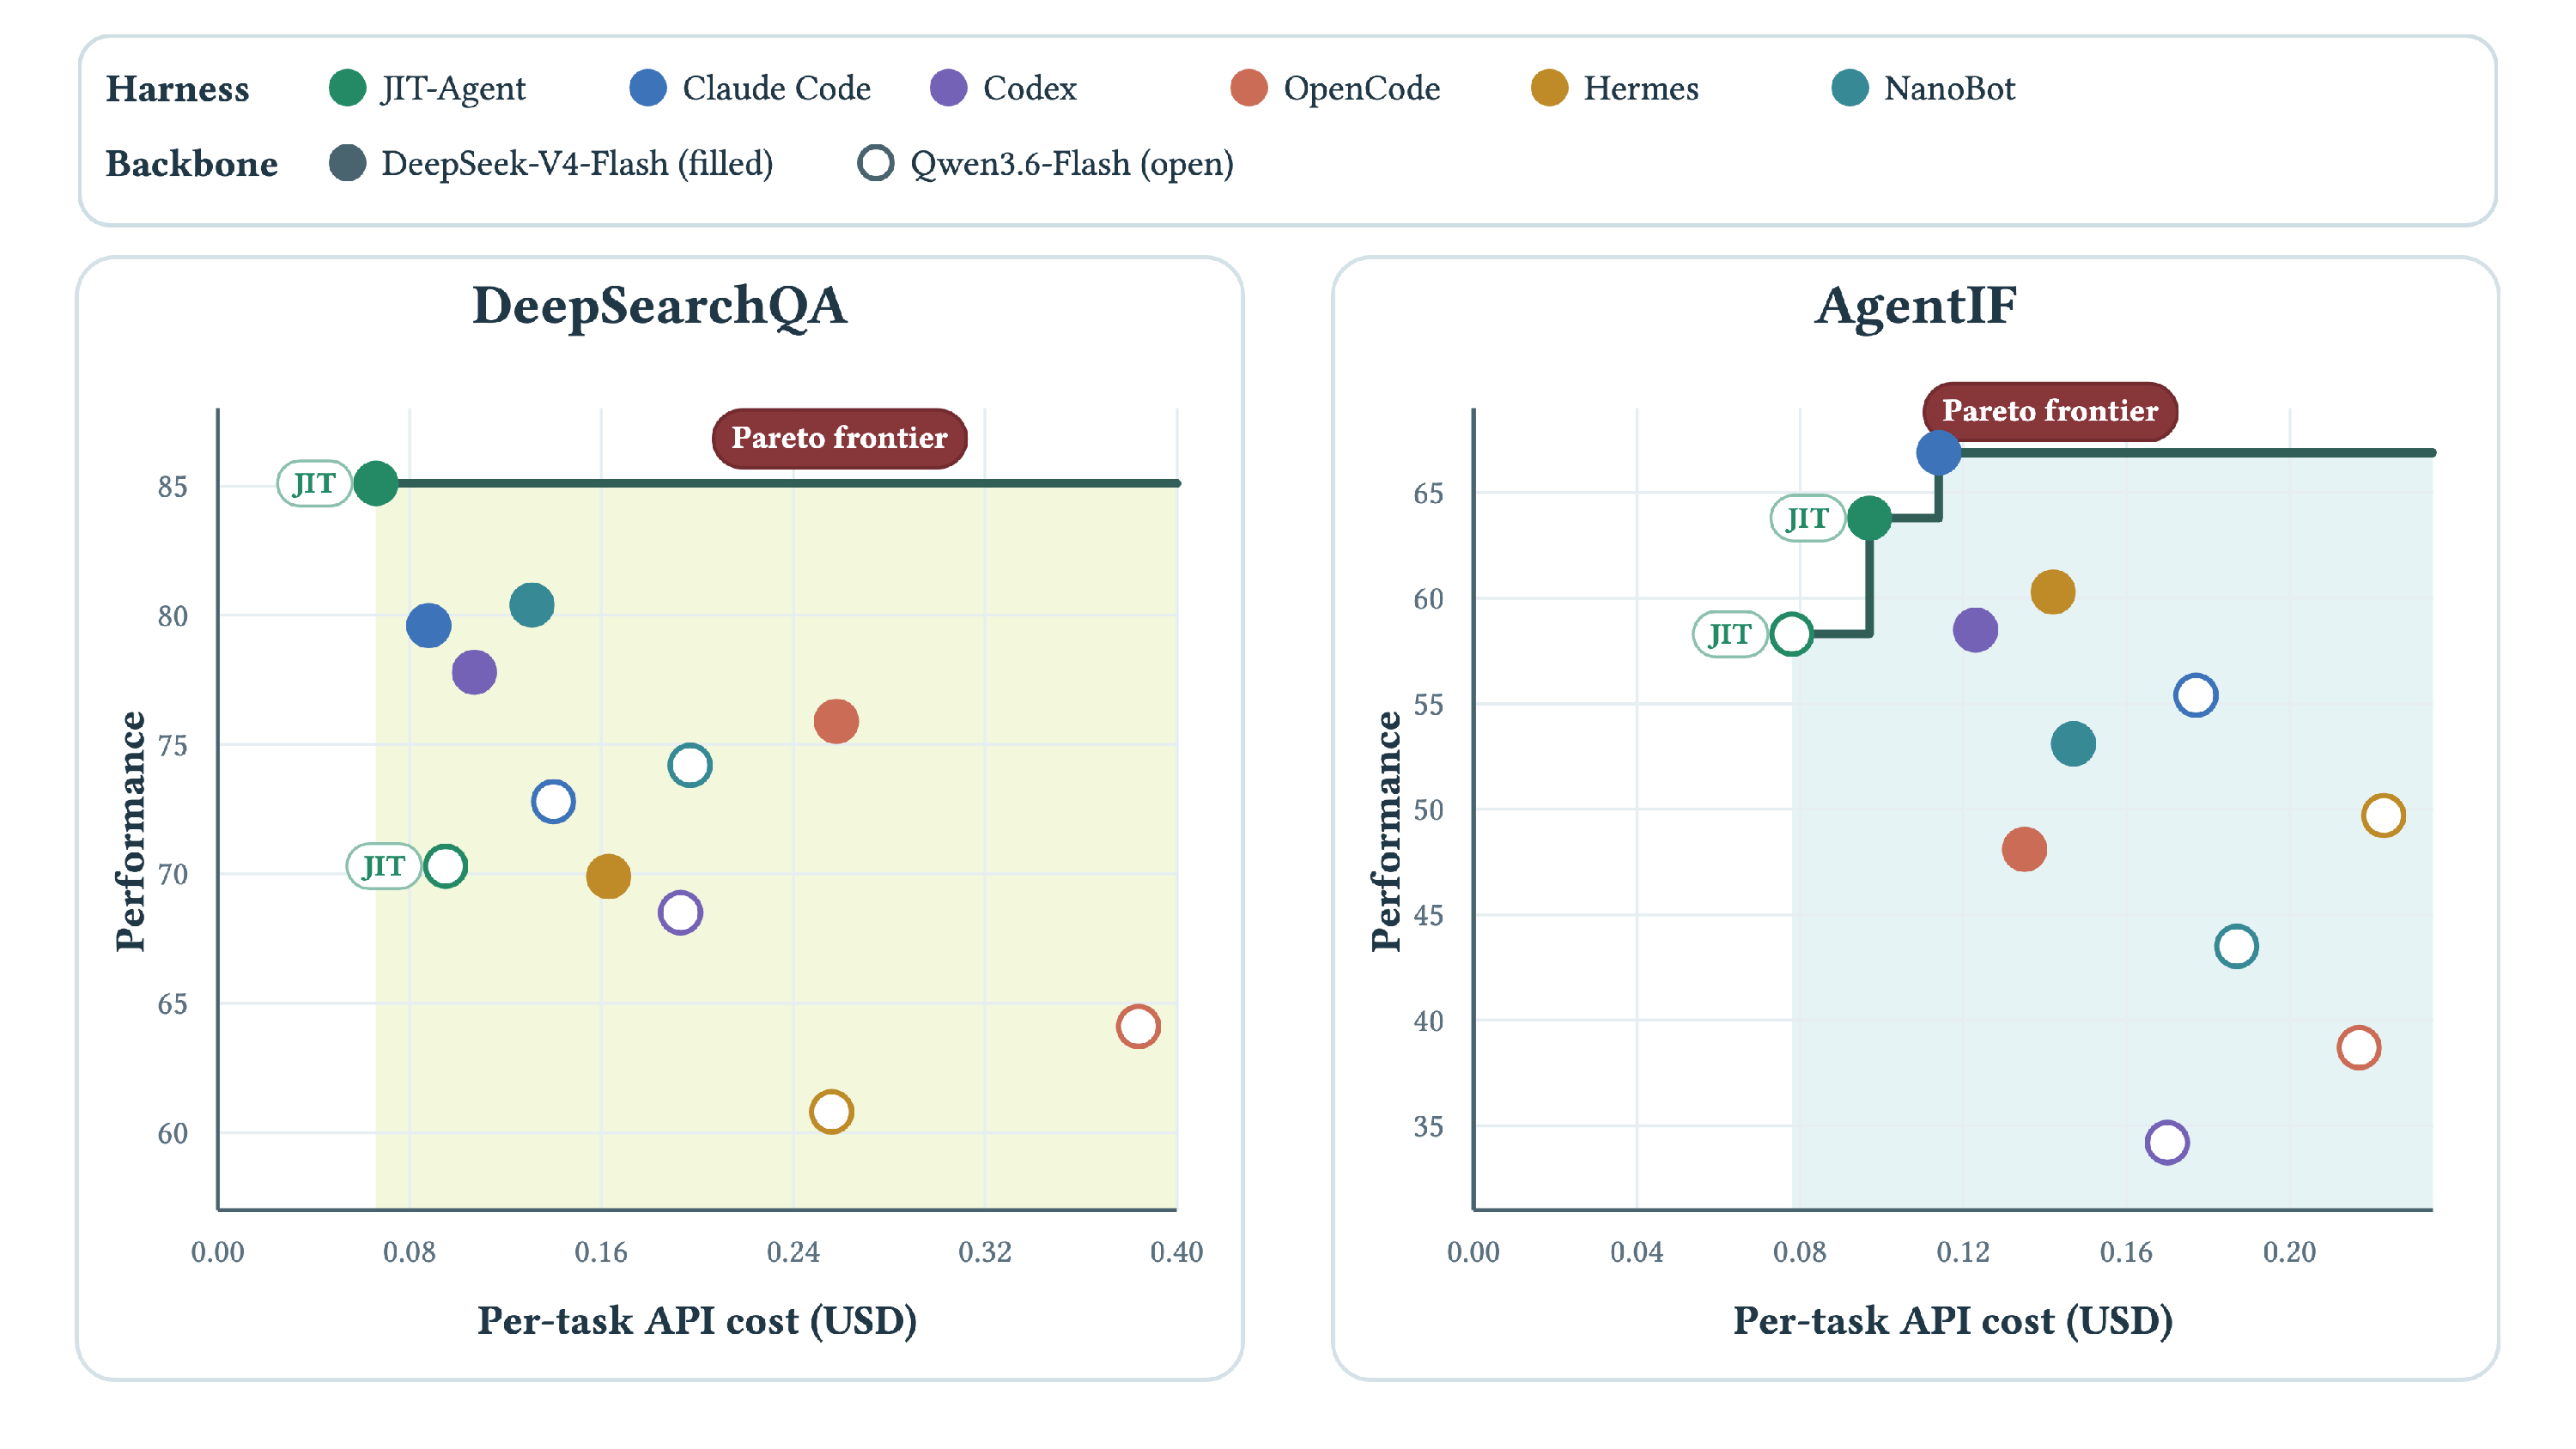
\includegraphics[width=0.85\linewidth]{figures/advanced_harness_cost_performance_dsqa_agentif.pdf}
    \caption{\textbf{DeepSearchQA 与 AgentIF 上的成本--性能权衡。}
    标记颜色表示支架，实心与空心圆分别表示 DeepSeek-V4-Flash 和 Qwen3.6-Flash。横轴为每个样例的 API 成本（美元），纵轴为任务性能。深绿色阶梯线勾勒全局 Pareto 前沿；浅黄绿色和蓝绿色区域中的组合至少被一个 Pareto 最优点支配。}
    \label{fig:pareto_frontiers}
\end{figure}


\subsection{成本--性能 Pareto 前沿}
\label{sec:pareto_frontier}

\Cref{fig:pareto_frontiers} 可视化了 DeepSearchQA 和 AgentIF 受控比较中的成本--性能几何。每个点都是\Cref{tab:advanced_harness_comparison} 中的一个骨干--支架组合；越接近左上角的点越优。
在 DeepSearchQA 上，DeepSeek-V4-Flash + \ourmethod 是所评测组合中一个强 Pareto 最优运行点：每个样例成本为 $\$0.066$ 时得分 $85.1$。与最强固定支架 NanoBot 相比，它提高 $4.7$ 分，同时将成本降低 $49.6\%$（$\$0.131\!\rightarrow\!\$0.066$）。对于 Qwen3.6-Flash，生成支架提供了计算量更低的运行点：它以 $\$0.095$ 的成本得到 $70.3$ 分；NanoBot 则以 $\$0.197$ 的成本得到 $74.2$ 分，即以 $3.9$ 分为代价将成本降低 $51.8\%$。
AgentIF 呈现出不同但互补的前沿。在 DeepSeek-V4-Flash 上，\ourmethod 相较 Claude Code 将成本降低 $14.9\%$（$\$0.097$ 对 $\$0.114$），同时性能仅低 $3.1$ 分（$63.8$ 对 $66.9$）；因此二者均位于前沿。在 Qwen3.6-Flash 上，\ourmethod 严格支配所有固定支架：它将最佳分数从 $55.4$ 提升至 $58.3$，同时把观测到的最低成本从 $\$0.170$ 降至 $\$0.078$。因此，该前沿依赖任务；但 JIT 点一致向左移动表明，任务适应型支架提高了推理效率，而非通过更长轨迹购买准确率。



\subsection{跨模型对的泛化}
\label{sec:model_pair_generalization}

为检验 JIT 支架生成能否跨模型家族与变体迁移，我们评测了覆盖三组模型对的六个骨干模型：DeepSeek-V4-Flash/Pro、Qwen3.6-Flash/Plus 和 Mimo-V2.5-Flash/Pro。对于每个骨干模型，我们固定模型，并在 DeepSearchQA、AgentIF-Oneday、DeepPlanning-Shopping 和 OfficeBench 上比较其标准 ReAct 支架与 JIT 生成的支架。

\begin{figure}[!t]
    \centering
    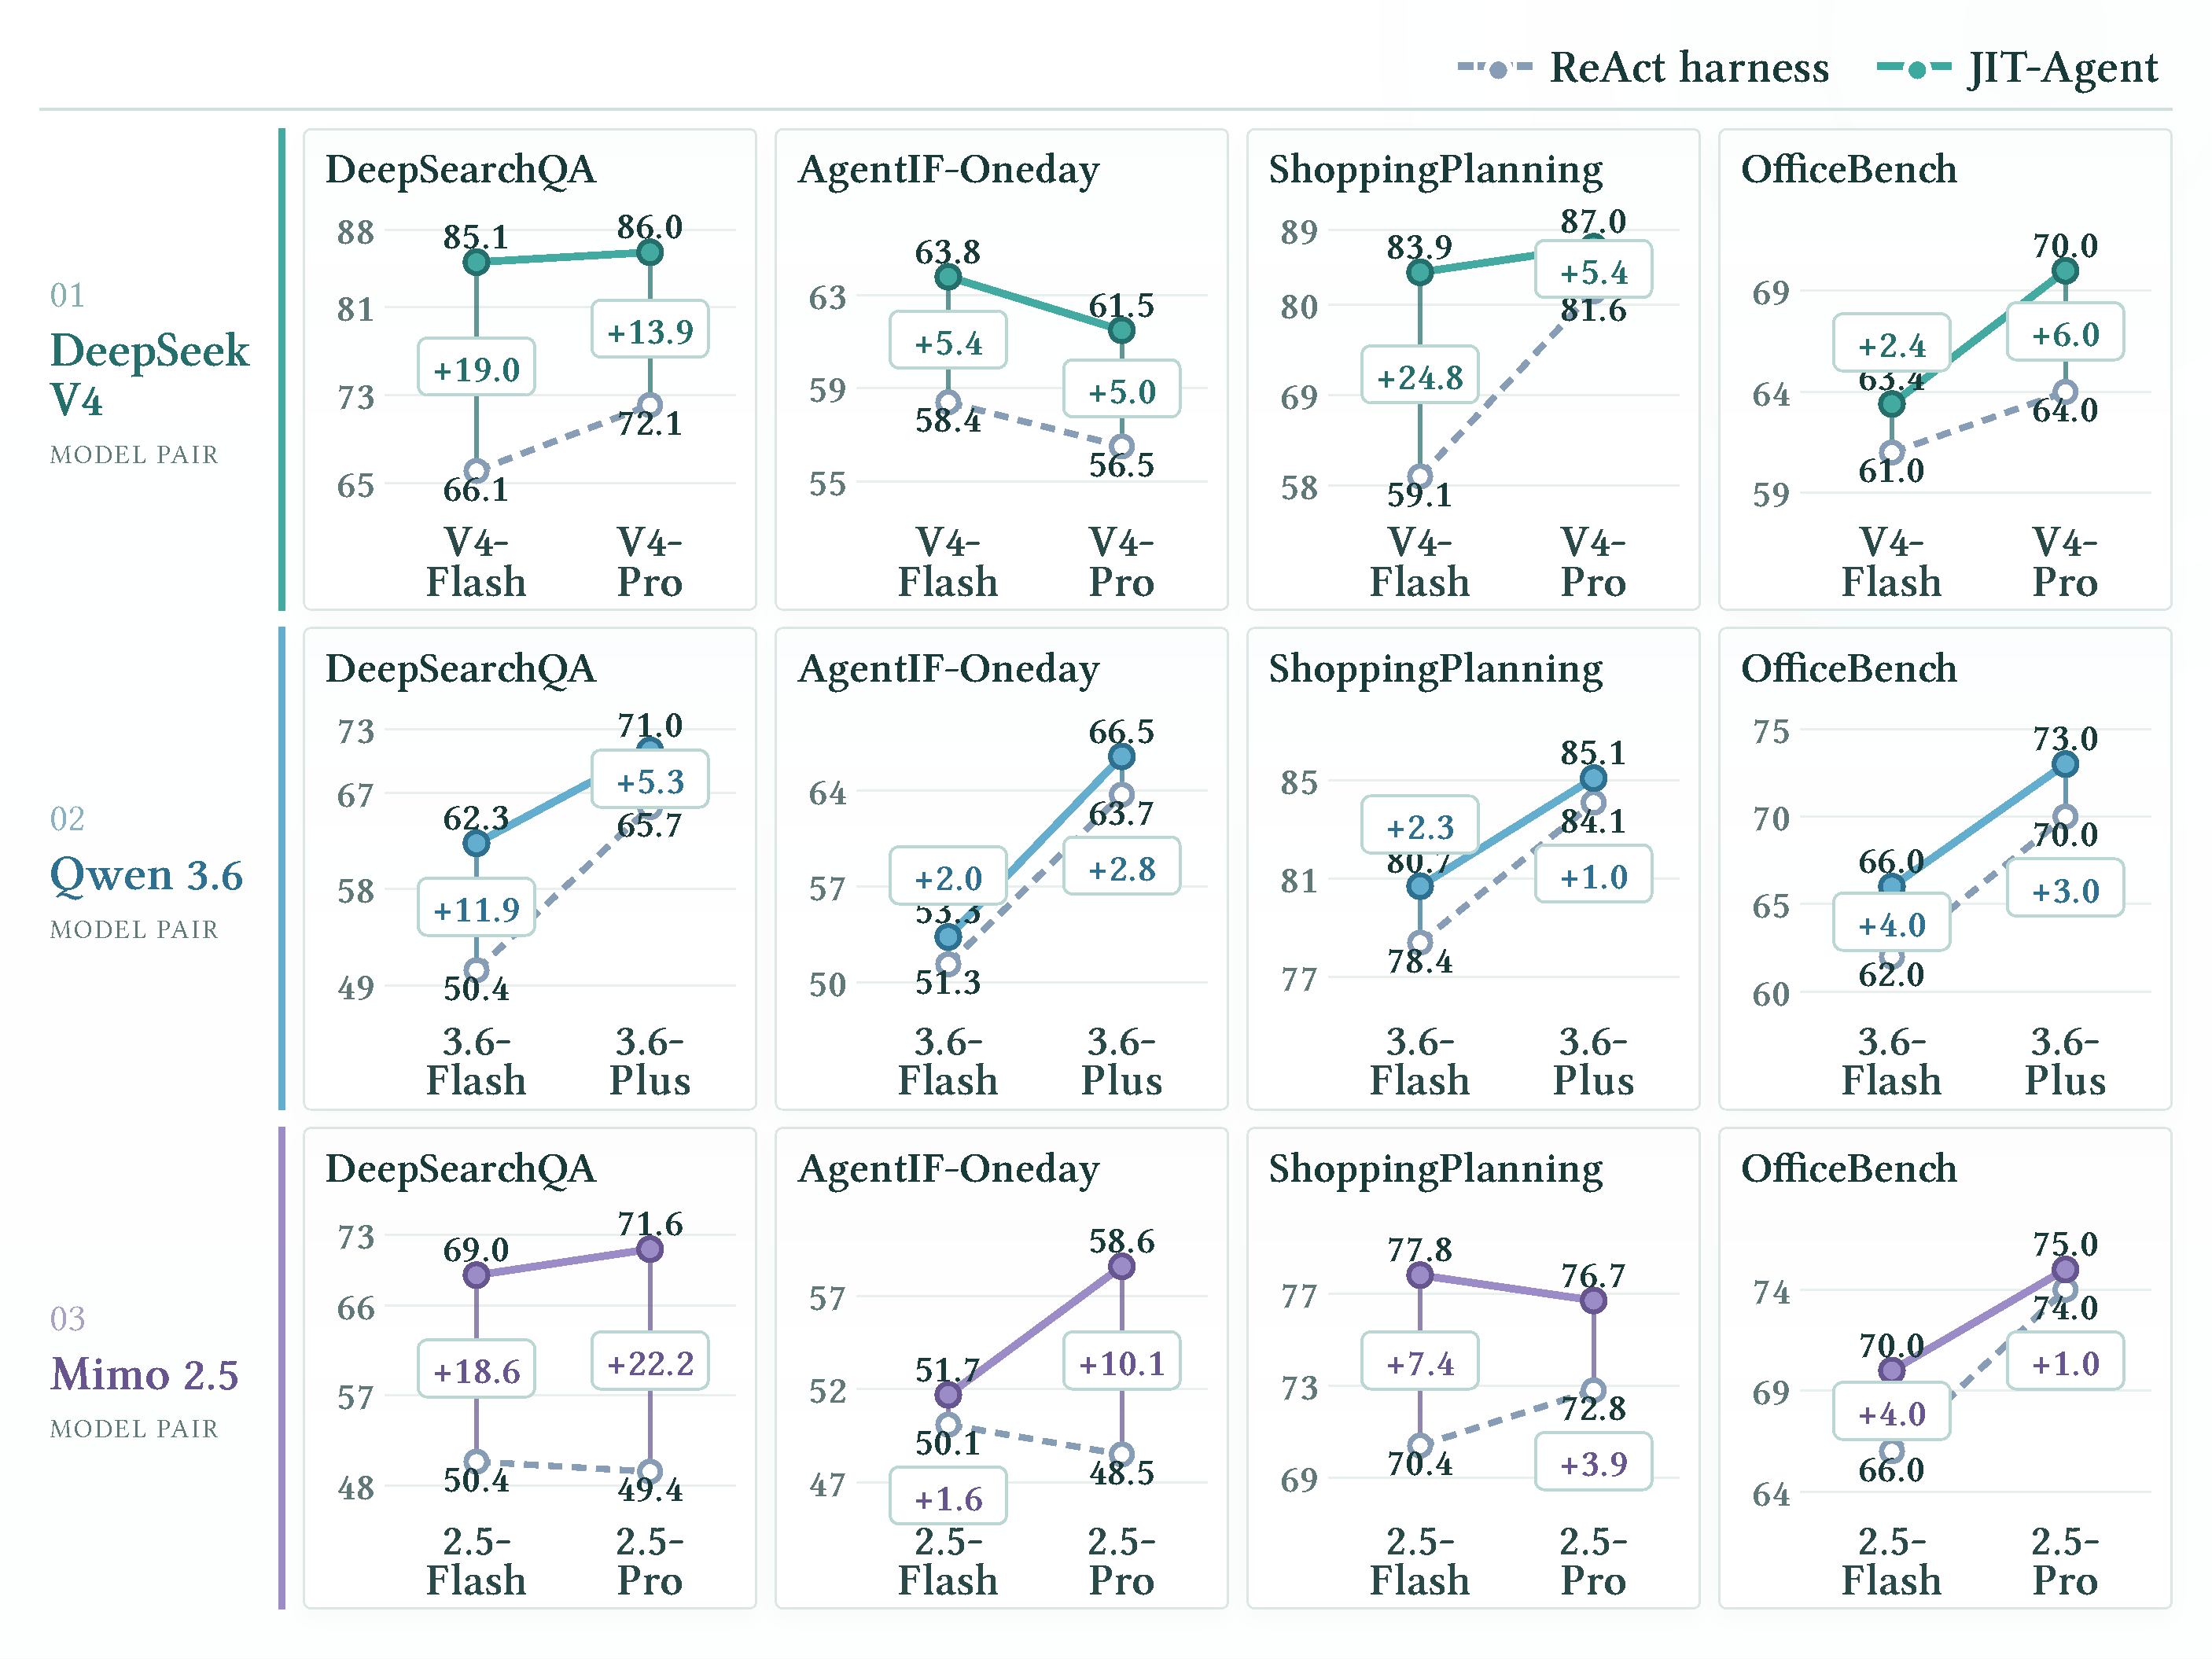
\includegraphics[width=\textwidth]{figures/model_pair_jit_vs_react.pdf}
    \caption{\textbf{JIT 生成的支架相较 ReAct 持续改善成对骨干模型。}
    各行对应三个模型家族及每个家族中的两个变体；各列分别对应 DeepSearchQA、AgentIF-Oneday、DeepPlanning-Shopping 和 OfficeBench。每个面板都比较同一骨干模型使用固定 ReAct 支架（虚线）和 JIT 生成支架（实线）时的结果，标注给出绝对分数增益。DeepSearchQA 使用含 100 个样例的子集；其余三个基准使用含 50 个样例的子集。}
    \label{fig:model_pair_jit_vs_react}
\end{figure}

在全部 24 个直接匹配的骨干--基准比较中，JIT 生成的支架均优于 ReAct，平均提高 $7.6$ 分。该效果对每个家族及每组模型对中的两个变体都成立：DeepSeek V4、Qwen 3.6 和 Mimo 2.5 的平均增益分别为 $10.2$、$4.0$ 和 $8.6$ 分。DeepSearchQA 的平均增益最大，达到 $15.2$ 分，其中 Mimo-V2.5-Pro 和 DeepSeek-V4-Flash 分别提高 $22.2$ 和 $19.0$ 分；DeepPlanning-Shopping 平均提高 $7.5$ 分，其中 DeepSeek-V4-Flash 提高 $24.8$ 分。这些在同一骨干模型内的一致增益表明，支架智能能够跨模型家族和变体迁移，而非仅仅弥补某一特定骨干模型的不足。


\subsection{测试时支架演化}
\label{sec:test_time_evolution}

\ourmethod 不仅用于一次性生成支架，还会根据执行反馈改进其档案。我们比较了支架生成彼此独立的\emph{静态 JIT}，以及在整个评测流中持续检索和更新支架的\emph{流式 JIT}。

\begin{figure}[!t]
    \centering
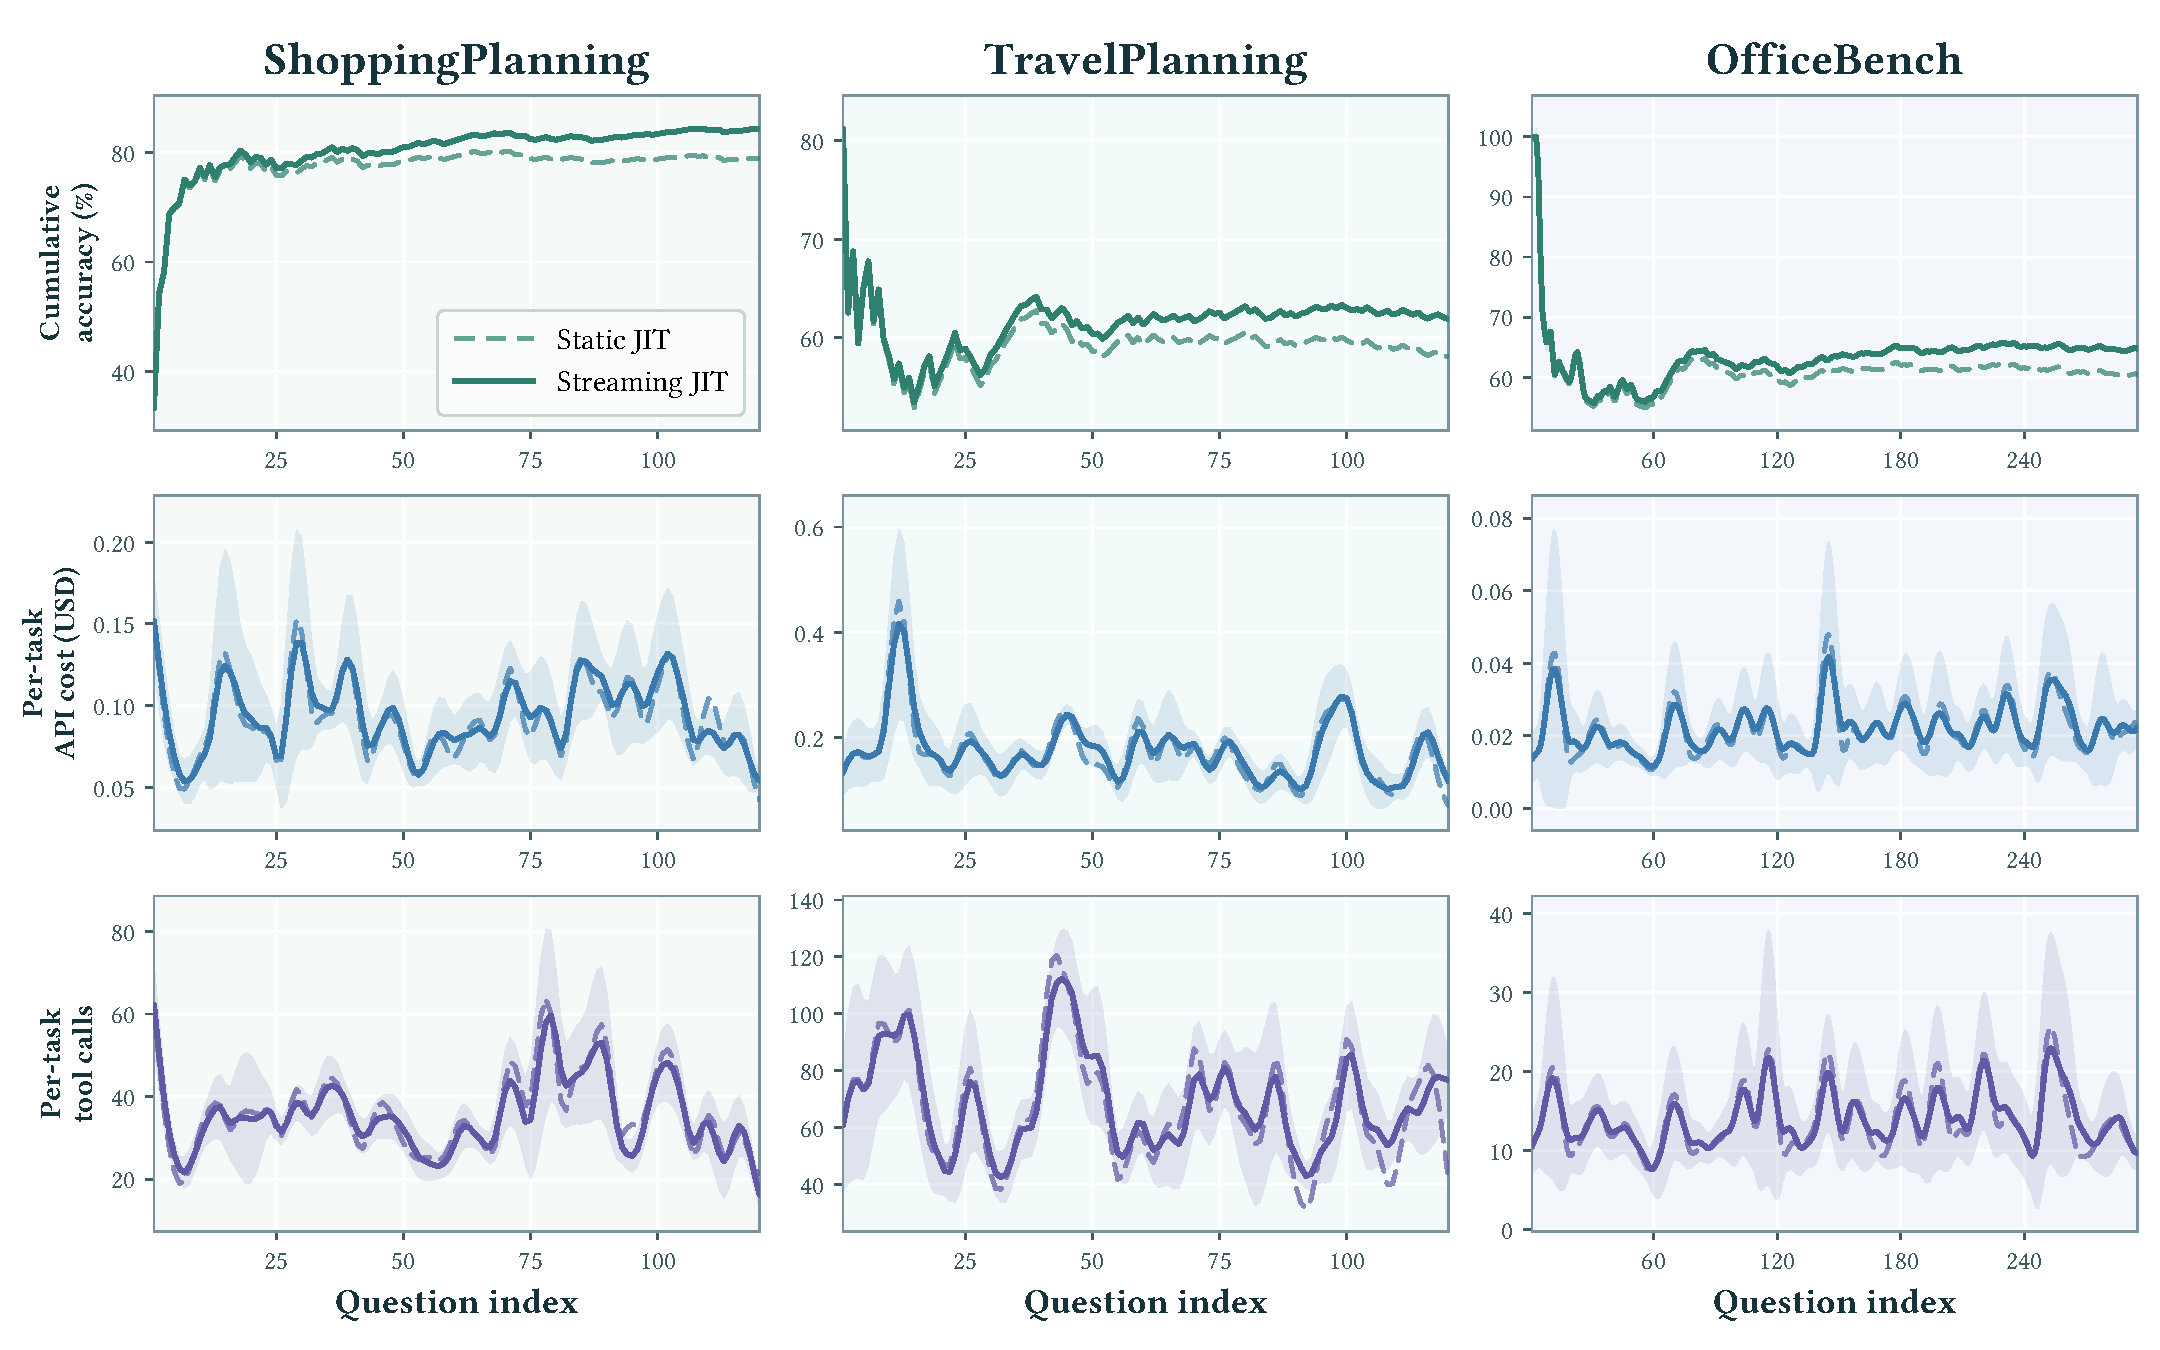
\includegraphics[width=\linewidth]{figures/jit_growth_curves_streaming_comparison_.pdf}
\caption{\textbf{跨任务流的流式测试时支架演化。}
图中给出 DeepPlanning-Shopping、DeepPlanning-Travel 和 OfficeBench 上的累积准确率（上）、每任务 API 成本（中）和每任务工具调用次数（下）。虚线表示静态 JIT，其中任务专用支架的生成彼此独立；实线表示流式 JIT，它会随着新任务到来持续吸收执行反馈。阴影区域表示流式轨迹周围的局部变化。流式 JIT 在三个基准结束时都获得更高的累积准确率，而 API 成本与工具使用轨迹仍依赖具体任务，且总体量级相近。}
    \label{fig:test_time_harness_evolution}
\end{figure}

流式 JIT 在 DeepPlanning-Shopping、DeepPlanning-Travel 和 OfficeBench 上的最终结果均高于静态变体。在三个任务流中，累积准确率优势都随着执行反馈的积累而出现，并一直保持到评测结束。相应的成本和工具调用轨迹表明，最终收益并非都与更大的交互预算绑定。这一模式符合 Evo-GDPO 的目标：只有推进档案前沿的支架才会被保留。


\subsection{生成支架的可视化}
\label{sec:harness_visualization}
定量结果已经表明，生成的支架能够改善执行；接下来我们考察 \ourmethod 实际生成的内容。图~\ref{fig:harness-palimpsest} 和图~\ref{fig:harness-trapdoor} 可视化了在同一四模块协议下，为计算结构截然不同的任务生成的两个支架。二者的差异不止在于提示或模块名称：生成的规划表示、动作拓扑、持久状态和暴露能力都围绕每项任务的需求重新组织。

\begin{figure}[!tpb]
    \centering
    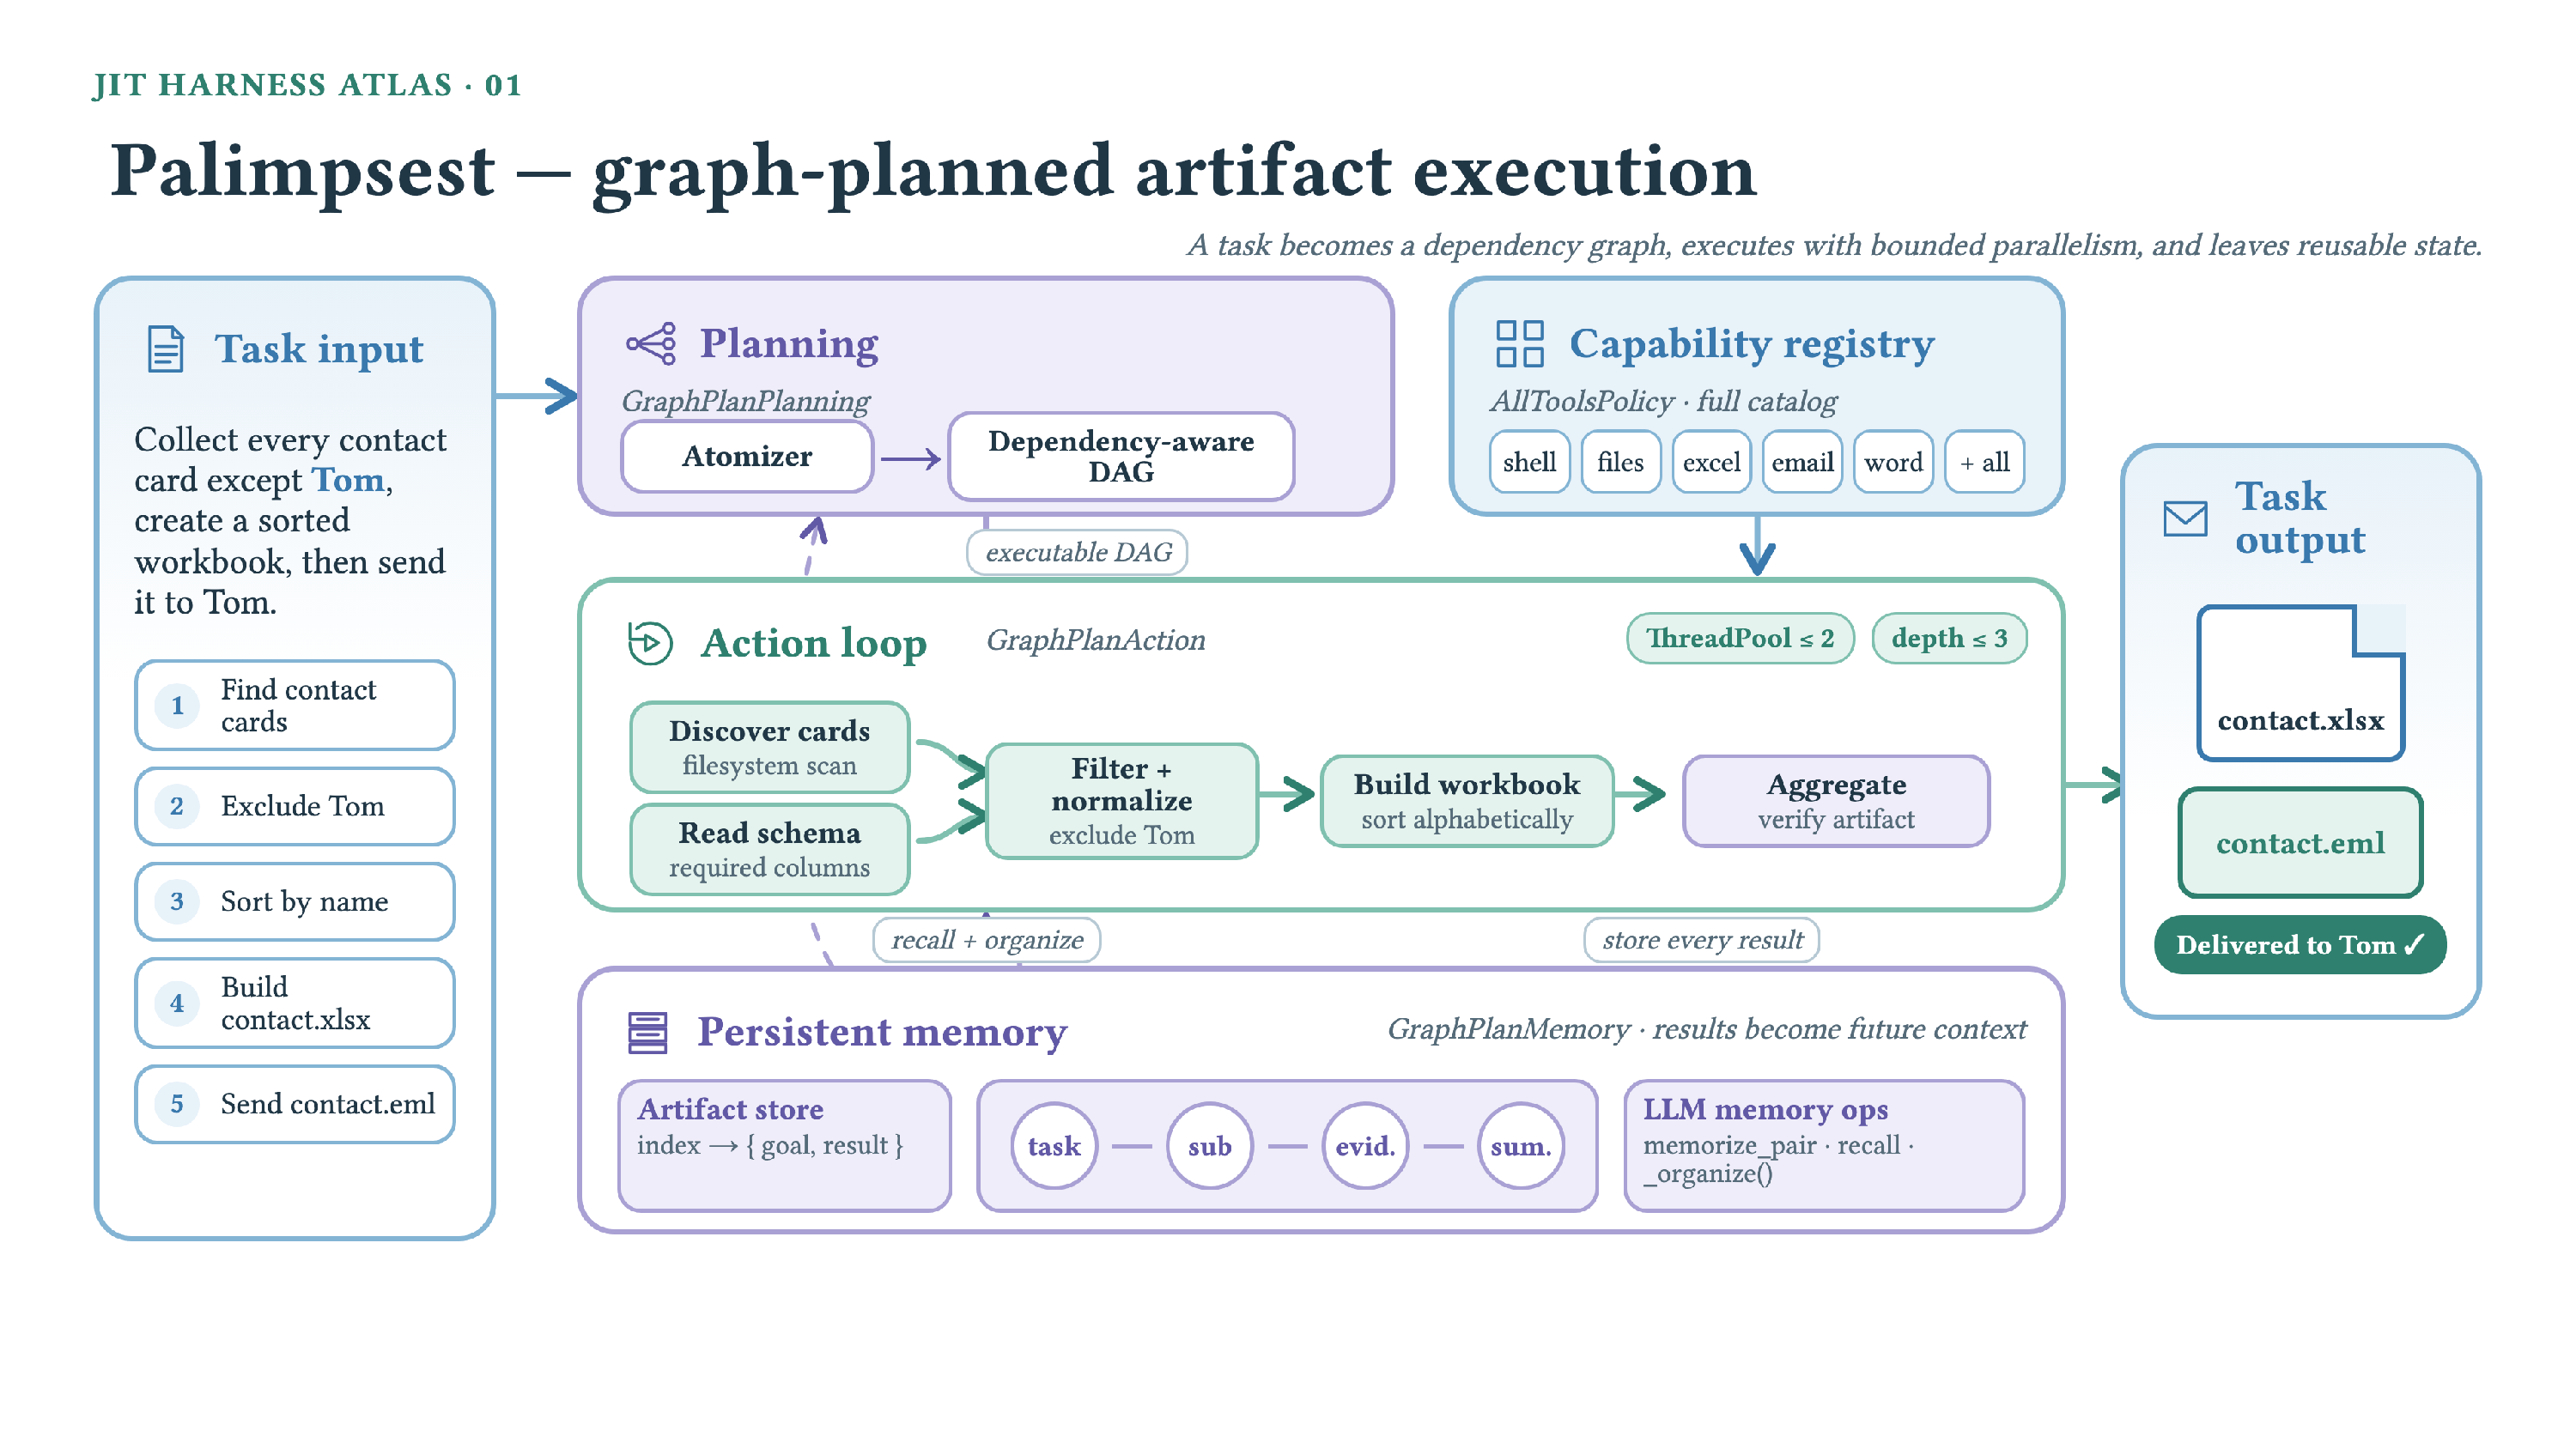
\includegraphics[width=\textwidth]{figures/harness_atlas_reworked/palimpsest_flow.pdf}
    \vspace{-4em}
    \caption{\textbf{Palimpsest：由图规划的工件执行。}\texttt{GraphPlanPlanning} 将联系人处理请求转化为 DAG；\texttt{GraphPlanAction} 以有界宽度和深度执行该图，而 \texttt{GraphPlanMemory} 存储可复用工件和推理状态。}
    \label{fig:harness-palimpsest}
    \end{figure}

\paragraph{把工件生产表示为依赖图。}
\textsc{Palimpsest} 面向一项跨应用任务生成；该任务必须发现联系人卡片、排除一个人、对其余记录进行规范化和排序、创建工作簿，并通过电子邮件交付。支架把这些要求编译为显式 DAG：发现与模式检查为筛选提供前置条件，工作簿构建等待规范化记录，而交付则等待工件验证。随后，\texttt{GraphPlanAction} 以有界宽度和深度执行就绪节点；\texttt{GraphPlanMemory} 则为中间目标、证据和工件建立索引，使下游节点能够直接使用已完成结果，而无需从交互记录中重建它们。所得支架匹配任务的工件依赖与提交顺序，把冗长的自然语言请求转化为可验证的生产流水线。

\begin{figure}[!tpb]
    \centering
    \vspace{-0.2em}
    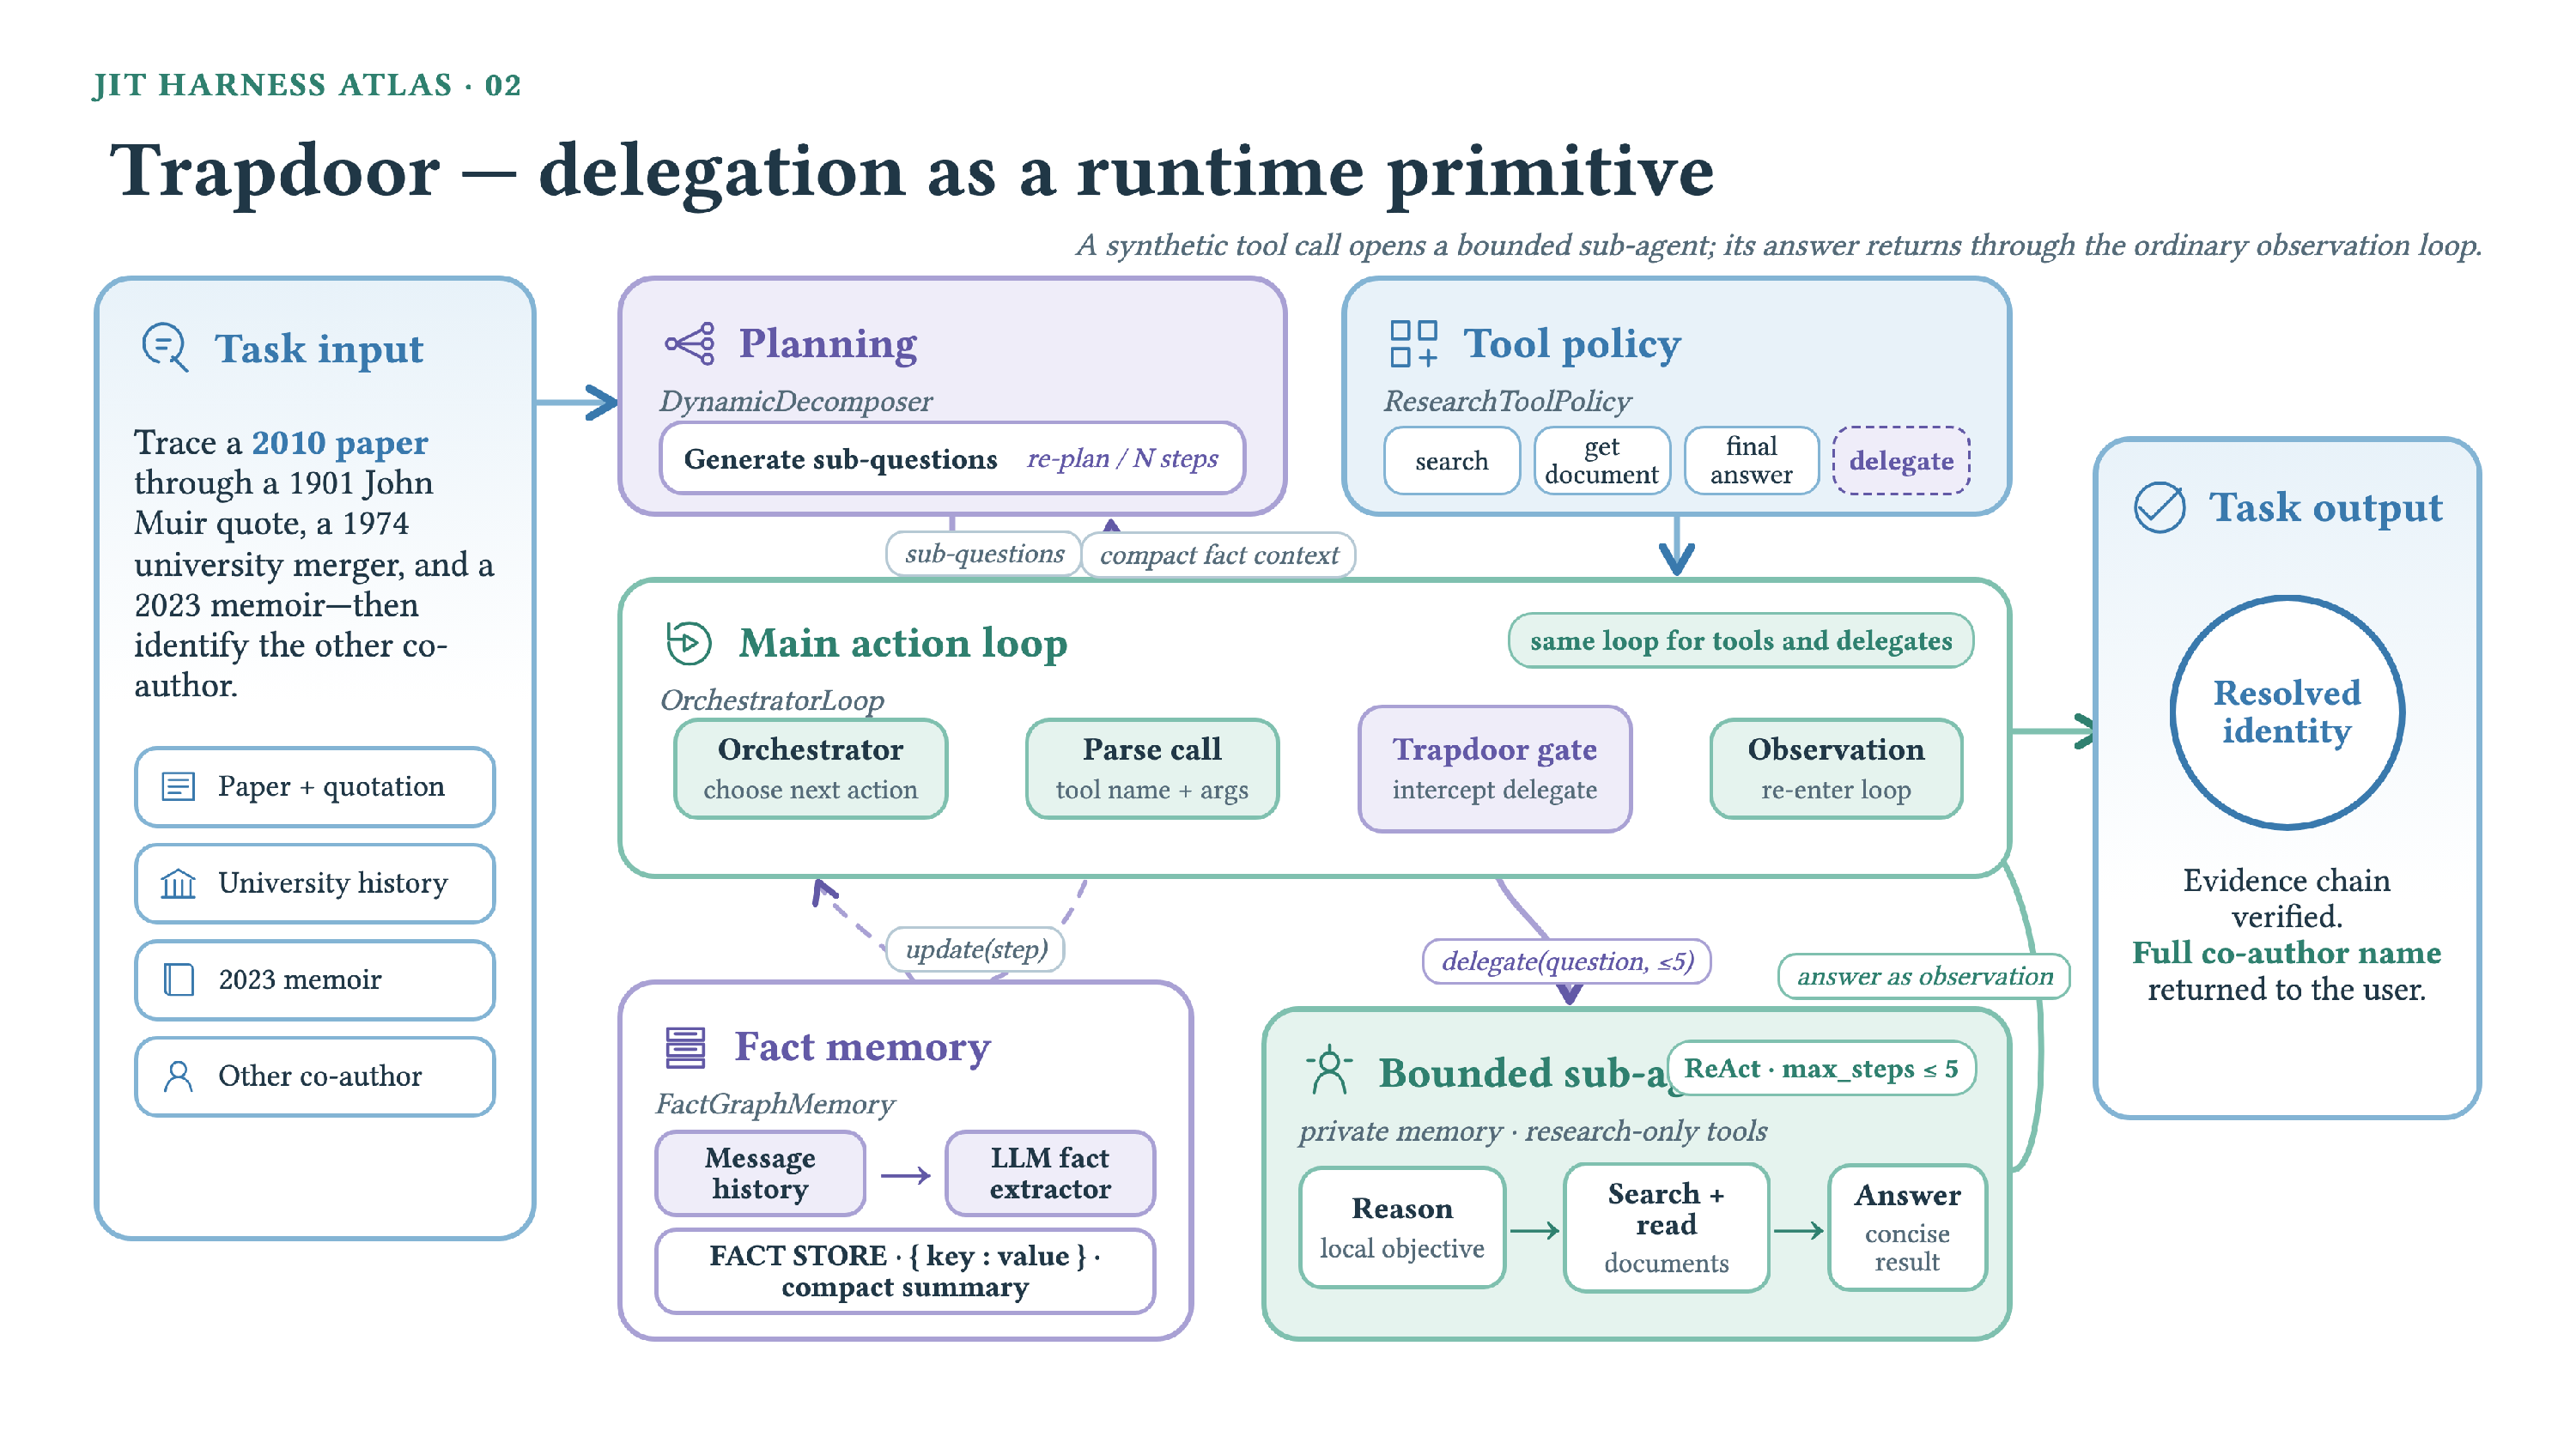
\includegraphics[width=\textwidth]{figures/harness_atlas_reworked/trapdoor_flow.pdf}
    \vspace{-2em}
    \caption{\textbf{Trapdoor：委派工具调用背后的有界研究。}合成的 \texttt{delegate} 能力由 \texttt{OrchestratorLoop} 截获；后者运行有界子智能体，并把提取的事实写入 \texttt{FactGraphMemory}。}
        \label{fig:harness-trapdoor}
\end{figure}

\paragraph{把深度研究表示为有界递归委派。}
\textsc{Trapdoor} 处理一个多跳身份问题，其线索横跨一段历史引文、一次大学合并、一本回忆录和一篇研究论文。固定 DAG 会过早承诺一条尚不确定的证据路径，因此生成的支架使用 \texttt{DynamicDecomposer} 形成并修订子问题，并在研究工具策略中增添合成的 \texttt{delegate} 能力。一次 \texttt{delegate} 调用会打开私有研究子智能体；该子智能体拥有自己的记忆、仅限研究的工具及五步预算，返回的答案再作为普通观察进入父循环。与此同时，\texttt{FactGraphMemory} 从不断增长的历史中提取紧凑的键--值事实，使父智能体无需继承每条子智能体轨迹，就能整合各分支证据。因此，对于不确定性需要通过分支式证据收集来解决的任务，该支架专门把递归研究变成一种运行时原语。

这种对比构成了核心定性结果：同一个生成器把一项任务映射为带工件存储的图执行，把另一项任务映射为带事实存储的递归编排。共享协议约束的是接口，而非行为。附录~\ref{sec:additional_harness_visualizations} 中的其他案例把这一模式扩展到层次化上下文折叠、完成度门控的工具访问、阶段条件化执行、证据矩阵搜索、选择性上下文渲染、有类型计算状态、逐文件确定性验证及局部动作修复；其流程见图~\ref{fig:harness-origami}--\ref{fig:harness-mulligan}。

\section{结论与未来工作}

\paragraph{结论。}
我们提出了 \ourmethod，一种专门在推理时合成、修复和演化任务条件化智能体支架的模型。通过用可组合四模块协议表示支架，并借助定制学习、修复监督和 Evo-GDPO 训练生成器，\ourmethod 把支架构建从人工工程化的预先工件转化为学习所得能力。在深度研究、日常工作、规划和工作区任务上，JIT 生成的支架持续增强其底层骨干模型，与前沿模型和先进固定支架竞争，并改善成本--性能权衡。这些结果确立了支架智能，也就是适配模型赖以行动的运行脚手架的能力；它是超越模型权重本身、可训练且可迁移的智能体能力来源。

\paragraph{未来工作。}
我们把支架智能视为与模型容量和推理算力并列的另一个基础扩展维度，并将 \ourmethod 视为实现这一愿景的一步。长期机遇在于模型--支架协同设计范式：基础模型与塑造其记忆、规划、动作和工具使用方式的运行结构共同训练。尽管如此，我们认为未来系统不必遵循本文刻意探索的激进形式，即整个脚手架均可即时重新设计；生产运行时可以保留稳定核心，同时允许模型在任务需要时构建、修订或替换选定的支架组件。随着这一范式成熟，本文为支架合成、修复与演化开发的能力将越来越多地被基础模型自身内化。届时，模型不仅会学习如何在给定支架内行动，还会学习如何改进其赖以行动的支架，从而围绕适应性接口、可验证运行时修改及模型与执行系统的协同扩展，开启广阔的研究议程。

\section*{贡献者}

\paragraph{项目负责人} Guibin Zhang
\vspace{-0.4em}
\paragraph{核心贡献者} Guibin Zhang, Leo Lu, Fangzhou Xie
\vspace{-0.4em}
\paragraph{贡献者} Kang Zhu, Junhao Wang, Zhifei Xie, Zhaochen Yu, Zihang Liu, Zhongxiang Sun, Qiankun Li, Yue Liao, Heng Chang, Xiaobin Hu, Qibing Ren
\vspace{-0.4em}
\paragraph{通讯作者} Wangchunshu Zhou, Shuicheng Yan

\bibliographystyle{plainnat}
\bibliography{refs}


\clearpage
\appendix
\section{更多生成支架的可视化}
\label{sec:additional_harness_visualizations}
\setcounter{figure}{0}
\renewcommand{\thefigure}{\thesection.\arabic{figure}}
\renewcommand{\theHfigure}{\thesection.\arabic{figure}}
本附录在第~\ref{sec:harness_visualization}~节两个代表性案例的基础上，补充展示同一四模块协议下生成的八个支架。这些样例覆盖约束密集型购物与旅行、分阶段 Web 产品构建、线索驱动研究、证据敏感检索、数值分析和工作区操作。它们并非单一执行模板的不同变体：\ourmethod 会选择适合每项请求结构的状态表示和控制机制，再围绕该选择实例化规划、动作、记忆和能力编排。总体而言，这些案例让任务条件化支架定制在执行语义而非提示措辞层面变得可见。

\begin{figure}[!htbp]
    \centering
    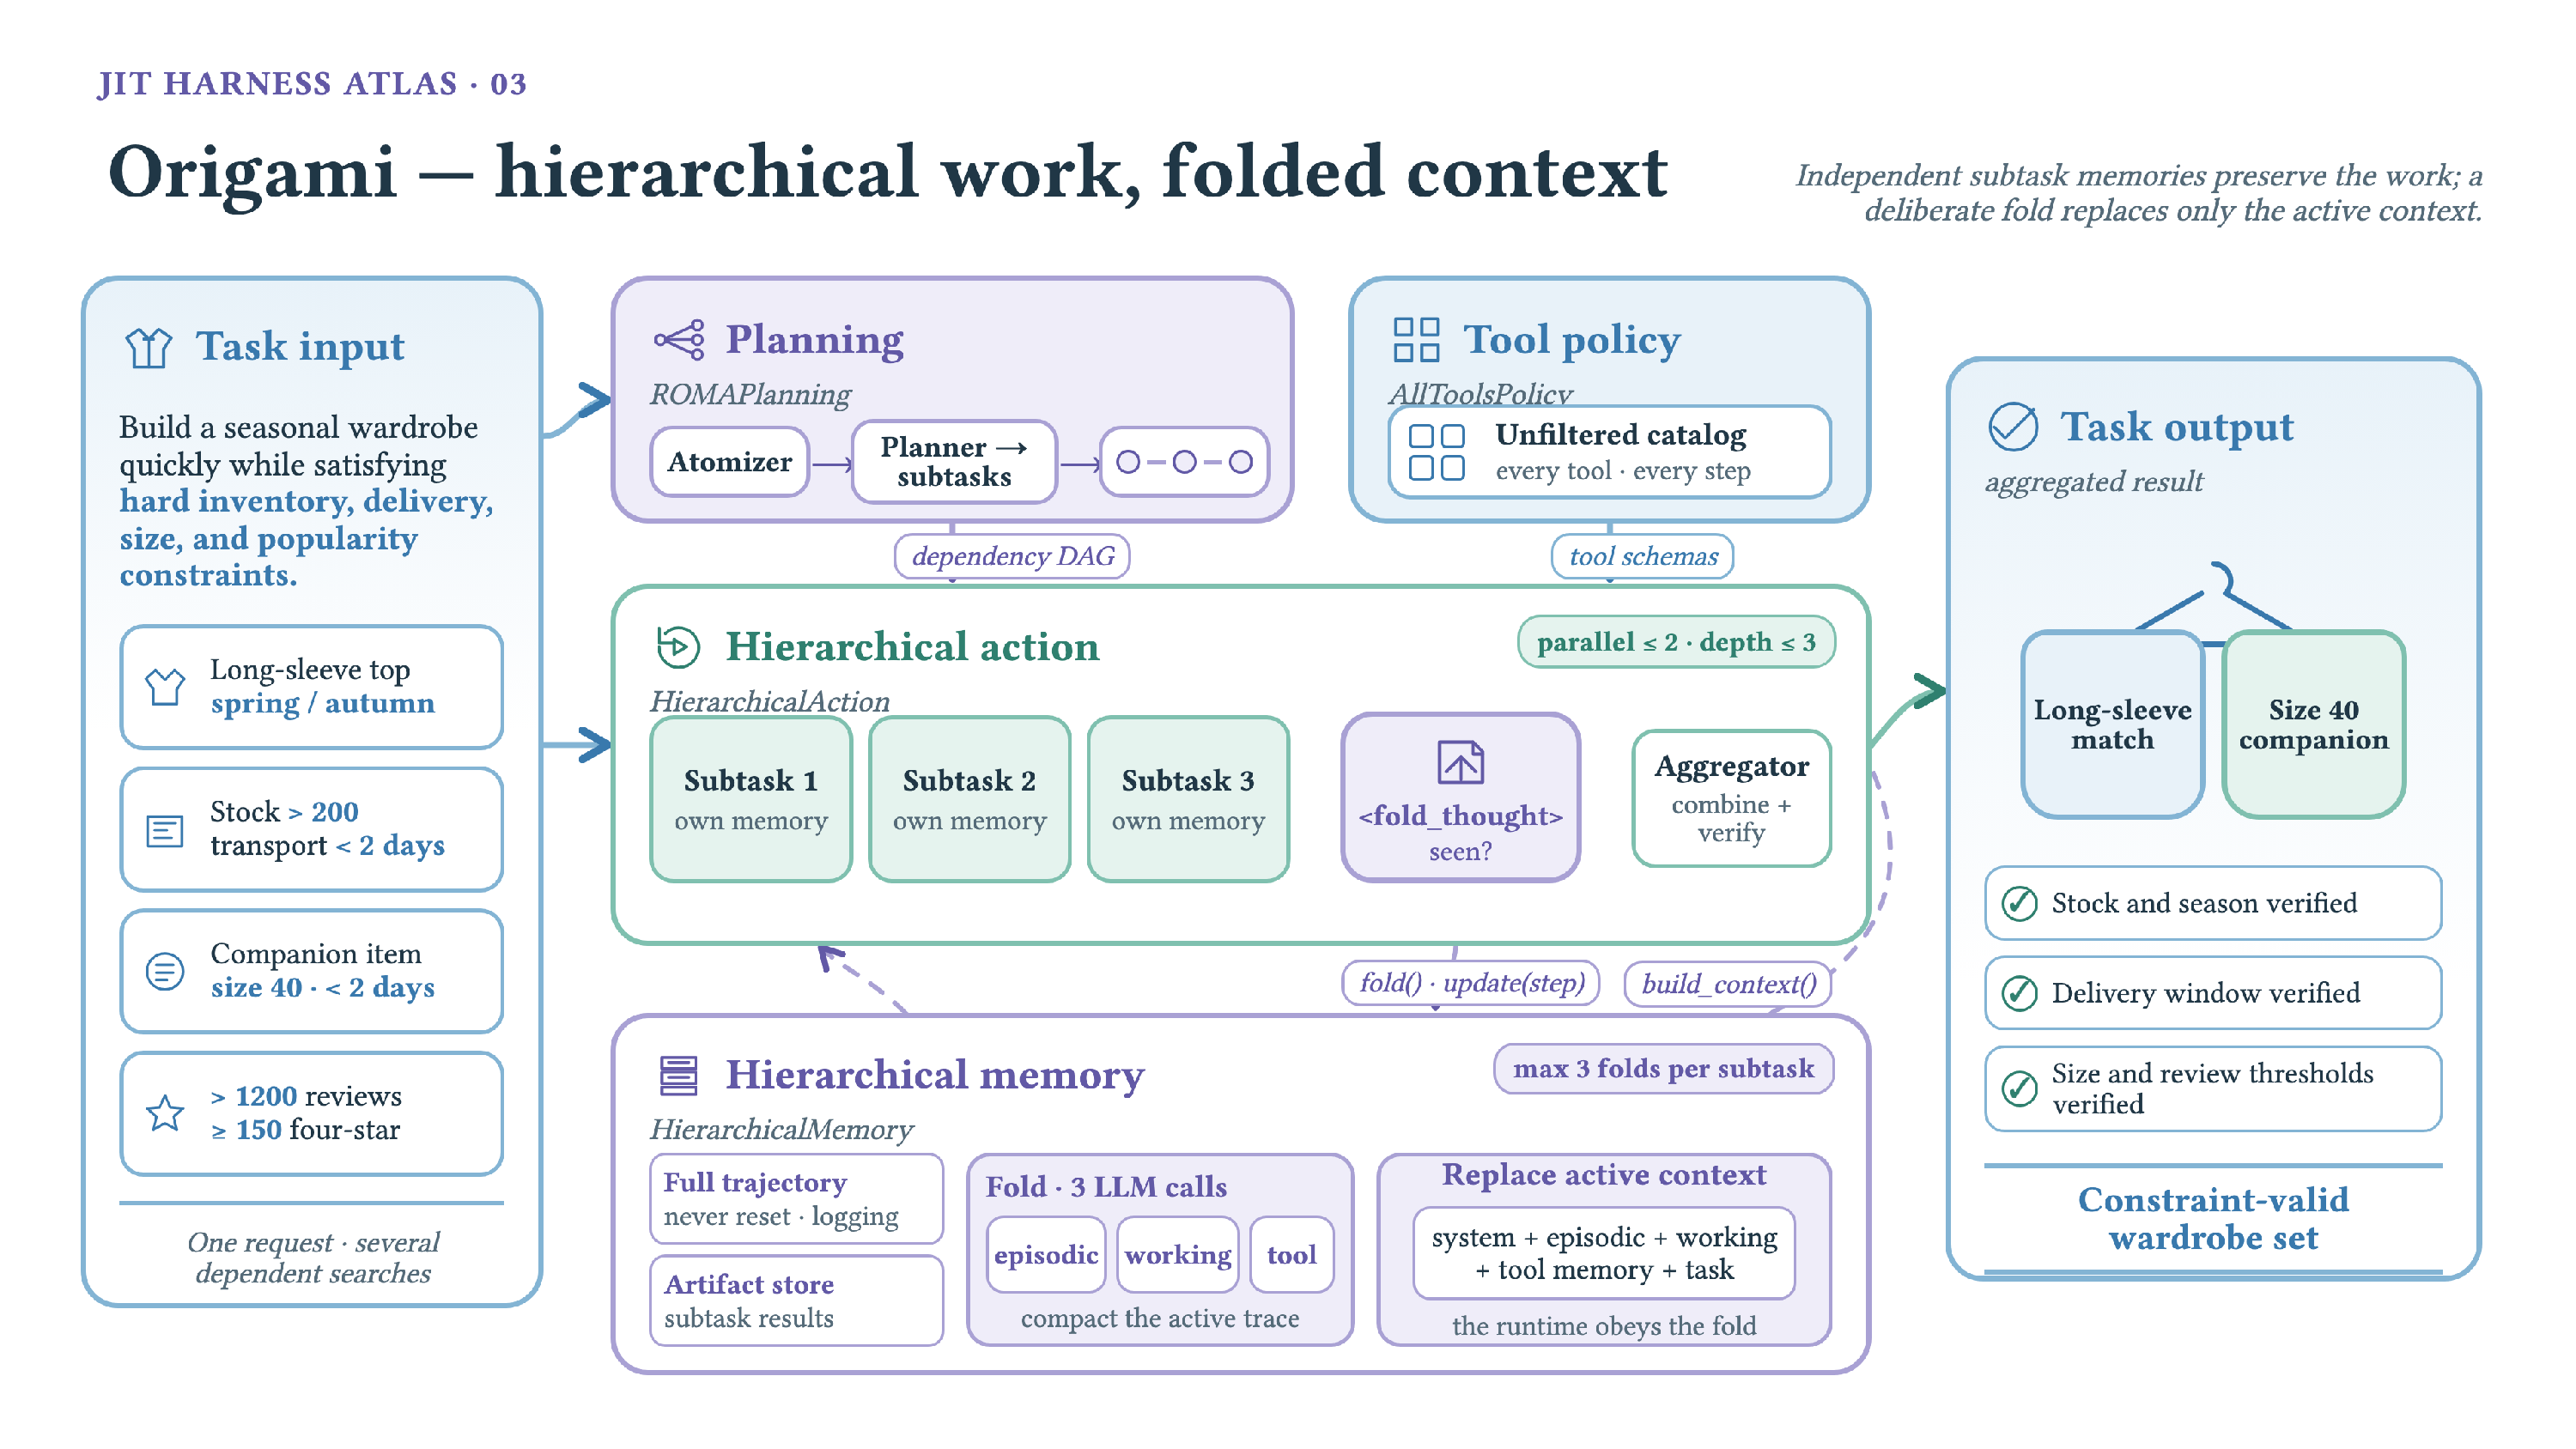
\includegraphics[width=\textwidth]{figures/harness_atlas_reworked/origami_flow.pdf}
    \vspace{-0.55em}
    \caption{\textbf{Origami：使用折叠上下文的层次化工作。}\texttt{ROMAPlanning} 创建隔离的子任务；\texttt{HierarchicalMemory} 保留其轨迹和工件，而 \texttt{fold\_thought} 在聚合前只替换活动工作上下文。}
    \label{fig:harness-origami}
\end{figure}
\begin{figure}[!htbp]
    \centering
    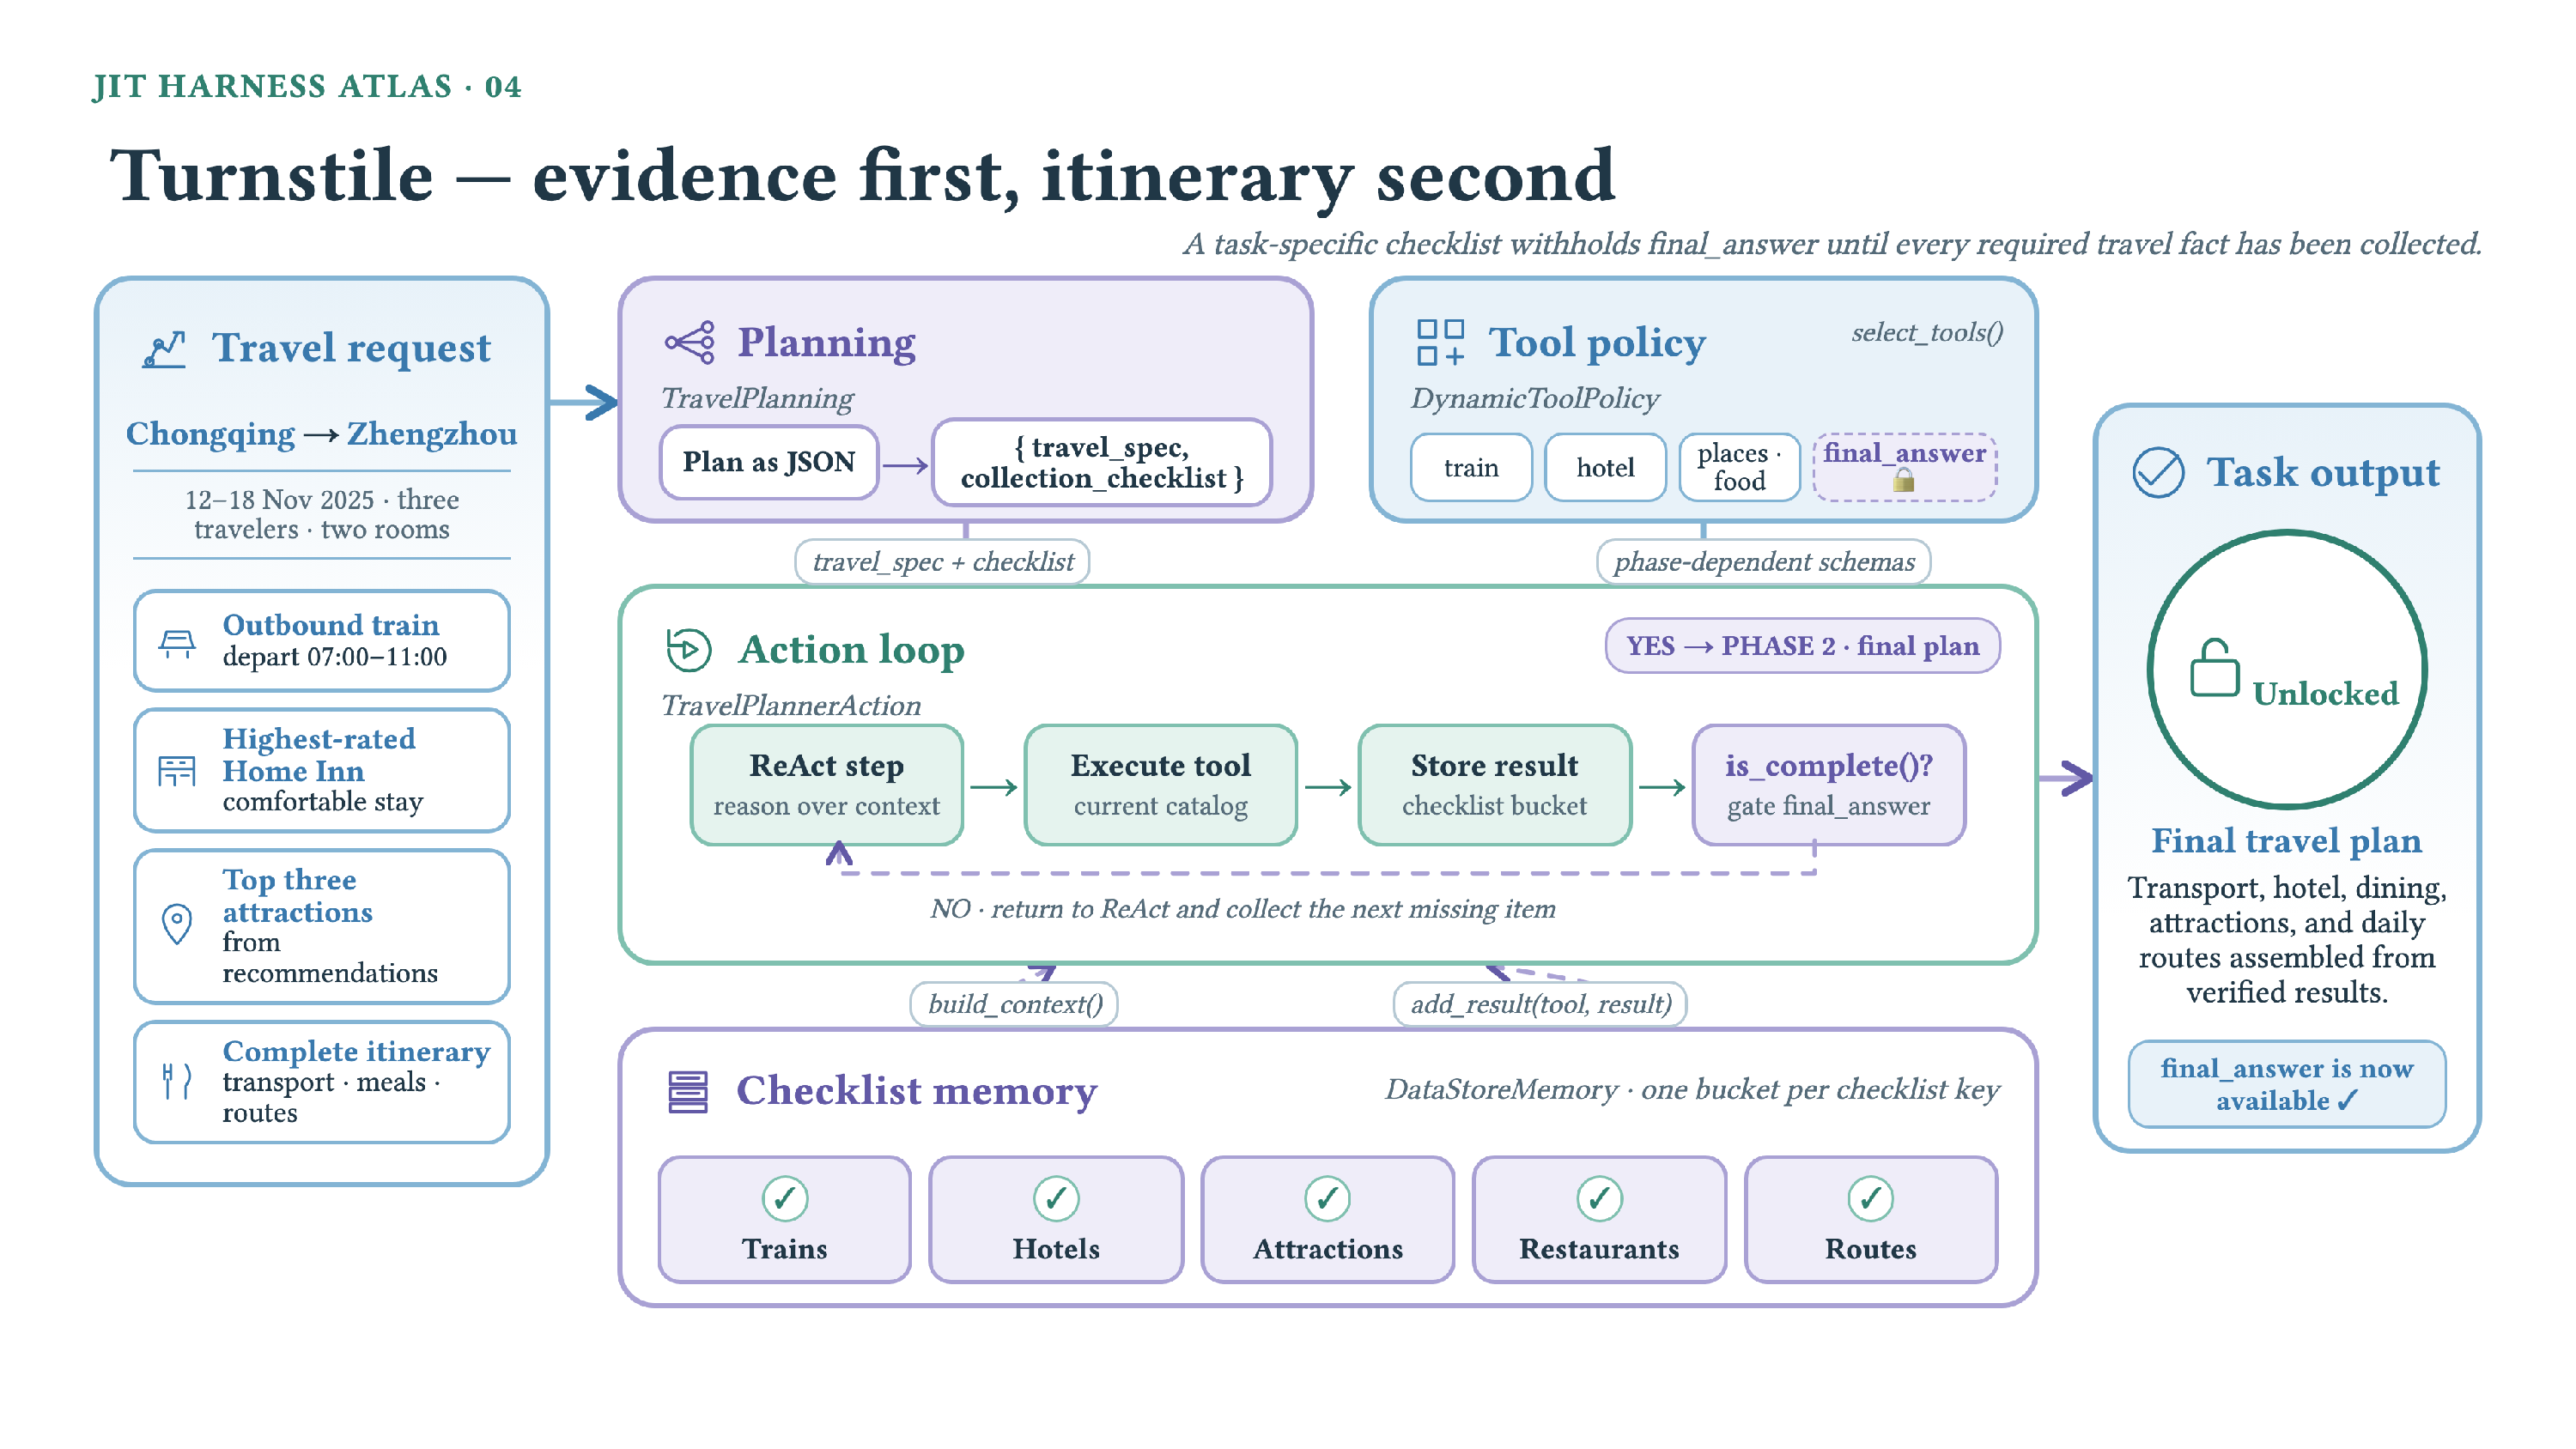
\includegraphics[width=\textwidth]{figures/harness_atlas_reworked/turnstile_flow.pdf}
    \vspace{-0.55em}
    \caption{\textbf{Turnstile：证据优先，行程随后。}\texttt{TravelPlanning} 发出旅行规范和检查清单，\texttt{DataStoreMemory} 跟踪所需证据桶，而 \texttt{DynamicToolPolicy} 只有在 \texttt{is\_complete()} 成功后才暴露 \texttt{final\_answer}。}
    \label{fig:harness-turnstile}
\end{figure}

图~\ref{fig:harness-origami} 和图~\ref{fig:harness-turnstile} 展示了两种通过记忆控制长视野执行的任务专用方式。\textsc{Origami} 必须在库存、交付、尺码、评论数和评分等耦合约束下组合一套应季衣橱。\texttt{ROMAPlanning} 将请求分解为相互依赖的商品搜索，\texttt{HierarchicalAction} 以有界深度并行运行至多两个分支，每个分支保留自己的轨迹和工件。当某个分支变长时，\texttt{fold\_thought} 仅替换其活动工作上下文；已完成子任务的结果仍可用于最终约束检查。因此，该支架把上下文用在组合式购物任务中尚未解决的部分，同时不丢弃早先的商品证据。

相比之下，\textsc{Turnstile} 服务于一项明确日期、乘客、房间、出发时间窗、评分最高酒店、景点、餐食和每日路线的旅行请求。生成的 \texttt{TravelPlanning} 模块把这些义务编译为有类型的 \texttt{travel\_spec} 和收集清单，\texttt{DataStoreMemory} 为每类证据分配专用存储桶。\texttt{DynamicToolPolicy} 暴露用于补齐缺失存储桶的搜索工具，但在 \texttt{is\_complete()} 成功前不提供 \texttt{final\_answer}。这里，记忆主要不是用于压缩长轨迹；它充当可执行的覆盖契约，防止系统在收集完所需旅行事实之前合成行程。

\begin{figure}[!htbp]
    \centering
    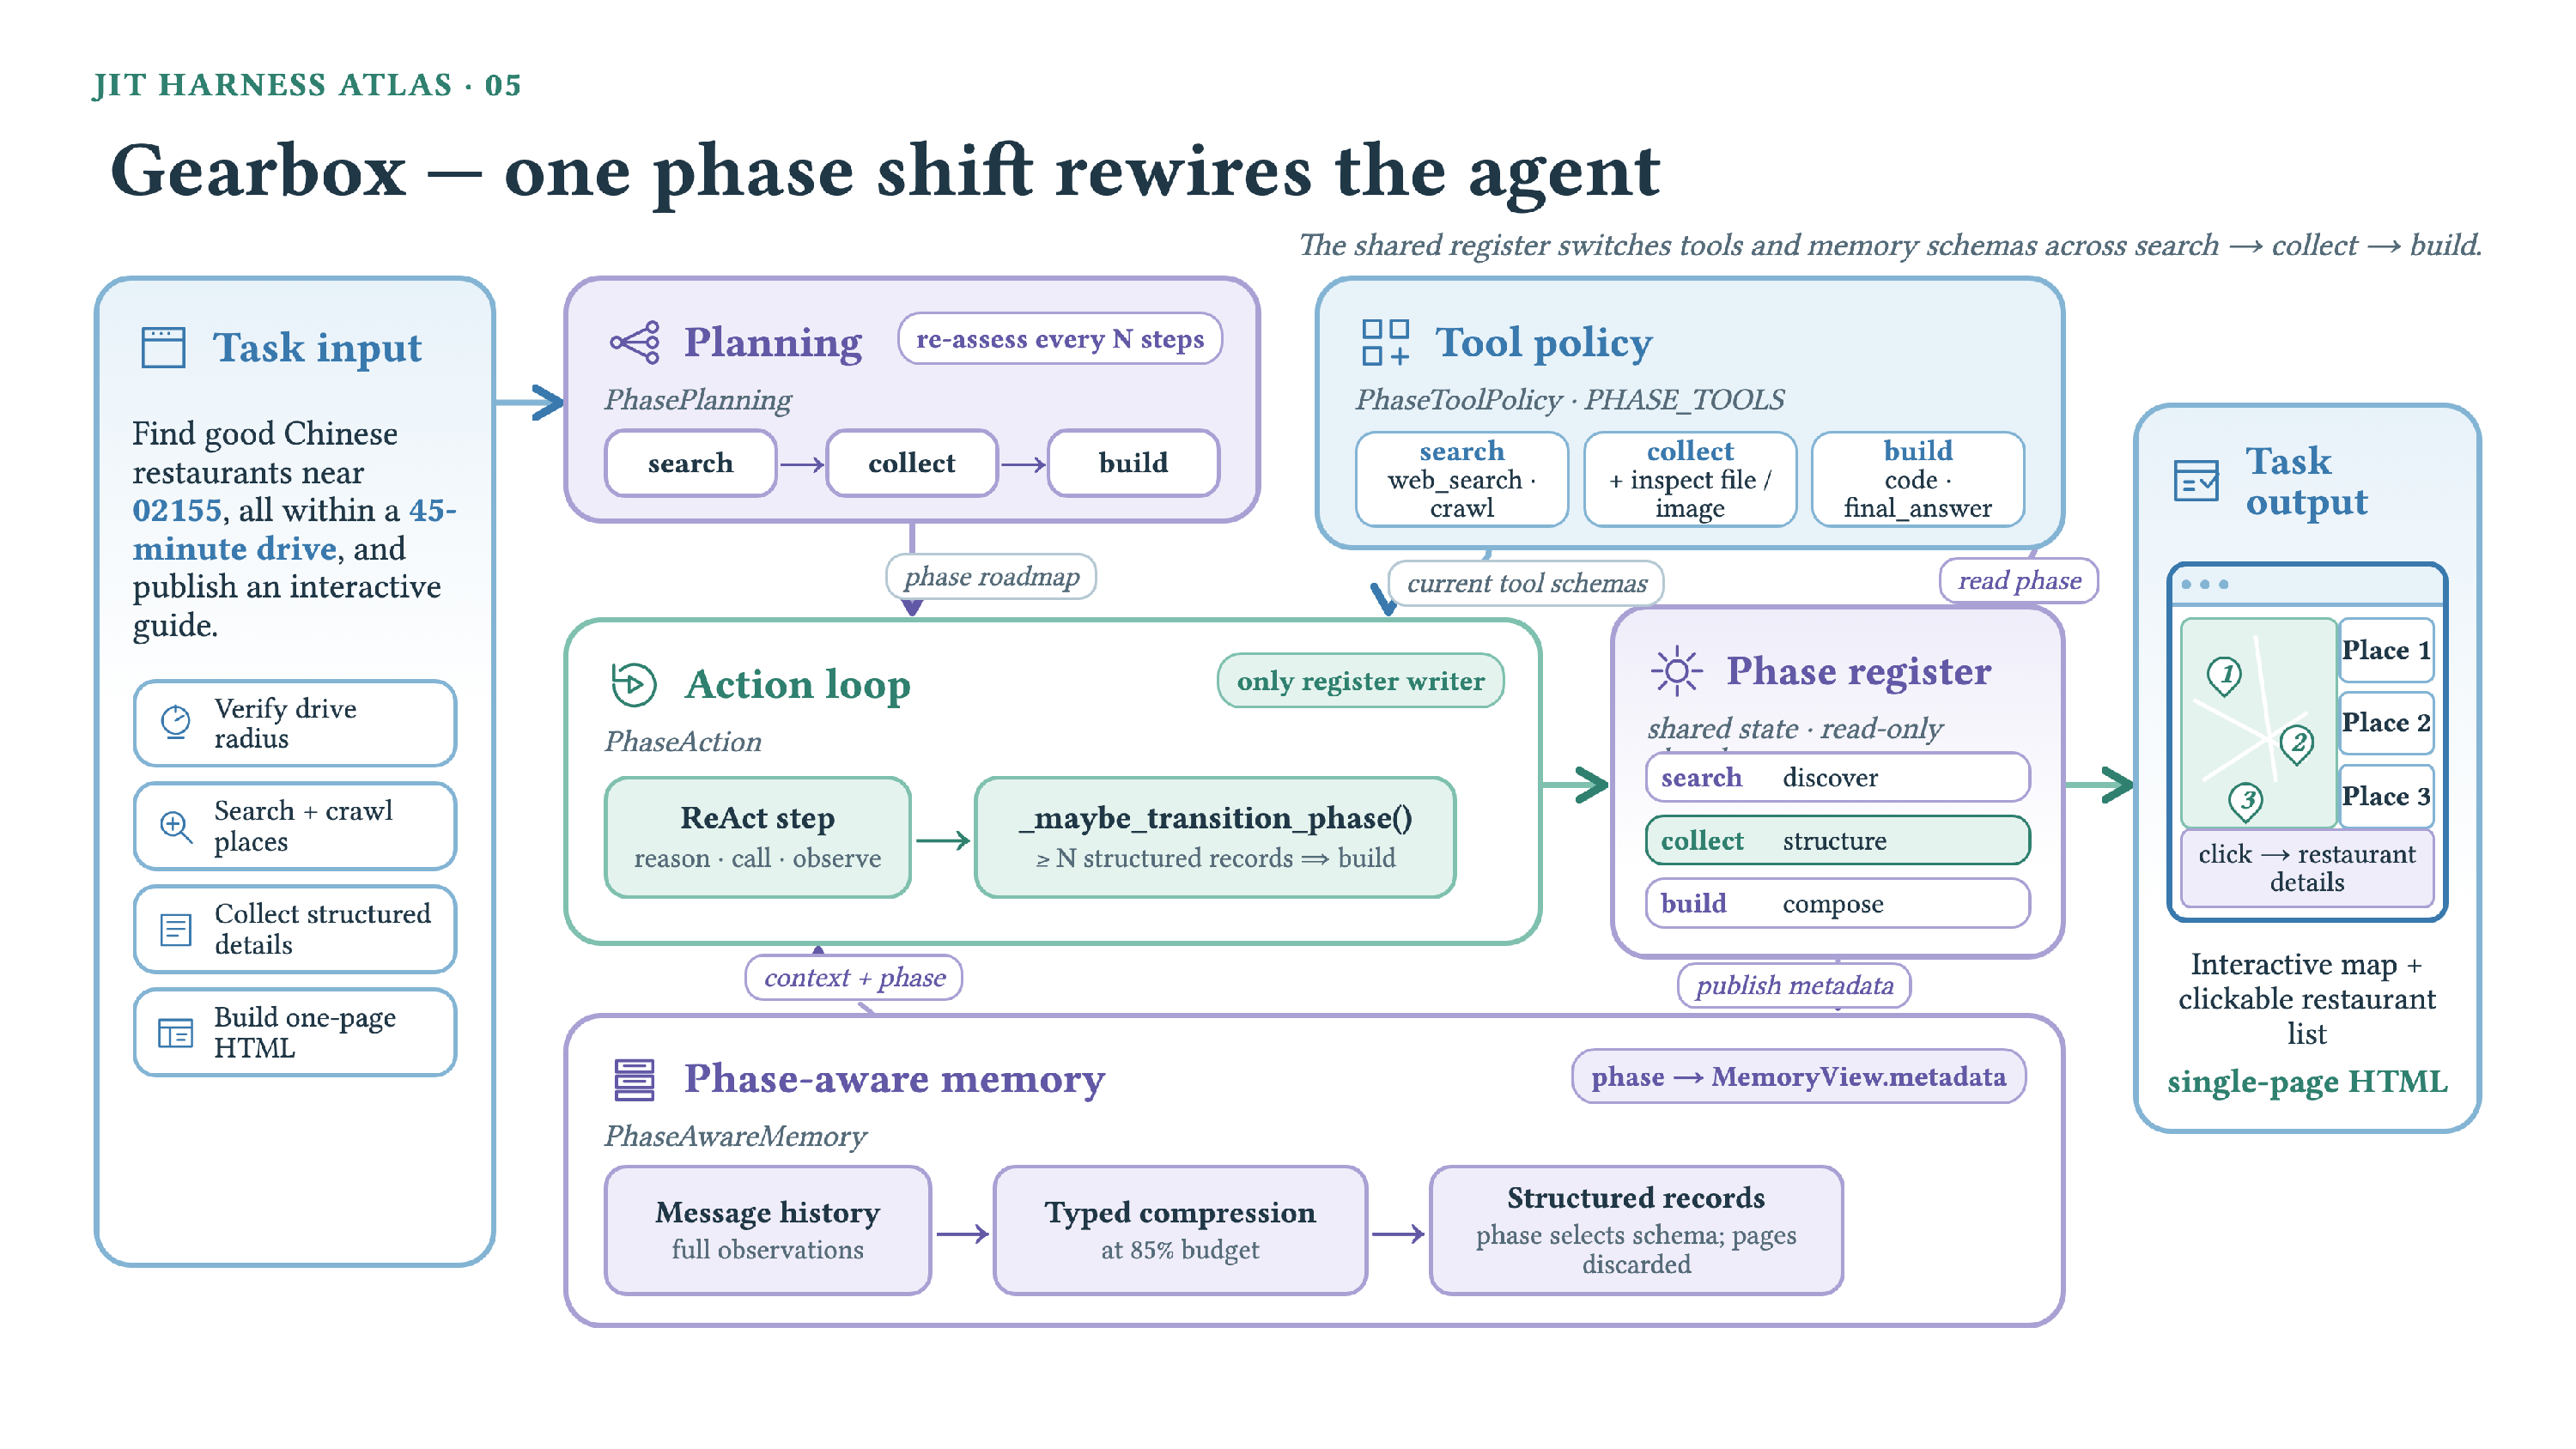
\includegraphics[width=\textwidth]{figures/harness_atlas_reworked/gearbox_flow.pdf}
    \vspace{-0.55em}
    \caption{\textbf{Gearbox：一次阶段转换即可重写智能体。}\texttt{PhaseAction} 是共享阶段寄存器的唯一写入者；\texttt{PhaseToolPolicy} 和 \texttt{PhaseAwareMemory} 读取该状态，同时切换所暴露的能力与有类型的记忆模式。}
    \label{fig:harness-gearbox}
\end{figure}
\begin{figure}[!htbp]
    \centering
    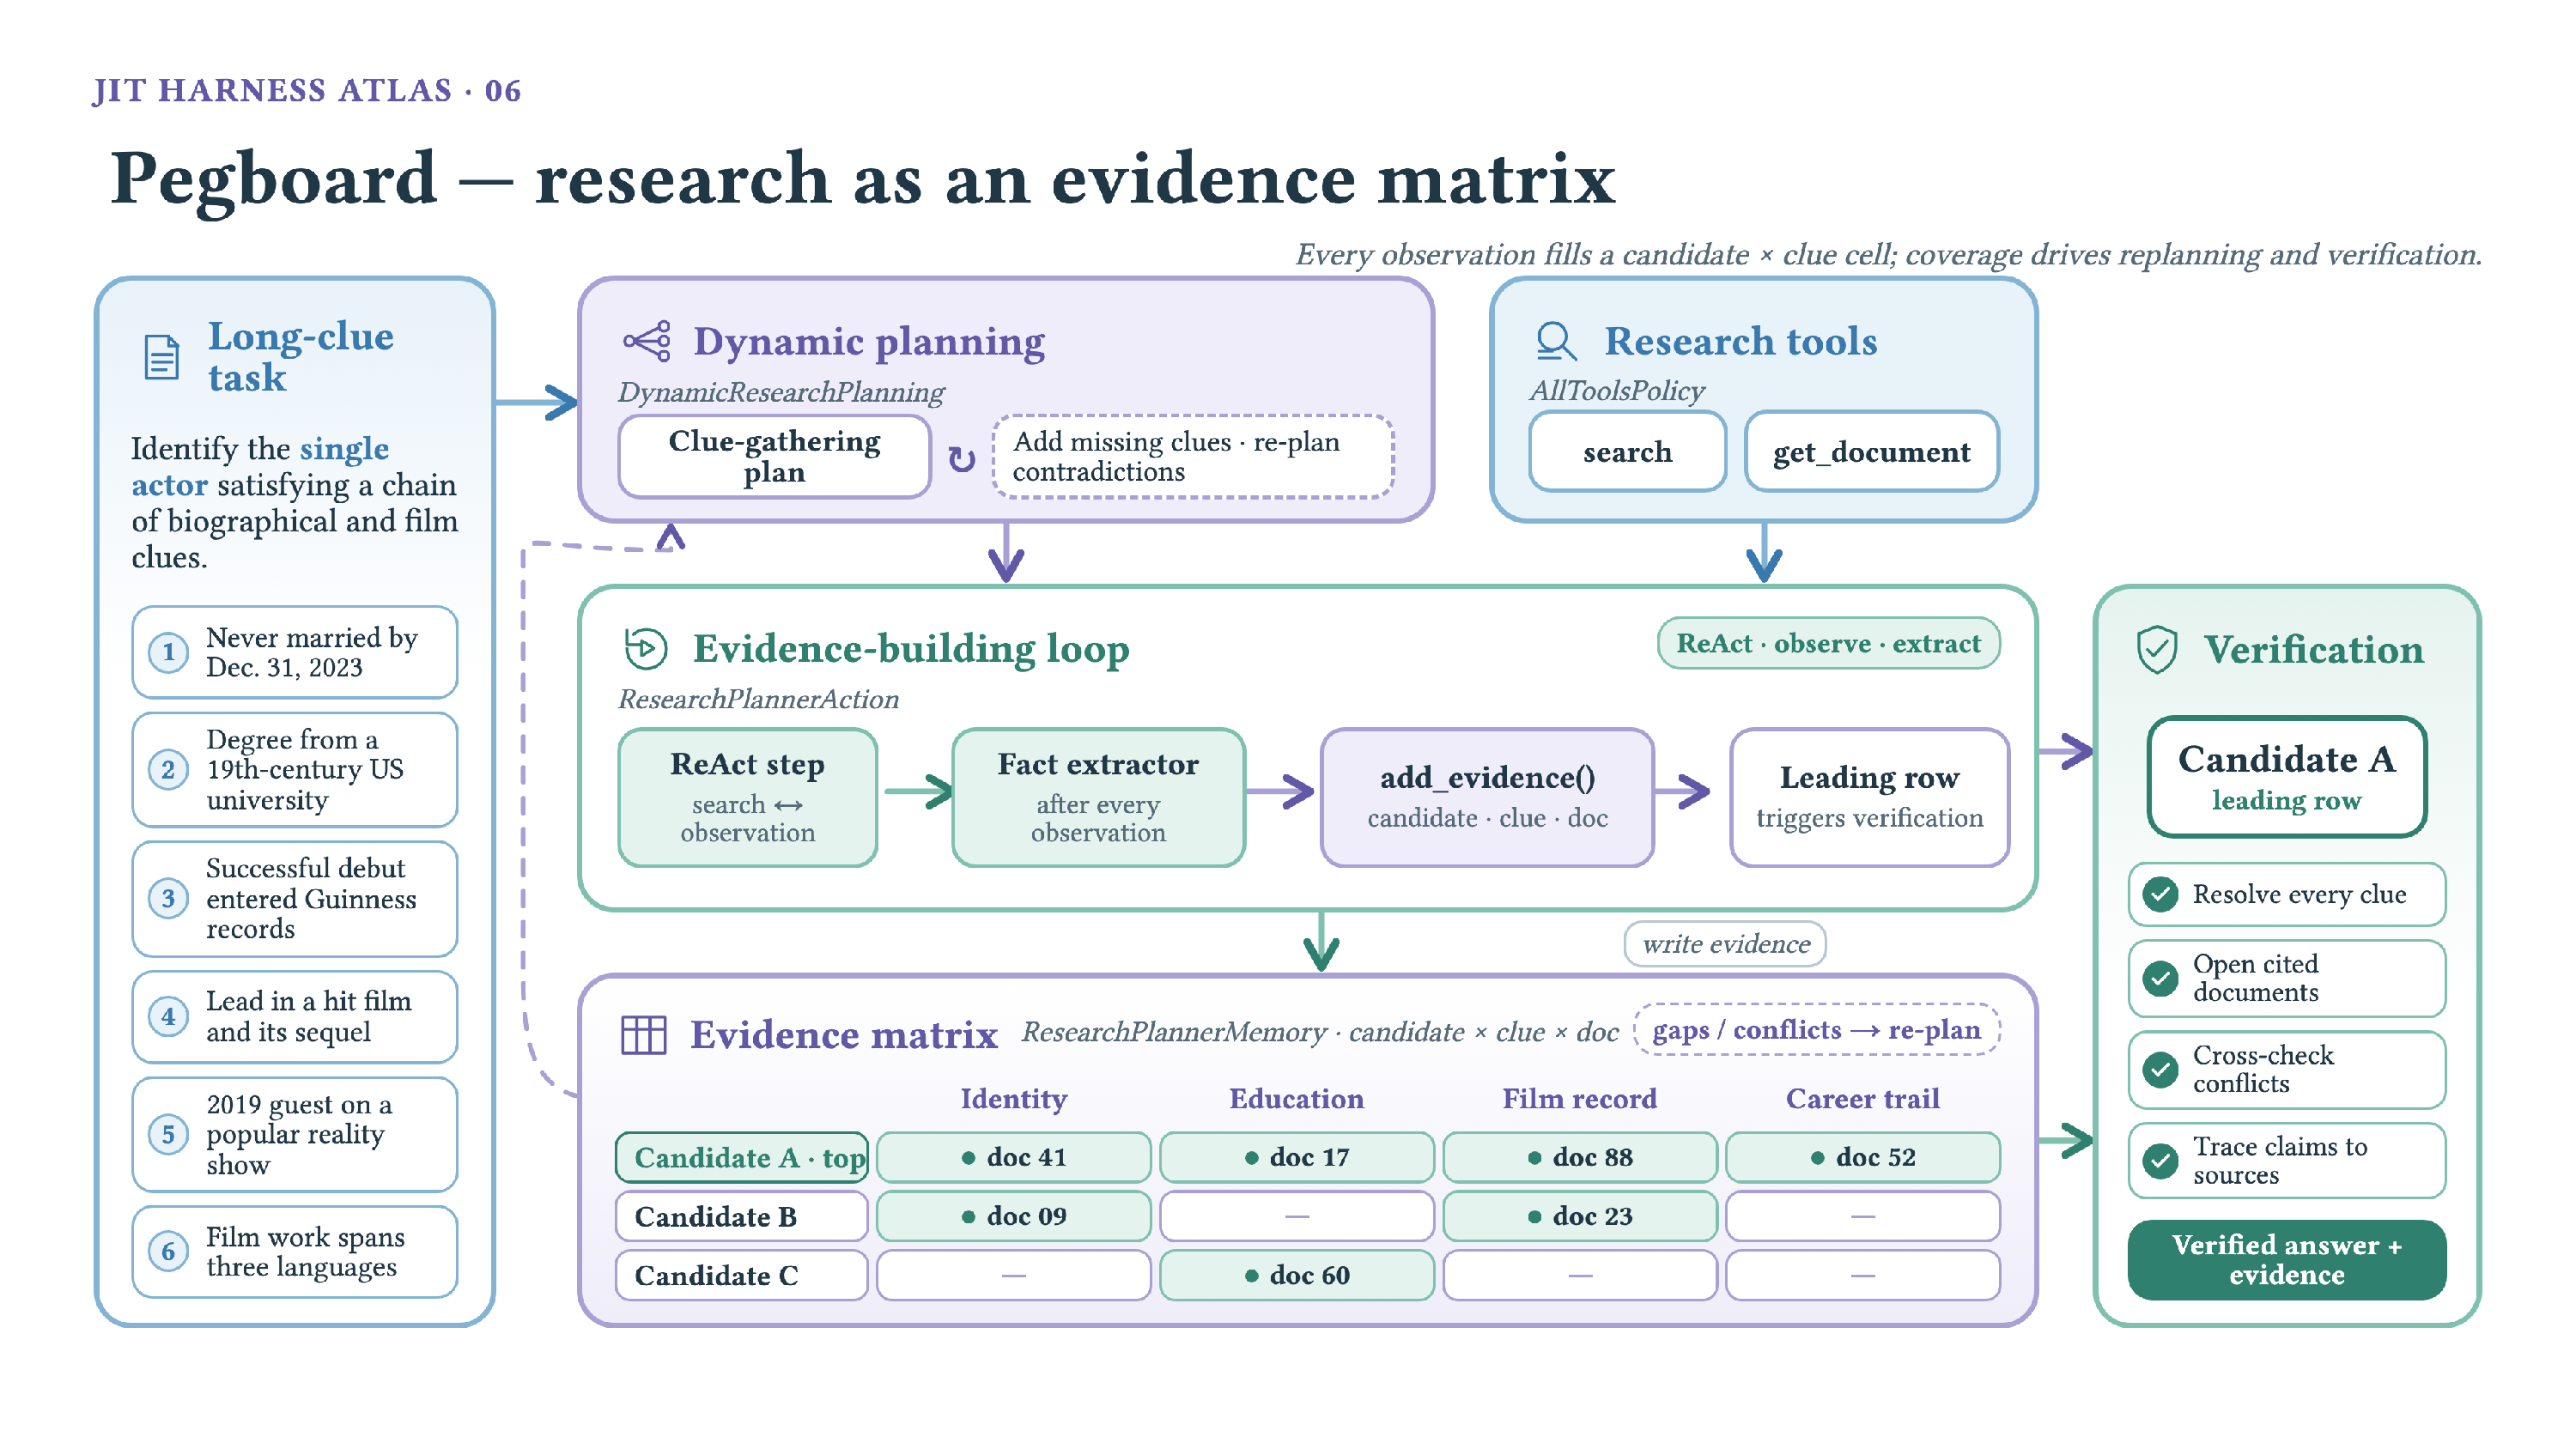
\includegraphics[width=\textwidth]{figures/harness_atlas_reworked/pegboard_flow.pdf}
    \vspace{-0.55em}
    \caption{\textbf{Pegboard：把研究表示为证据矩阵。}每个观察都被提取到带文档标识符的候选项 $\times$ 线索单元格中；矩阵覆盖度同时驱动 \texttt{DynamicResearchPlanning} 和向基于来源的验证阶段转换。}
    \label{fig:harness-pegboard}
\end{figure}

图~\ref{fig:harness-gearbox} 和图~\ref{fig:harness-pegboard} 展示了显式状态如何持续重塑后续决策。\textsc{Gearbox} 为如下任务生成：在指定驾驶半径内寻找中餐馆，并将结果发布为交互式单页指南。其 \texttt{PhaseAction} 是共享\textit{搜索--收集--构建}寄存器的唯一写入者；只有收集到足够多结构化餐馆记录后，系统才会转入构建阶段。\texttt{PhaseToolPolicy} 与 \texttt{PhaseAwareMemory} 都读取该寄存器，从 Web 发现切换到记录检查，再切换到编码与发布，同时把观察压缩为当前阶段所需的模式。由于任务形态从证据获取转为工件构建，模型由此创建了一台阶段机。

\textsc{Pegboard} 则处理一个由六条人物传记与电影线索定义的身份识别问题。它把进度表示为候选项 $\times$ 线索矩阵，其中每条提取的主张都保留其文档标识符。空单元格和矛盾推动 \texttt{DynamicResearchPlanning} 开展定向搜索；当某一行获得足够支持时，则触发独立验证阶段，重新打开被引用的文档并解决冲突。不同于一般研究记录，这种状态让覆盖度与来源溯源直接转化为可执行信号。与 \textsc{Gearbox} 的对比表明，生成状态既可以是小型阶段变量，也可以是按任务塑形的证据结构，取决于需要用什么来支配下一动作。

\begin{figure}[!htbp]
    \centering
    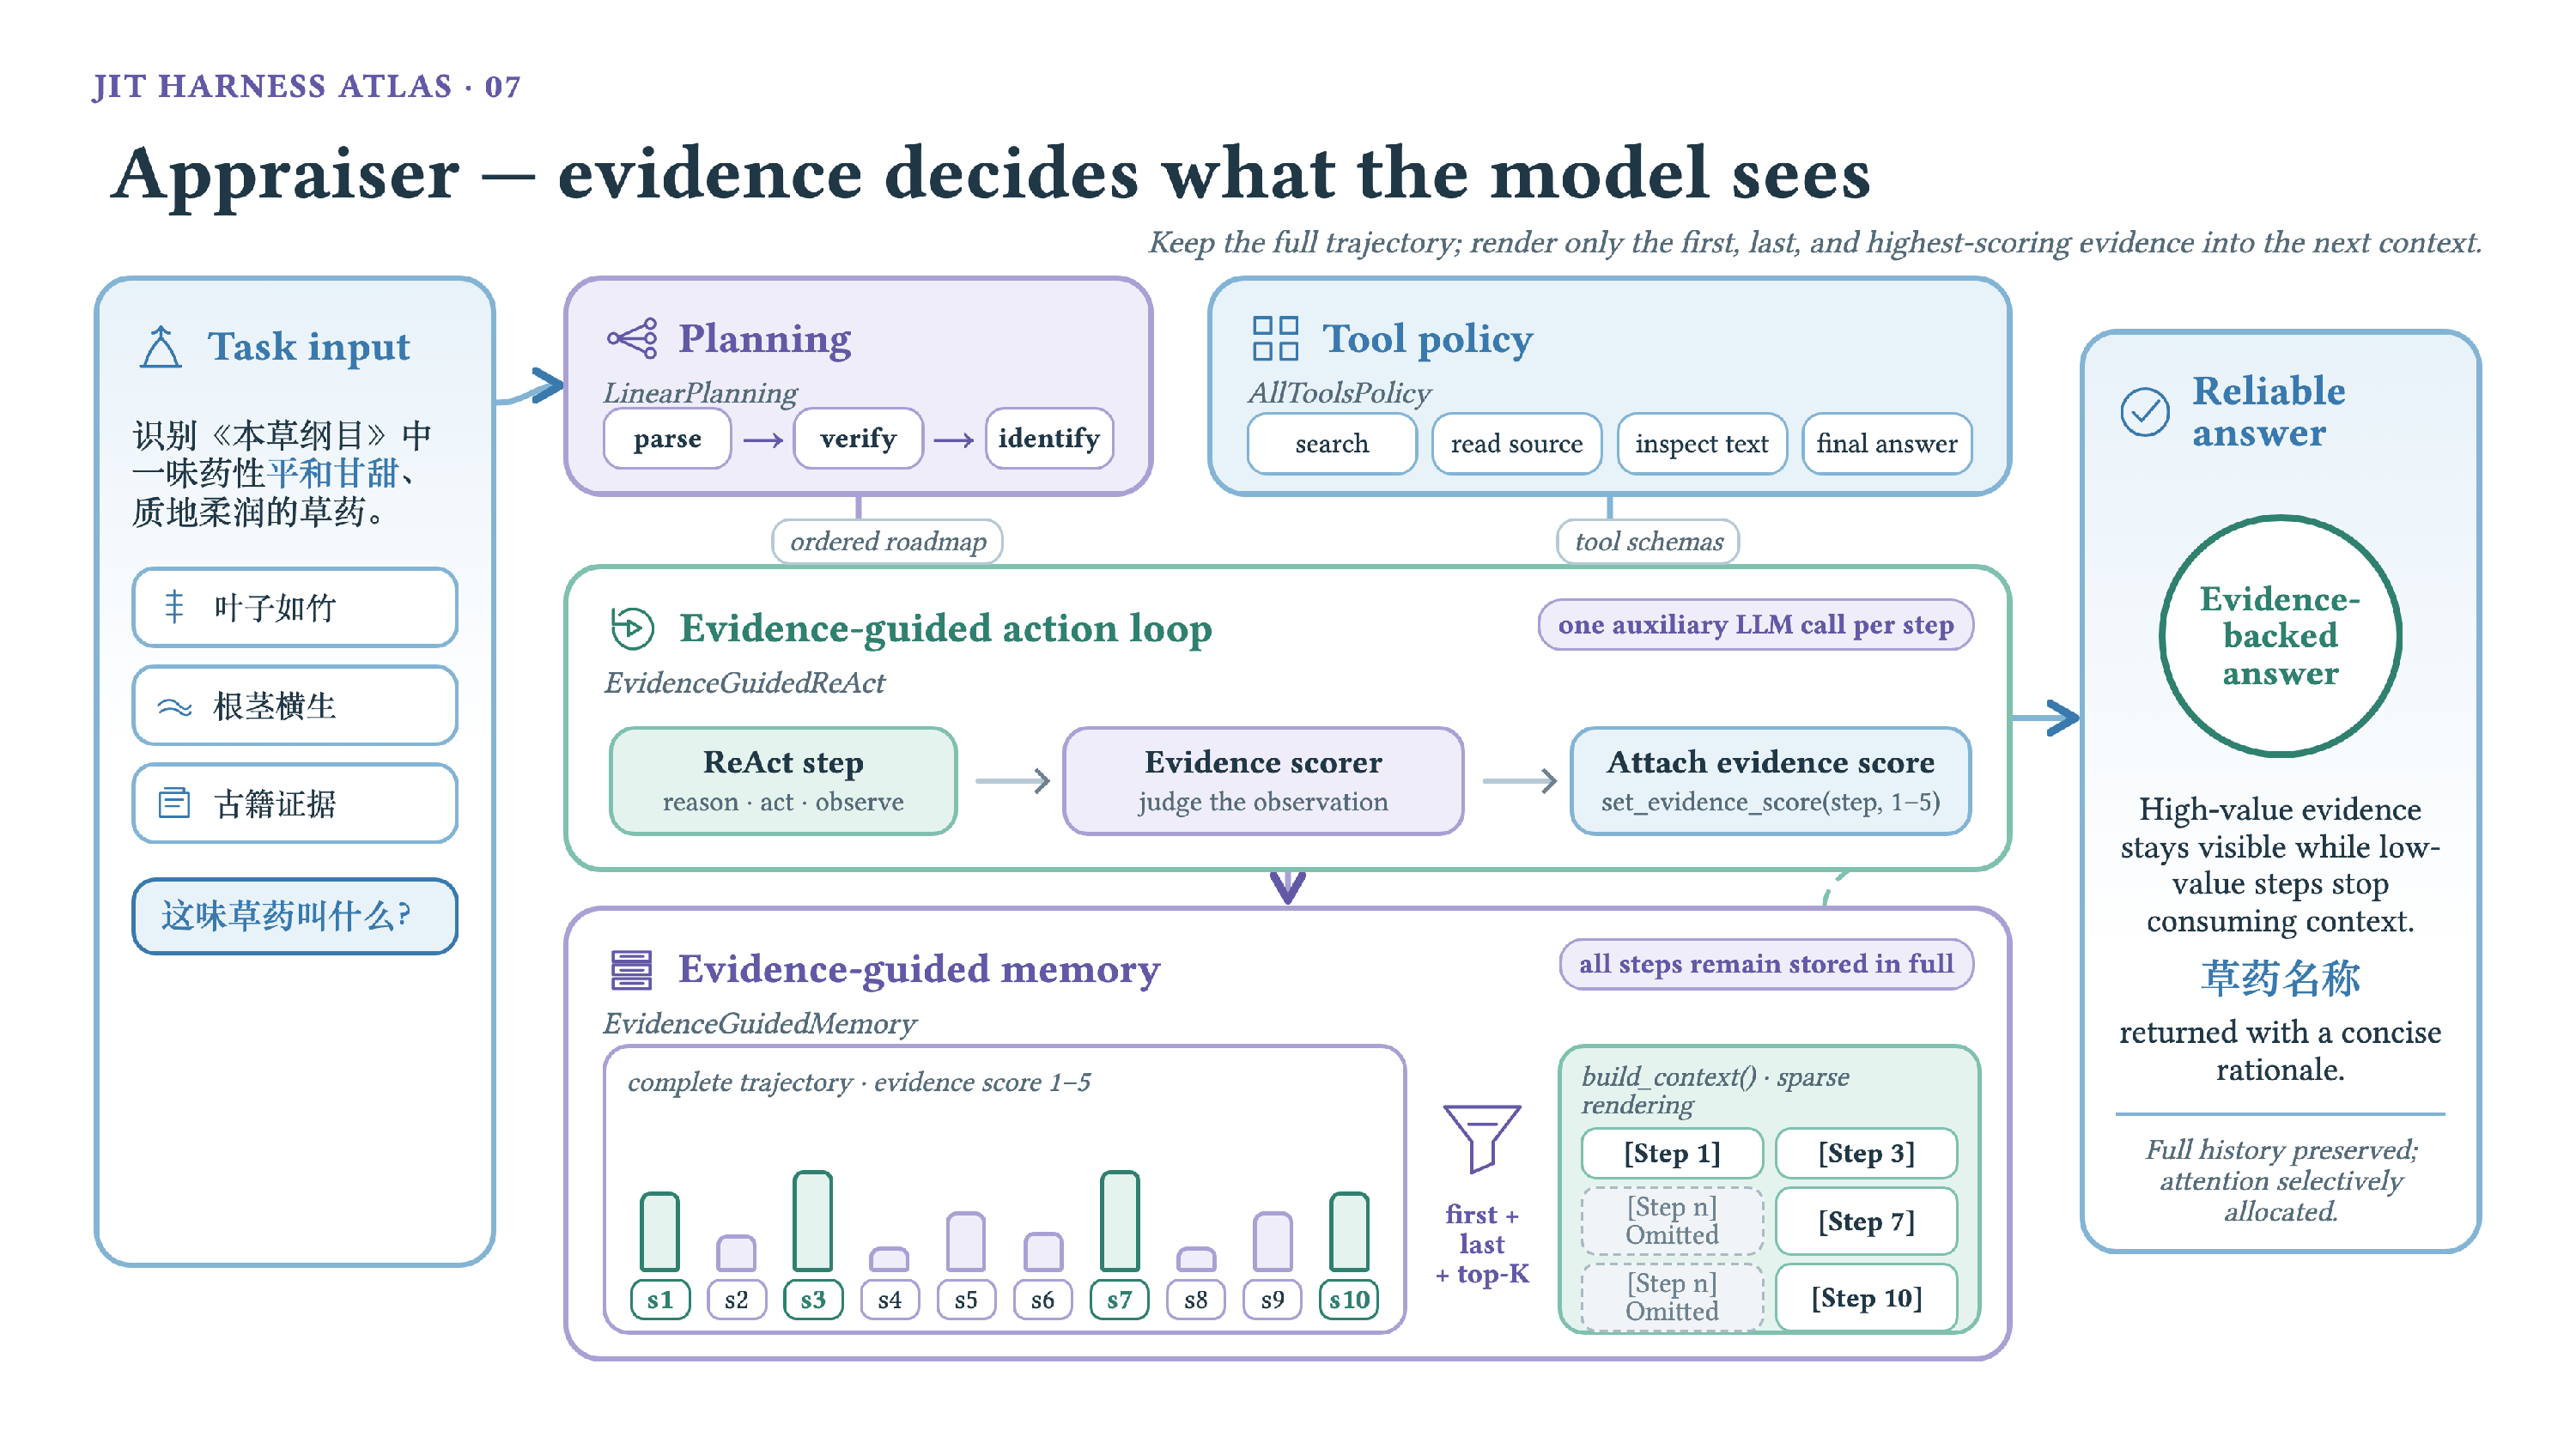
\includegraphics[width=\textwidth]{figures/harness_atlas_reworked/appraiser_flow.pdf}
    \vspace{-0.55em}
    \caption{\textbf{Appraiser：证据决定模型看到什么。}\texttt{EvidenceGuidedReAct} 为每一步评分；\texttt{EvidenceGuidedMemory} 存储完整运行过程，但只把最初、最后和得分最高的 $K$ 个观察渲染进 \texttt{build\_context()}。}
    \label{fig:harness-appraiser}
\end{figure}
\begin{figure}[!htbp]
    \centering
    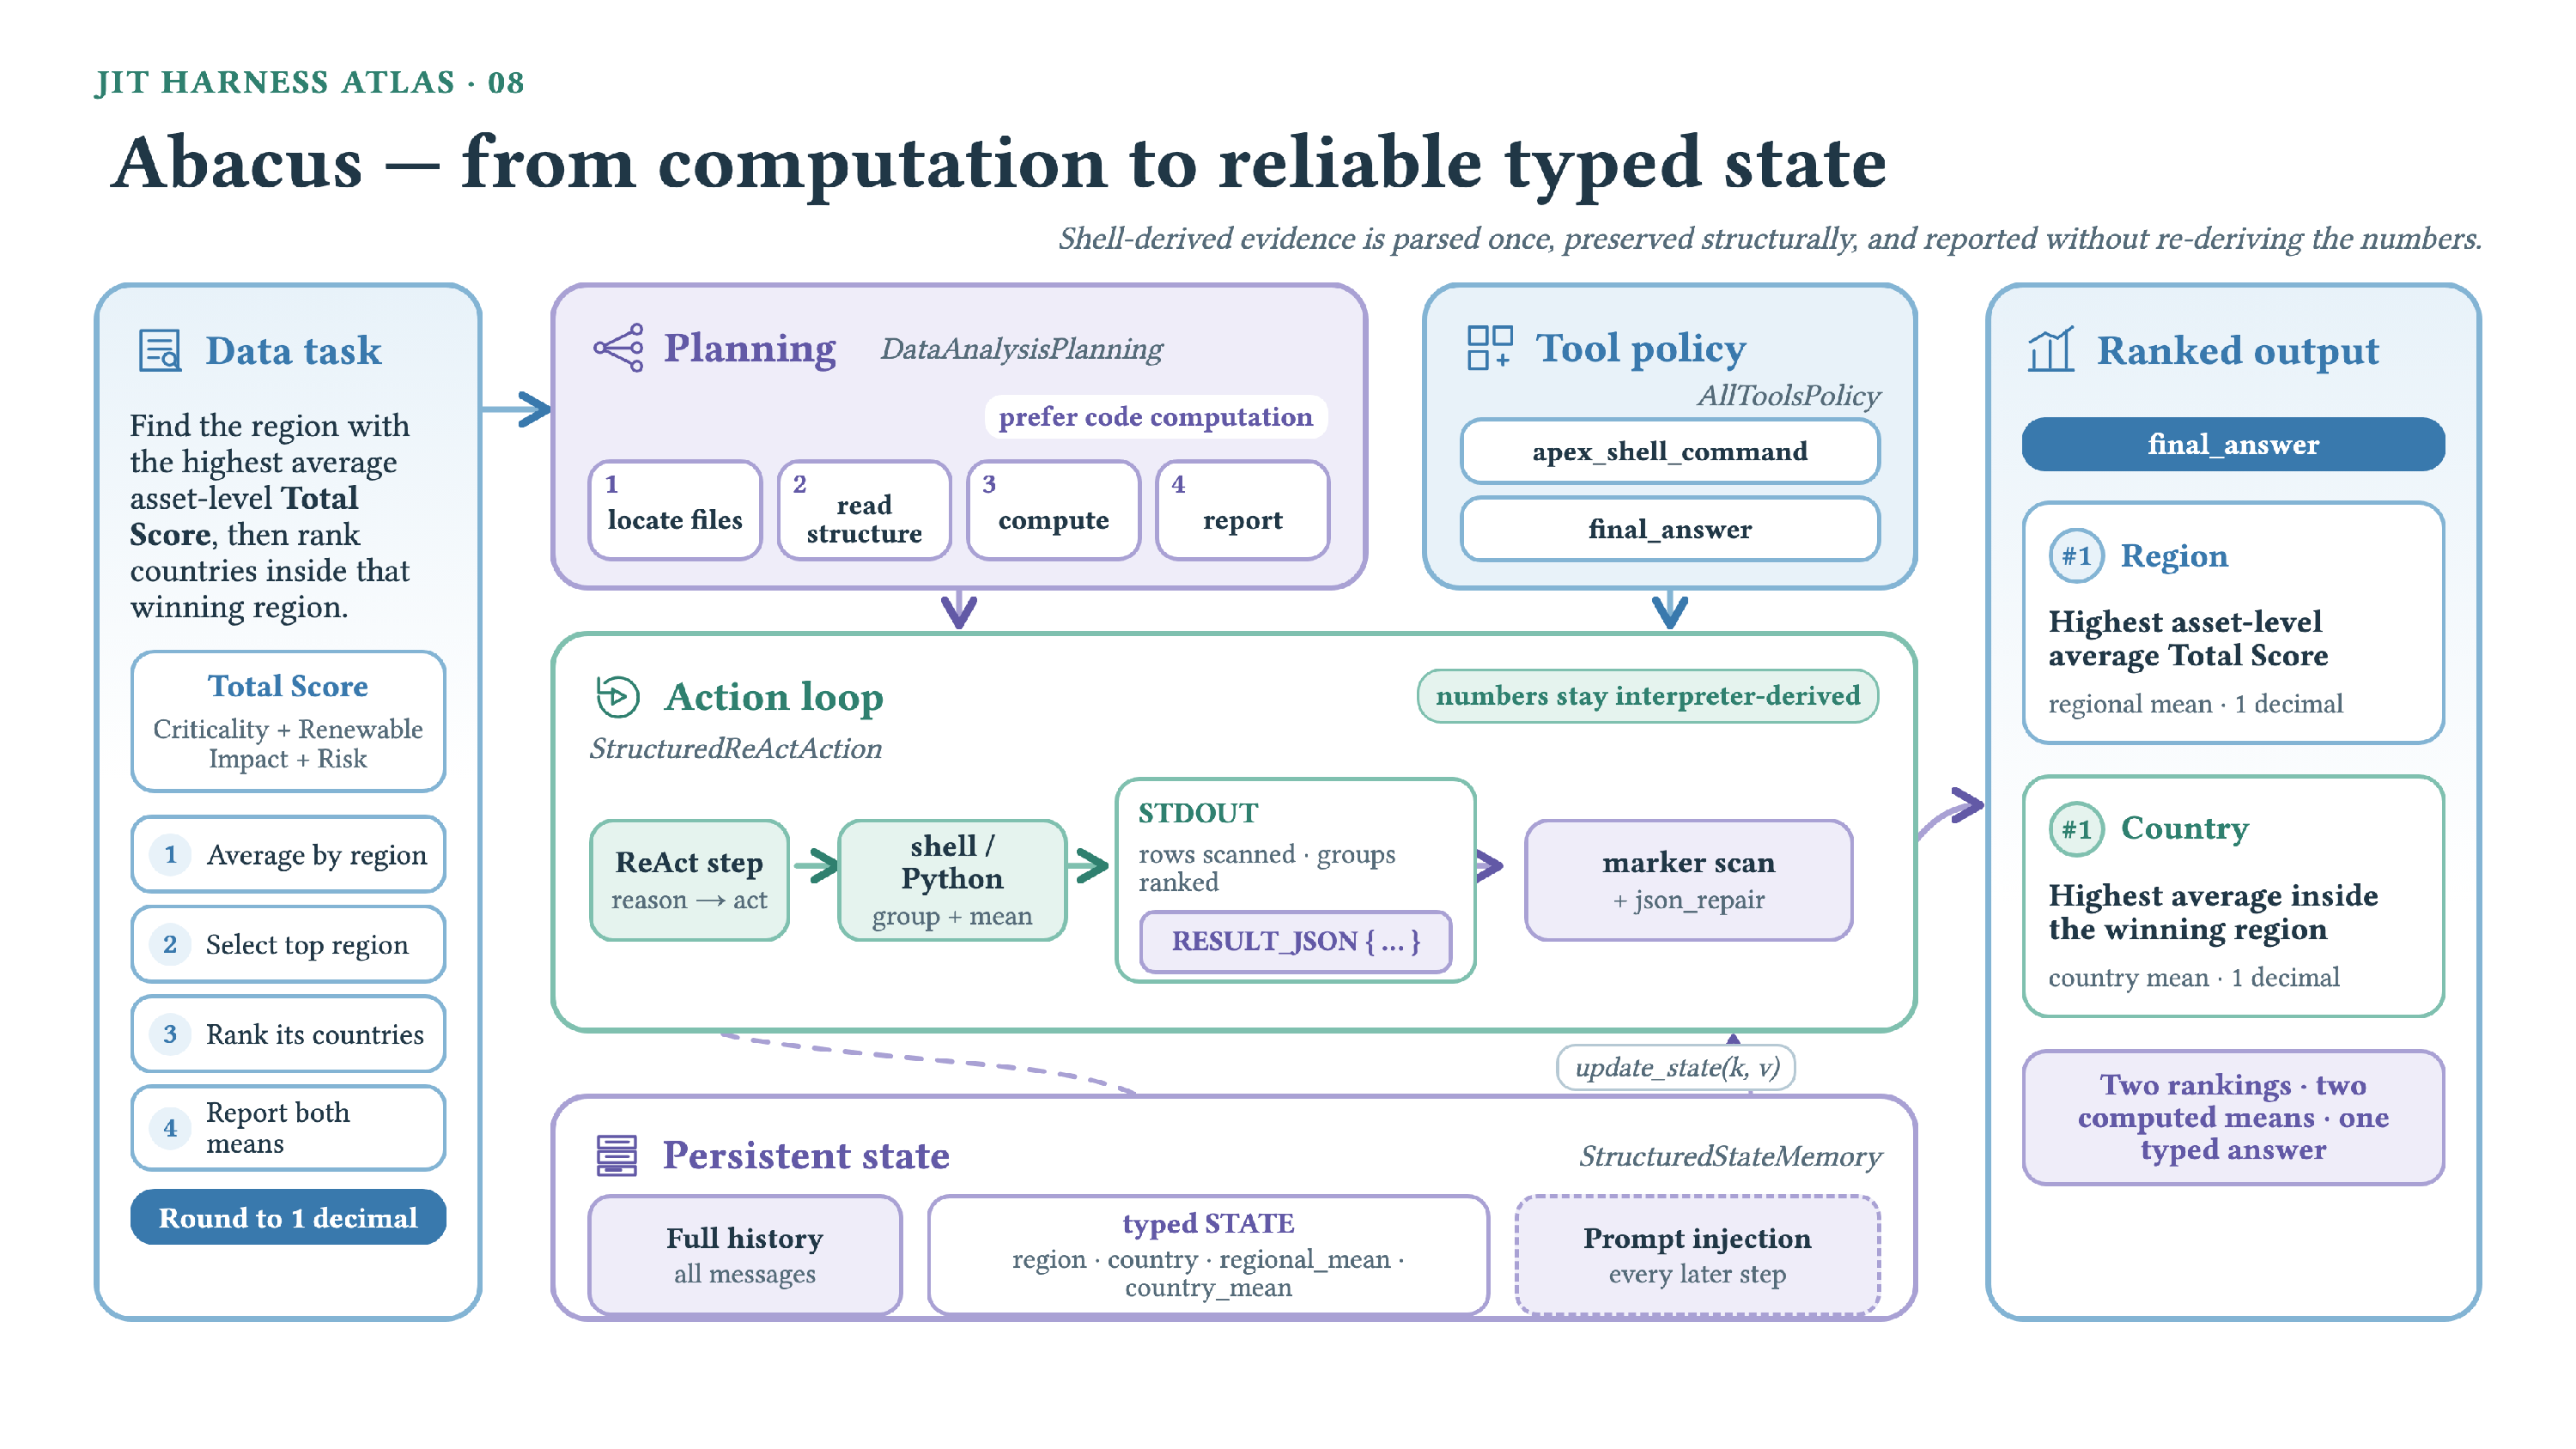
\includegraphics[width=\textwidth]{figures/harness_atlas_reworked/abacus_flow.pdf}
    \vspace{-0.55em}
    \caption{\textbf{Abacus：从计算走向可靠的有类型状态。}\texttt{StructuredReActAction} 执行 shell 或 Python 代码，从标准输出中提取 \texttt{RESULT\_JSON} 载荷，并更新 \texttt{StructuredStateMemory}，无需模型重新推导计算值。}
    \label{fig:harness-abacus}
\end{figure}

图~\ref{fig:harness-appraiser} 和图~\ref{fig:harness-abacus} 定制后续推理从既往执行中接收的内容。\textsc{Appraiser} 通过协调植物学特征与文本证据，回答一个经典本草身份识别问题。每次搜索或阅读后，辅助评分器都会为观察赋予证据价值；\texttt{EvidenceGuidedMemory} 为可审计性保留完整轨迹，但只把最初、最后和得分最高的 $K$ 个观察渲染到下一上下文。由此，低价值探索不再与最有助于识别的段落争夺上下文，同时没有证据从持久历史中被抹除。该支架专门适配这样一种检索任务：其主要瓶颈是证据显著性，而非工具选择。

\textsc{Abacus} 面向一项数值分析请求生成：先比较各地区平均值，再对胜出地区内的国家排序。该支架有意将聚合移出语言模型推理：\texttt{StructuredReActAction} 调用 shell 或 Python，从标准输出中提取带标记的 \texttt{RESULT\_JSON} 载荷，必要时修复其语法，并把数值写入 \texttt{StructuredStateMemory}。随后，地区、国家、地区均值和国家均值会作为有类型状态注入每个后续步骤，使最终答案报告解释器计算得到的量，而非从文字中重新推导。两个案例都保留完整审计轨迹，但都围绕自身任务占主导的可靠性要求渲染工作视图：一个重证据选择，另一个重数值保真。

\begin{figure}[!htbp]
    \centering
    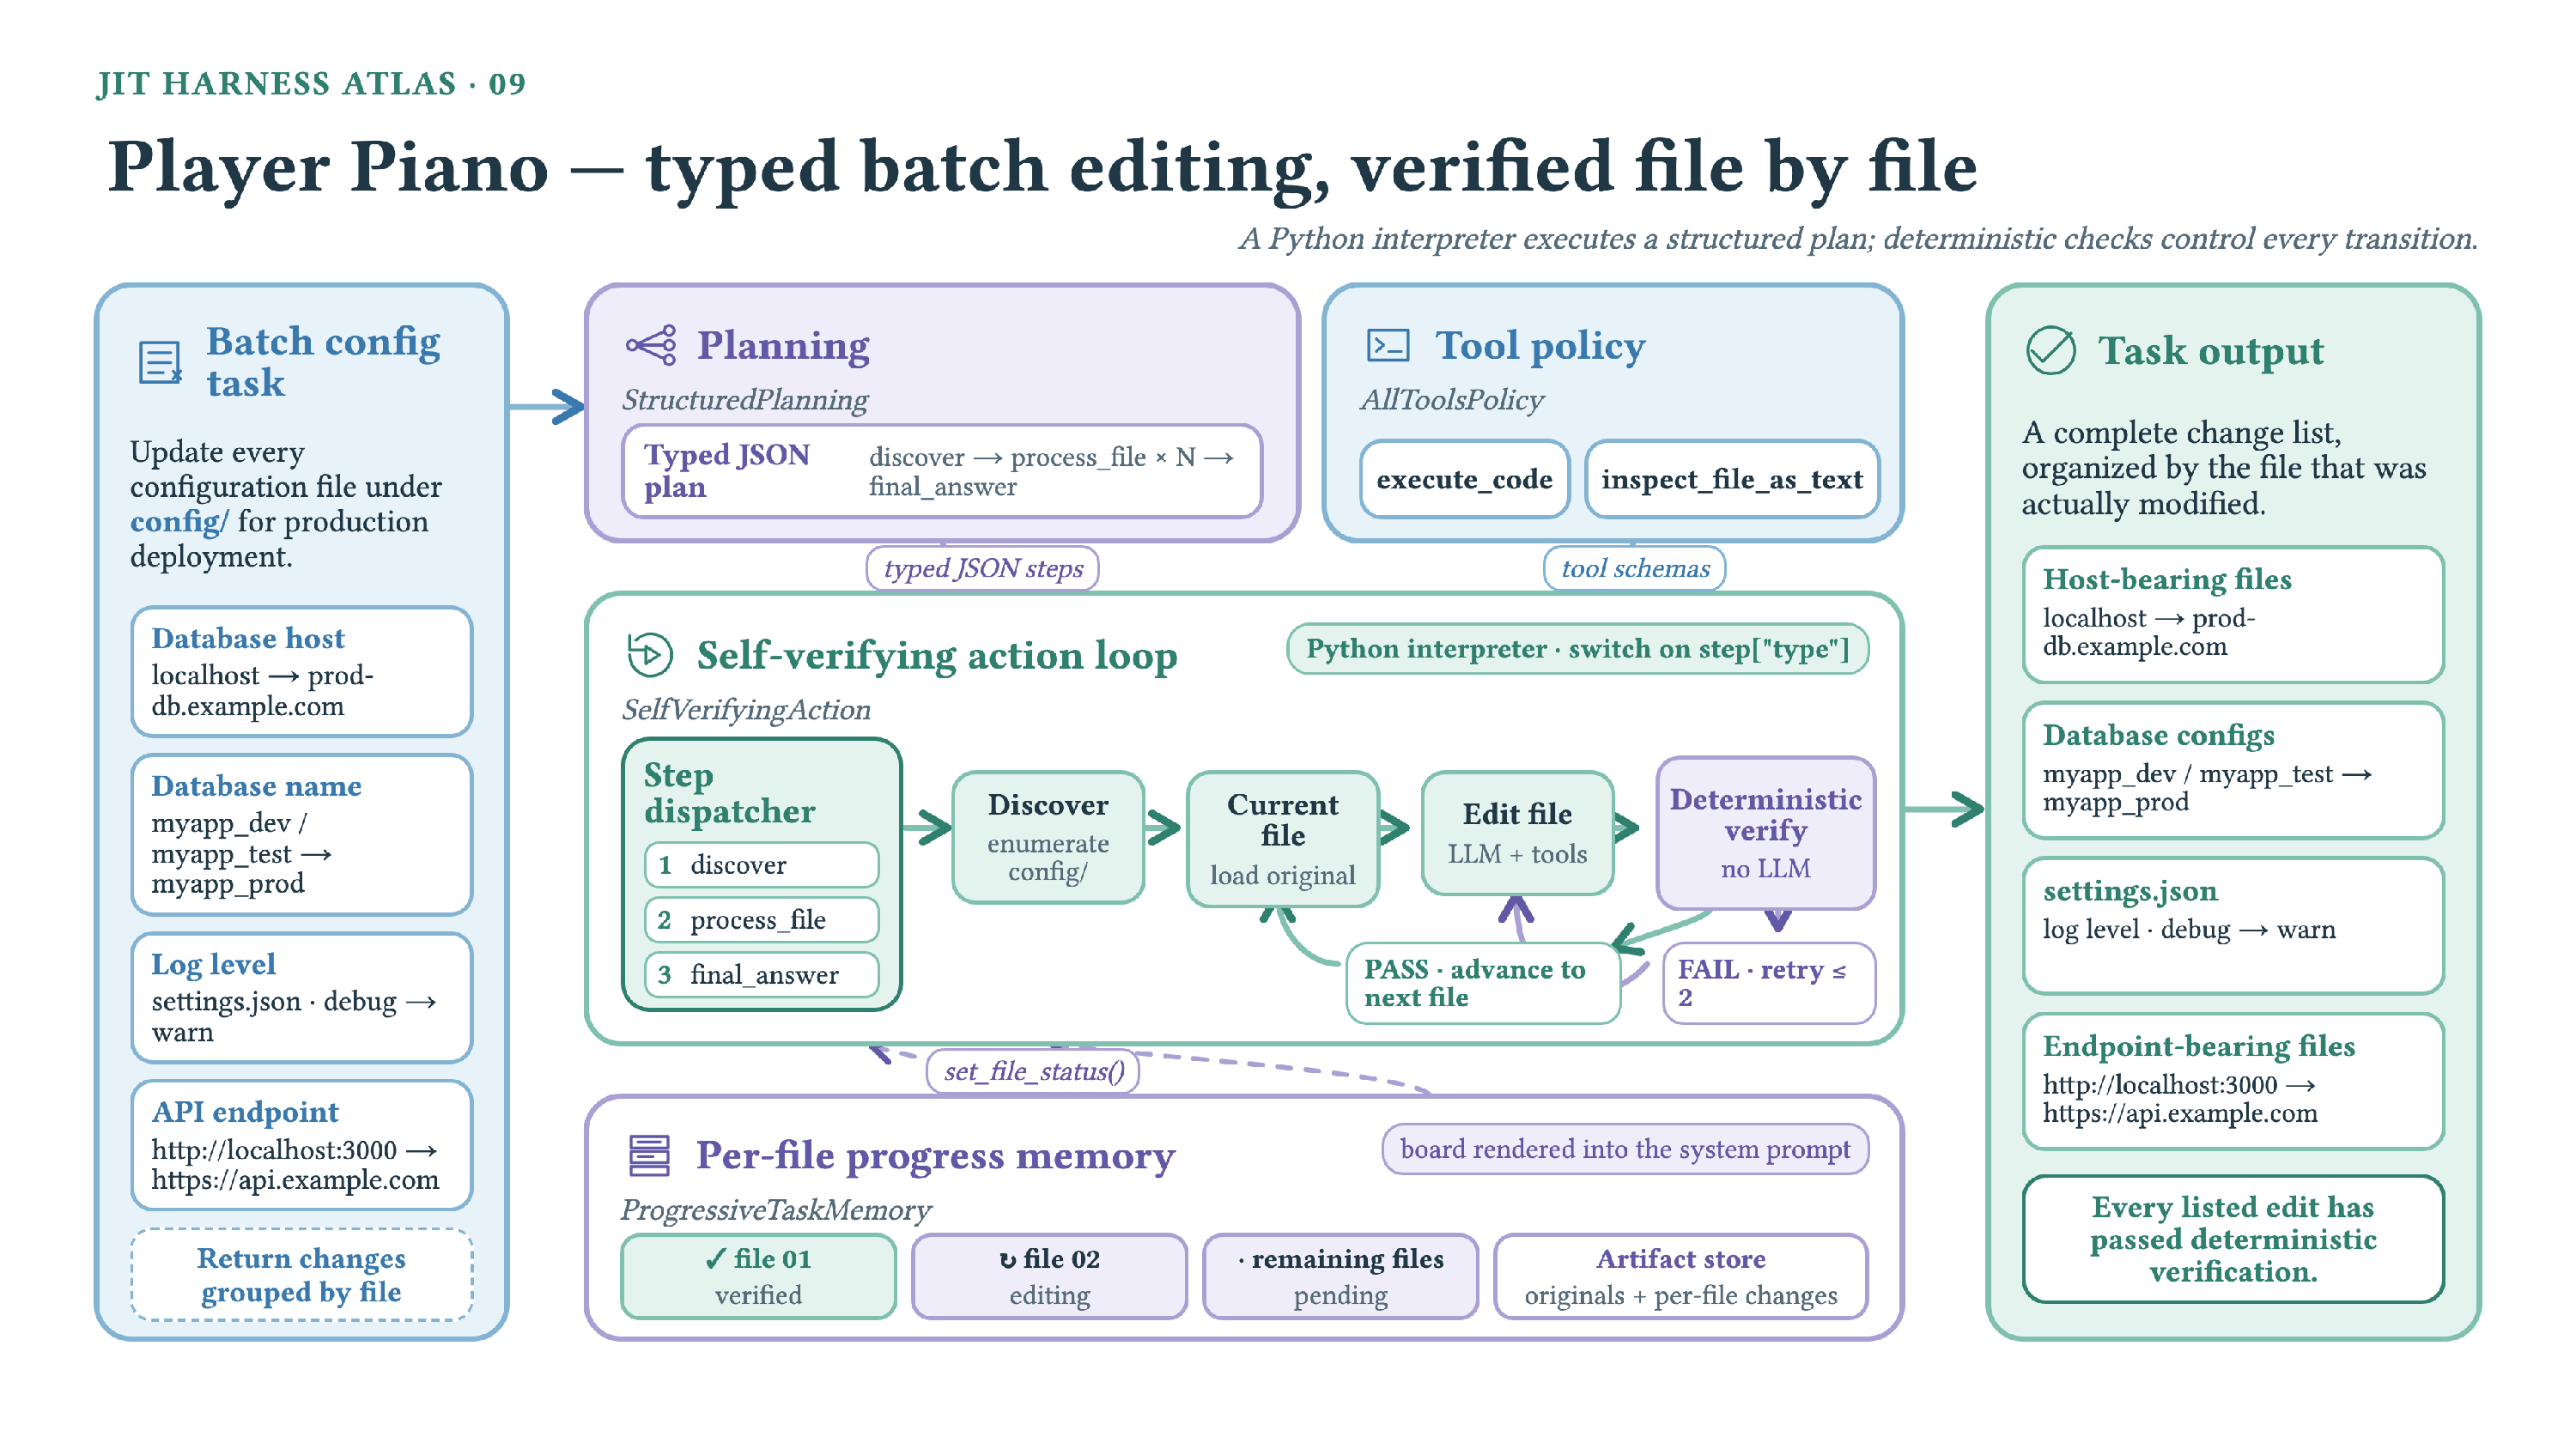
\includegraphics[width=\textwidth]{figures/harness_atlas_reworked/player_piano_flow.pdf}
    \vspace{-0.9em}
    \caption{\textbf{Player Piano：有类型的批量编辑，逐文件验证。}Python 调度器解释 \texttt{StructuredPlanning} 步骤，\texttt{SelfVerifyingAction} 无需大语言模型即可检查每次编辑，而 \texttt{ProgressiveTaskMemory} 维护逐文件看板和工件存储。}
    \label{fig:harness-player-piano}
\end{figure}
\begin{figure}[!htbp]
    \centering
    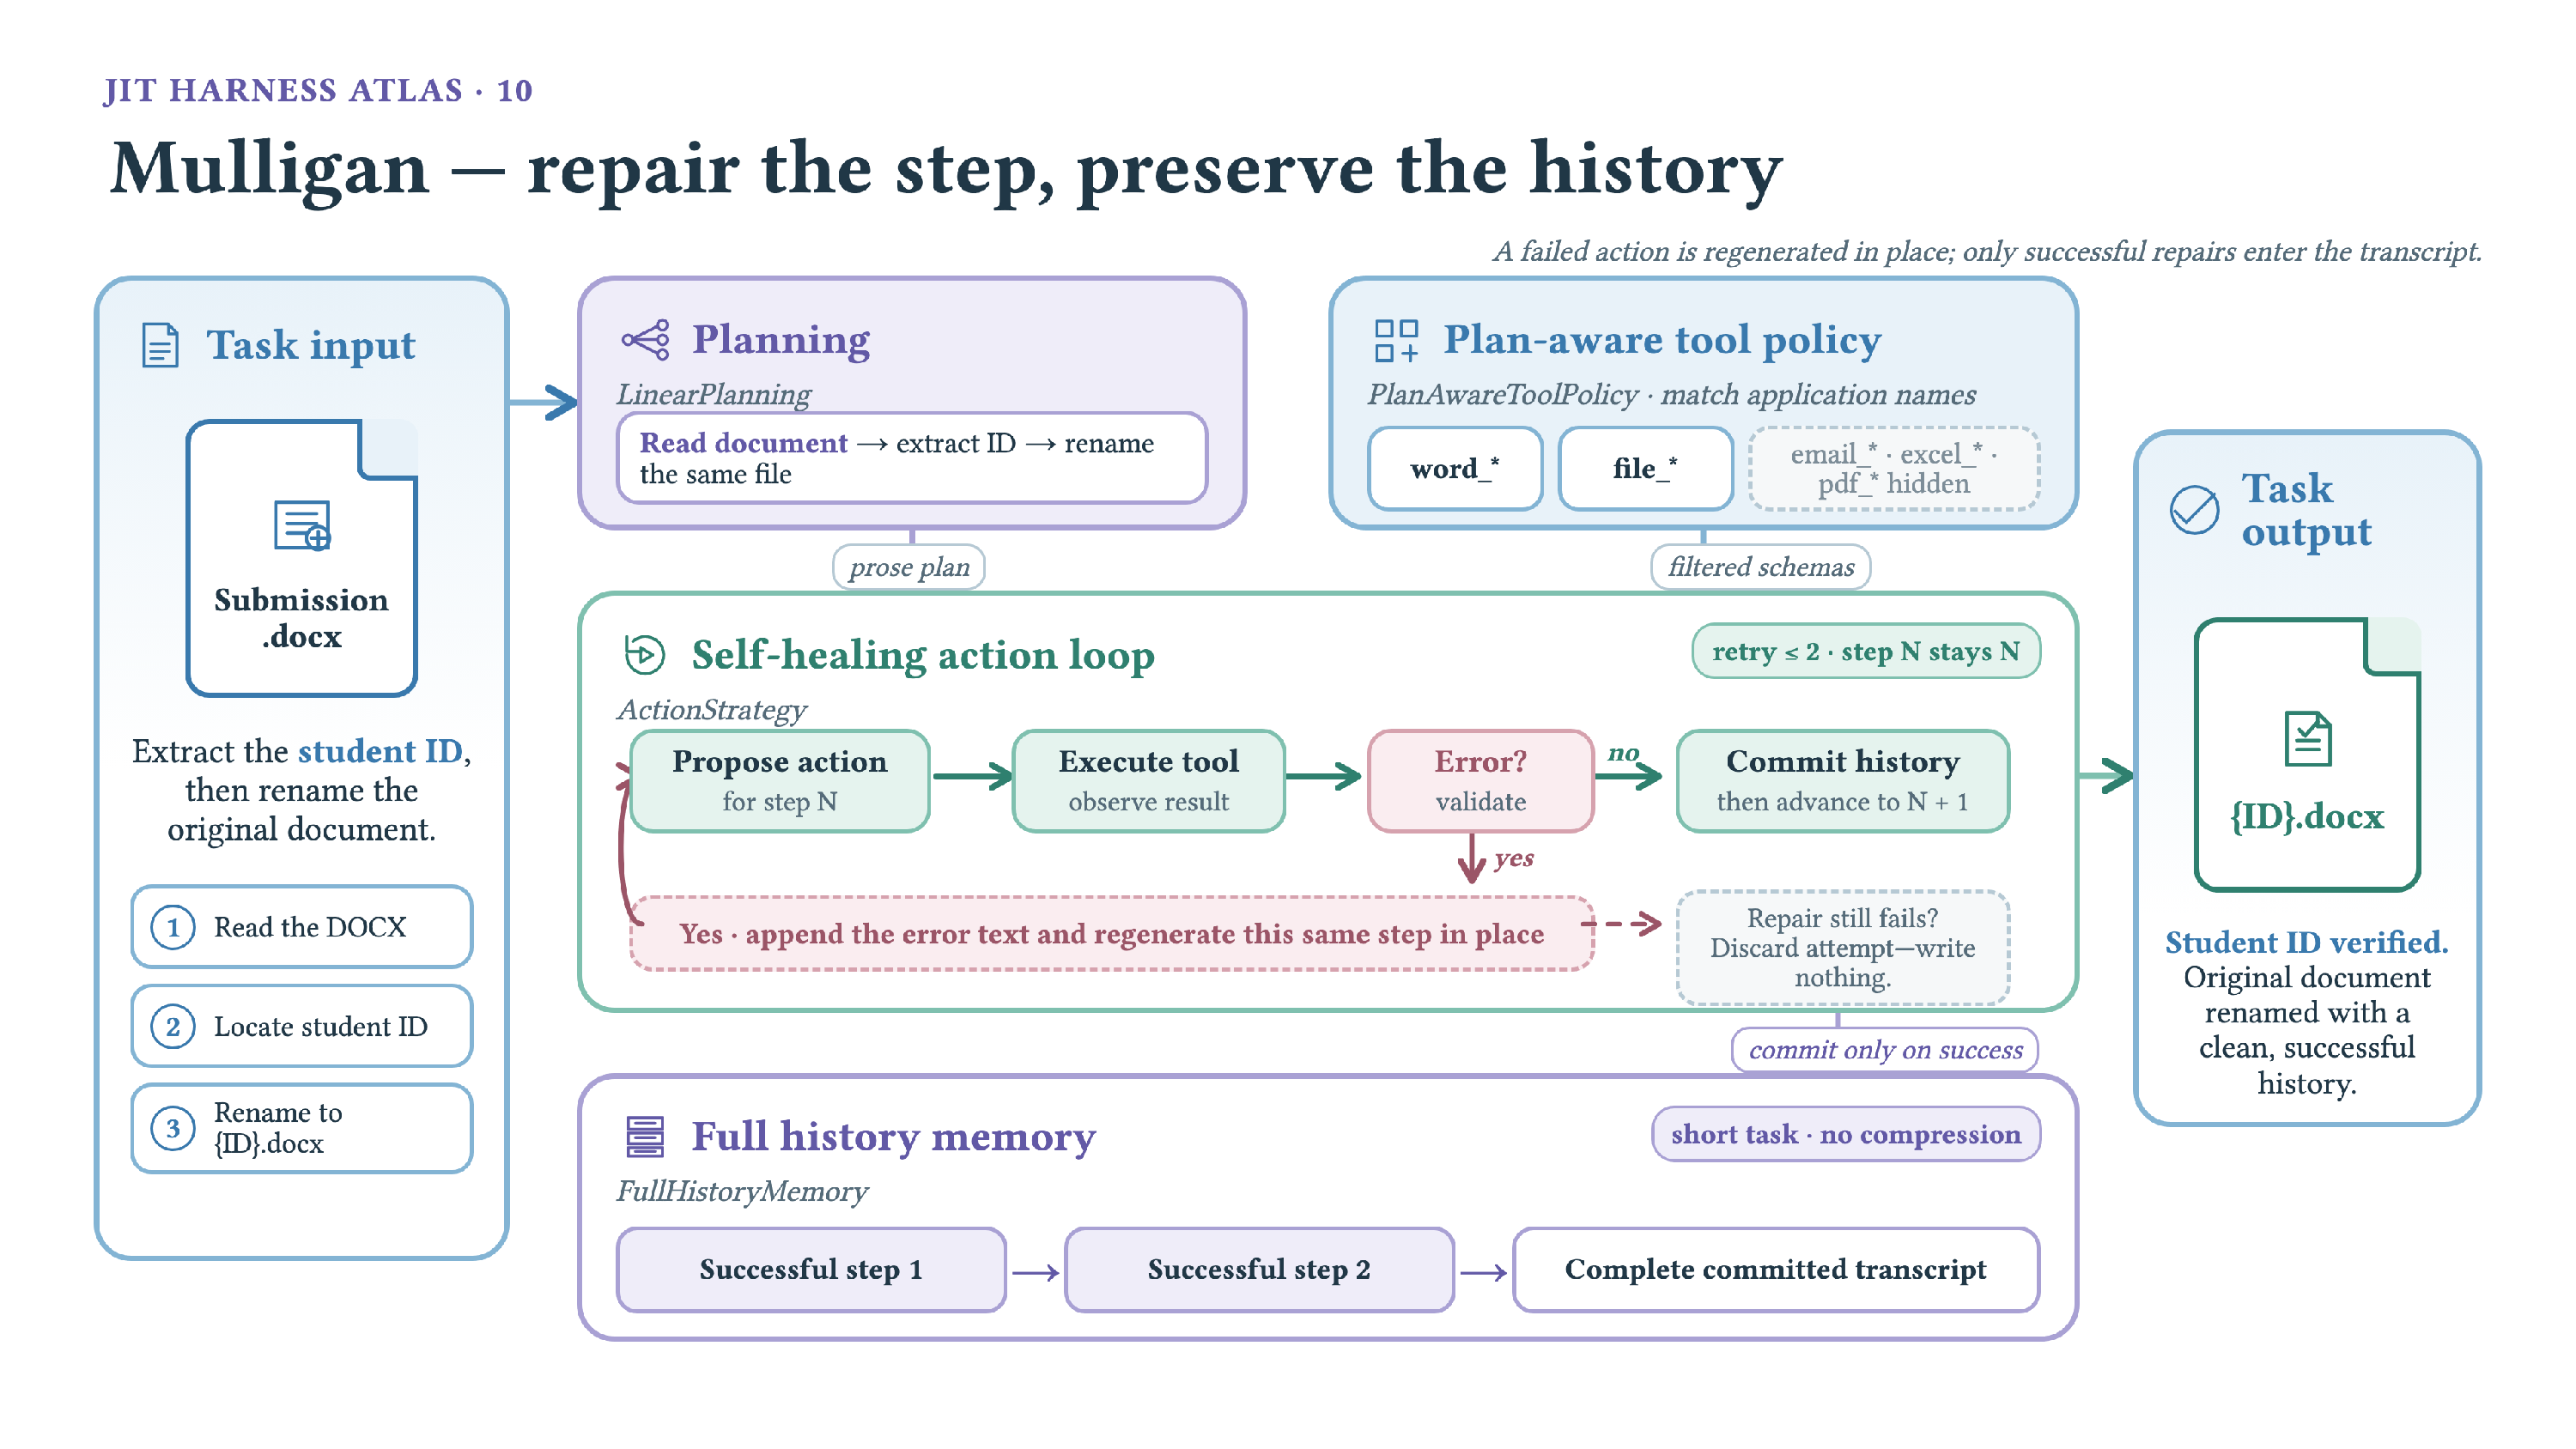
\includegraphics[width=\textwidth]{figures/harness_atlas_reworked/mulligan_flow.pdf}
    \vspace{-0.9em}
    \caption{\textbf{Mulligan：修复步骤，保留历史。}\texttt{PlanAwareToolPolicy} 只暴露与计划相关的文件和文档工具；失败动作在同一步骤重新生成，而 \texttt{FullHistoryMemory} 只接收成功执行。}
    \label{fig:harness-mulligan}
\end{figure}

图~\ref{fig:harness-player-piano} 和图~\ref{fig:harness-mulligan} 通过控制动作何时进入持久历史，为不同规模的工作区执行提供专用机制。\textsc{Player Piano} 处理配置文件的批量迁移，包括数据库、日志和 API 端点的更改。\texttt{StructuredPlanning} 发出有类型的\textit{发现}、\textit{处理文件}和\textit{最终回答}步骤，由 Python 调度器执行；每次编辑后，确定性的非大语言模型检查会决定继续还是重试。\texttt{ProgressiveTaskMemory} 把逐文件看板渲染进系统提示，并同时保留原文件和已接受更改，防止大型批处理遗忘哪些文件确实通过了验证。

\textsc{Mulligan} 为一项更短的文档任务生成：从 DOCX 文件中提取学生标识符，并重命名同一文件。其线性计划无需层次结构或上下文压缩，因此支架保留完整的成功历史，只暴露 Word 与文件操作，同时隐藏无关的电子邮件、电子表格和 PDF 工具。若动作失败，循环会在本地追加错误，并在同一步骤重新生成，最多尝试两次；计划只有在提交成功动作后才会继续。因此，两个支架都关注可靠的工作区修改，但实现方式不同：一个使用有类型的批处理进度与逐文件验证，另一个使用窄工具暴露与事务式步骤修复。这种依赖任务的差异正是 \ourmethod 所追求的行为：可靠性机制根据请求结构与故障面生成，而不是以同一个通用脚手架强加给所有任务。

\end{document}
